\documentclass[a4paper,11pt]{article}
\usepackage[a4paper,top=4cm,bottom=4cm,left=3.2cm,right=3.2cm]{geometry}
\usepackage[T1]{fontenc}
\usepackage[utf8]{inputenc}
\usepackage[english]{babel}
\usepackage{graphicx}
\usepackage{amsmath}
\usepackage{amsfonts}
\usepackage{amsthm}
\usepackage{enumerate}
\usepackage{enumitem}
\usepackage{physics}
\usepackage{bm}
\usepackage{setspace}
\usepackage{caption}
\usepackage{mathtools}
\usepackage{subcaption}
\usepackage{relsize}
\usepackage{listings}
\usepackage{array}
\usepackage{caption}
\captionsetup{compatibility=false}
\usepackage{float}

\usepackage[
backend=biber,
style=numeric,
citestyle=numeric,
]{biblatex}

\addbibresource{./report_bib.bib}
\usepackage[autostyle]{csquotes}

\captionsetup{font=footnotesize}


\newtheorem{definition}{Definition}
\newtheorem{theo}{Theorem}
\newtheorem{prop}{Proposition} 
\newtheorem{problem}{Problem}
\newtheorem*{remark}{Remark}
\newtheorem{corollary}{Corollary}
\newtheorem{lemma}{Lemma}
\def\proof{\paragraph{Proof. }}


\begin{document}
	
	%% FRONT PAGE
	\begin{titlepage}
	    \thispagestyle{empty}
	    \newgeometry{left=2cm,right=2cm}
	    \begin{center}
	    	
\includegraphics[width = 4cm]{./polimi-logo.png}\\ \vspace{3mm}
	    	\normalsize{\textsc{Course of Numerical Analysis for Partial Differential Equations}}
	    	
	    	\vspace{20mm}
	    	\rule{15cm}{0.1mm} \\ \vspace{4.5mm}
	    	 \Huge{\textbf{A HIGH-ORDER DISCONTINUOUS GALERKIN METHOD FOR THE BIDOMAIN PROBLEM OF CARDIAC ELECTROPHYSIOLOGY}} \\
	    	\rule{15cm}{0.1mm}
	    \end{center}
	    	\vspace{25mm}
	    	
	    	\Large{
	    	\hspace{11mm} \emph{Authors:} \hspace{5mm} \textsc{ \quad Federica Botta, Matteo Calafà}} \newline
	    	 
	    	\Large{\vspace{3mm} 
	    	 \hspace{4mm} \emph{Supervisors:} \hspace{3mm} \textsc{ Christian Vergara, Paola Antonietti}}
	          \\
	    	\vspace{20mm}
	    \begin{center}
	    	\large{\textsc{A.Y. 2020/2021}}
	    \end{center}
	\end{titlepage}



    \restoregeometry
    
    %% TABLE OF CONTENTS
    \tableofcontents
    \newpage
    
    %% ABSTRACT
    \section{Introduction}
    The aim of this project is to study and implement a suitable numerical scheme for the approximate solutions of the \emph{Bidomain Problem}, a well-known system of non-linear partial differential equations that has been developed in the context of the modelling of electrophysiology of human heart. \\
    This work is basically the continuation of a two-years-long study carried out by three past course projects (\cite{bagnara}, \cite{andreotti}, \cite{marta}). In particular, the broad goal of this project is to improve the results obtained in \parencite{marta} (\citeauthor{marta}) for the Bidomain model. Indeed, we provide further analysis to go deeper in the study of stability, and thus convergence, of a \emph{Discontinuous Galerkin} discretization and to assess the reliability of this method for more realistic scenarios. As a matter of fact this work is primarily based on these provided data and \textsc{Matlab}$^ \copyright$ codes.
    
    %% PHYSICAL PROBLEM
    \subsection{The physical problem}
    We provide in what follows a brief introduction to the Bidomain equations. For a more complete explanation, we instead refer to \cite{acta}.\\
    The mechanical contraction and expansion of the human heart has its origin in the \emph{electrical activation} of the cardiac cells. At each heartbeat, myocyties are activated and deactivated following a characteristic electrical cycle (Fig. (\ref{potential_cycle})). 
    
    
    \begin{figure}[h]
    \begin{center}
    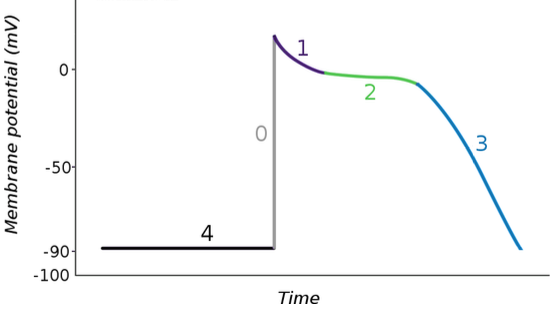
\includegraphics[width = 7cm]{./potential_cycle.png}
    \caption{Membrane potential in function of time (one cardiac cycle)}
    \label{potential_cycle}
    \end{center}
    \end{figure}
    
    \noindent The cell is initially at rest ($-90mV$, step 4). At a certain point, its potential increases rapidly ($\approx2ms$) and reaches the value of $+20mV$: the cell is activated. Later, a plateau near $0mV$ is observed and then a slow repolarization to the initial potential; cf. Fig. (\ref{potential_cycle}). \\
    From a microscopical point of view, we could study the dynamics acting in each single cell (as a consequence of the passage of chemical ions through specific channels, e.g. $Ca2+,Na+,K+$). From a macroscopical point of view, instead, one can describe it as a continuous electrical diffusion over the entire cardiac surface. Even if this consists in a very rapid phenomenon, the study of such propagation could be very interesting in order, for instance, to detect diseases in sick patients.
    
    \subsection{Mathematical models}
    Starting from the circuit in Figure (\ref{electrical_circuit}), applying general electromagnetism laws, the Bidomain model has been formulated (see \parencite{acta} for more details and/or \parencite{colli_franzone} for the complete derivation).
    
    \begin{figure}[h]
    	\begin{center}
    		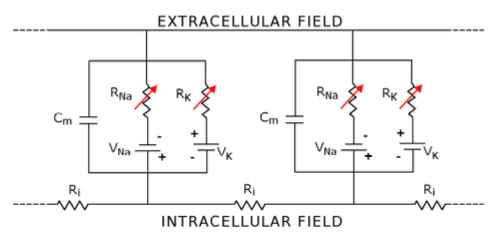
\includegraphics[width = 7cm]{./electrical_circuit.png}
    		\caption{Simplified circuit to model the intracellular and extracellular potential dynamics}
    		\label{electrical_circuit}
    	\end{center}
    \end{figure}
    
    \noindent The general formulation is the following: \vspace{3mm}
    \begin{problem}[Bidomain model]
    Find $\phi_i$ and $\phi_e$ such that:
	\begin{equation*}
	\begin{cases}
	\chi_m C_m\pdv{V_m}{t} - \nabla \cdot (\Sigma_i \nabla \phi_i) + \chi_m I_{ion} = I_i^{ext},    & \text{in } \Omega_{mus} \cross (0,T],
	\\
	\vspace{2mm}
	-\chi_m C_m\pdv{V_m}{t} - \nabla \cdot (\Sigma_e \nabla \phi_e) - \chi_m I_{ion} = -I_e^{ext},    & \text{in } \Omega_{mus} \cross (0,T].
	\end{cases}
	\end{equation*}
	\end{problem}
	\vspace{3mm}
	
	where:
	\begin{itemize}[label=\textendash]
		\item $\phi_i, \phi_e$ are the \emph{Intracellular and Extracelllular Potentials} (unknowns),
		\item $V_m = \phi_i-\phi_e$ is the \emph{Trans-membrane Potential},
		\item $\chi_m,C_m$ are known positive constants,
		\item $\Sigma_i, \Sigma_e$ are known positive definite tensors,
		\item $I_i^{ext},I_e^{ext}$ are applied currents,
		\item $I_{ion}$ is the \emph{Ionic Current},
		\item $\Omega_{mus}$ is the cardiac domain (myocardium + endocardium + epicardium).
	\end{itemize}
    
    \vspace{4mm}
    \noindent Actually, this system is not complete since it misses boundary and initial conditions and a suitable model for $I_{ion}$. Initial conditions and Neumann boundary conditions for $\phi_i$ and $\phi_e$ are then imposed. For the definition of $I_{ion}$, instead, a \emph{reduced ionic model} is chosen, in particular the \emph{FitzHugh-Nagumo model}. Summing up:\newpage
        \begin{problem}\label{def1}[Bidomain + FitzHugh-Nagumo model with Neumann boundary conditions]
      	Find $\phi_i$ and $\phi_e$ such that:
    	\begin{equation*}
    	\begin{cases}
    	\chi_m C_m\pdv{V_m}{t} - \nabla \cdot (\Sigma_i \nabla \phi_i) + \chi_m I_{ion}(V_m,w) = I_i^{ext},    & \text{in } \Omega_{mus} \cross (0,T],
    	\\
    	-\chi_m C_m\pdv{V_m}{t} - \nabla \cdot (\Sigma_e \nabla \phi_e) - \chi_m I_{ion}(V_m,w) = -I_e^{ext},    & \text{in } \Omega_{mus} \cross (0,T],
    	\\
    	I_{ion}(V_m,w)=kV_m(V_m-a)(V_m-1)+w, & \text{in } \Omega_{mus} \cross (0,T],
    	\\
    	\pdv{w}{t} = \epsilon(V_m-\gamma w),  & \text{in } \Omega_{mus} \cross (0,T],
    	\\
    	\Sigma_i\nabla \phi_i \cdot n = b_i,   & \text{on } \partial \Omega_{mus} \cross (0,T],
    	\\
    	\Sigma_e\nabla \phi_e \cdot n = b_e,   & \text{on } \partial \Omega_{mus} \cross (0,T],
    	\\
    	\text{Initial conditions for } \phi_i,\phi_e, w, & \text{in } \Omega_{mus}\cross\{t=0\}.
    	\end{cases}
    	\end{equation*}
    	\end{problem}
    \vspace{3mm}
    where:
    \begin{itemize}[label=\textendash]
    	\item $w$ is the \emph{gating variable} (unknown),
    	\item $k,a,\epsilon,\gamma$ are known constants,
    	\item $b_i,b_e$ are the boundary conditions data,
    	\item $n$ is the outward normal vector.
    \end{itemize}

    \vspace{4mm}
    \noindent From now on, the system of equations given by Problem (\ref{def1}) will be the reference analytical problem for the development of the forthcoming numerical schemes.\\
    To conclude, there exist other famous and useful models, such as the \emph{Monodomain model}, but this is just a simplification of the Bidomain as in this case it is assumed that $\phi_i$ and $\phi_e$ are proportional. However, thanks to its simplicity, we often tested the code starting from the Monodomain implementation of the project \cite{andreotti} instead of analyzing directly the Bidomain model reported.

    \subsection{State of the art}\label{past}
    As we have already introduced, our project initially aimed to continue and improve the work of a previous project \cite{marta}. \\
    Results obtained using unitary parameters, namely $\chi_m =\Sigma_i= \Sigma_e= C_m= k = \epsilon= \gamma= a=1$, were actually quite satisfactory. On the other hand, the choice of more realistic/experimental values for the parameters (that are often very big or very small) caused bad consequences to the accuracy of the schemes or even to their stability. In particular, we observed that the choice of $C_m \approx 10^{-2}$ highly compromised the stability of the numerical schemes (fact that was already noticed in \cite{andreotti}).
    This issue heavily limits the use of the \textsc{Matlab} code for research and/or experimental simulations as it guarantees convergence to the right solution only in few and non-realistic problems.  \\

   
\newpage

    \section{Semi-discrete Discontinuous Galerkin formulation}
    \subsection{Discontinuous Galerkin discrete formulation}
    Starting from the strong form given by the Problem (\ref{def1}), the next step is the achievement of a suitable Discontinuous Galerkin semi-discrete formulation. Full descriptions and justifications of all the terms are present in \cite{marta} . \\
    Let us introduce a triangulation $\tau_h$ over $\Omega$, where $\mathcal{F} _h=\mathcal{F} _h^I \cup \mathcal{F} _h^B$ on the set of the faces of the partition, which includes the internal ($\mathcal{F} _h^I$) and boundary ($\mathcal{F} _h^B$) faces. Let the DG space be defined as $V_h^p = \{v_h \in L^2(\Omega) : v_h|_\mathcal{K} \in \mathbb{P}^{p}(\mathcal{K})  \quad \forall \mathcal{K} \in \tau_h \}$, where $p$ is the degree of the piecewise continuous polynomial, i.e. $k \geq 1$. Moreover, we define $N_h=dim(V_h^p)<\infty$. \vspace{4mm}
    \begin{problem}[DG weak formulation]
    For any $t\in[0,T]$ find $\bm{\Phi_h}(t)=[\phi_i^h(t),\phi_e^h(t)]^T \in [V_h^p]^2$  and  $w_h(t) \in V_h^p$ such that:
    \begin{equation*}
    \begin{cases}
    \begin{gathered}
    \sum_{\mathcal{K} \in \tau_h} \int_{\mathcal{K}}{ \chi_m C_m \pdv{V_m^h}{t} V_h d\omega}+a_i(\phi_i^h,v_h)+\sum_{\mathcal{K} \in \tau_h} \int_{\mathcal{K}}{ \chi_m k (V_m^h-1)(V_m^h-a) V_m^h v_h d\omega}+\\
    +\sum_{\mathcal{K} \in \tau_h} \int_{\mathcal{K}}{ \chi_m w_h v_h d\omega}=(I_i^{ext},v_h), \qquad \forall v_h \in V_h^p,\\
    \vspace{2mm}
    \end{gathered}\\
    \begin{gathered}
    -\sum_{\mathcal{K} \in \tau_h} \int_{\mathcal{K}}{ \chi_m C_m \pdv{V_m^h}{t} V_h d\omega}+a_e(\phi_e^h,v_h)-\sum_{\mathcal{K} \in \tau_h} \int_{\mathcal{K}}{ \chi_m k (V_m^h-1)(V_m^h-a) V_m^h v_h d\omega}+\\
    -\sum_{\mathcal{K} \in \tau_h} \int_{\mathcal{K}}{ \chi_m w_h v_h d\omega}=(-I_e^{ext},v_h), \qquad \forall v_h \in V_h^p,\\
       \vspace{2mm}
    \end{gathered}\\
    \sum_{\mathcal{K} \in \tau_h} \int_{\mathcal{K}}{\pdv{w_h}{t}v_h d\omega}=\sum_{\mathcal{K} \in \tau_h} \int_{\mathcal{K}}{\epsilon (V_m^h-\gamma w_h) v_h d\omega}, \qquad \forall v_h \in V_h^p,\\
    \end{cases}
    \end{equation*}
    \vspace{5mm}
    where:
    \vspace{3mm}
    \begin{equation}\label{forgamma}
    \begin{aligned}
    \bullet& \quad a_l(\phi_l^h,v_h)=\sum_{\mathcal{K} \in \tau_h} \int_{\mathcal{K}}{(\Sigma_l \nabla_h \phi_k^h) \cdot \nabla_h v_h d\omega}-\sum_{F \in \mathcal{F}_h^I} \int_F { \{\{\Sigma_l \nabla_h \phi_l^h \}\} \cdot [[v_h]] d\sigma}+\\
    &-\delta \sum_{F \in \mathcal{F}_h^I} \int_F{ \{\{\Sigma_l \nabla_h v_h\}\} \cdot [[\phi_l^h]]d\sigma}+\sum_{F \in \mathcal{F}_h^I}\int_F {\Gamma [[\phi_l^h]] \cdot [[v_h]] d\sigma} \qquad l=i,e,\\
    \newline
    \bullet& \quad (I_i^{ext},v_h)=\sum_{\mathcal{K} \in \tau_h} \int_{\mathcal{K}} {I_i^{ext} v_h d\omega}+\int_{\partial \Omega}{b_i v_h d\sigma},\\
    \newline
    \bullet& \quad (-I_e^{ext},v_h)=-\sum_{\mathcal{K} \in \tau_h} \int_{\mathcal{K}} {I_e^{ext} v_h d\omega}+\int_{\partial \Omega}{b_e v_h d\sigma}.
    \end{aligned}
    \end{equation}
    
    \noindent Moreover, according to the choice of the coefficient $\delta$, we can define:
    \begin{itemize}
    \item $\delta=1$: Symmetric Interior Penalty method (SIP)
    \item $\delta=0$: Incomplete Interior Penalty method (IIP)
    \item $\delta=-1$: Non Symmetric Interior Penalty method (NIP) 
    \end{itemize}
     \vspace{2mm}
    \noindent In (\ref{forgamma}) $\Gamma$ is the so called stability parameter, which is defined edge-wise as:\\ $\Gamma := \alpha \frac{k^2}{h}$, where $ \alpha \in \mathbb{R}$ has to be chosen high enough for the SIP and IIP formulations.
    \end{problem}

    \subsection{Algebraic formulation}
    Taking $\{\varphi_j\}_{j=1}^{N_h}$ a basis of $V_h^p$, so that we can write
    \begin{equation*}
    \begin{gathered}
    \bm{\Phi_h}(t) = \begin{bmatrix} \phi_i^h(t) \\ \phi_e^h(t) \end{bmatrix} = \begin {bmatrix}\sum_{j=1}^{N_h} \phi_{i,j}(t)\varphi_j \\ \sum_{j=1}^{N_h} \phi_{e,j}(t)\varphi_j \end{bmatrix},\\
    w_h(t) = \sum_{j=1}^{N_h}w_j(t)\varphi_j,\\
    V_m^h(t)=\sum_{j=1}^{N_h} V_{m,j}(t) \phi_j=\sum_{j=1}^{N_h}(\phi_{i,j}(t)-\phi_{e,j}(t))\varphi_j.
 \end{gathered}
 \end{equation*}
 Where $\phi_{i,j}$, $\phi_{e,j}$ and $w_j \in \mathbb{R}$ are the unkonwn expansion coefficients $\forall$ i,j=1,...,$N_h$.
 Then, we introduce the matrices:
 \begin{equation*}
\begin{rcases}
(V_l)_{ij} &= \int_{\Omega}\nabla\varphi_j \cdot \Sigma_l \nabla \varphi_i,
\\ (I_l^T)_{ij} &= \sum_{F \in \mathcal{F}_h^I} \int_{F} \{\{\Sigma_l \nabla\varphi_j\}\} \cdot [[\varphi_i]],
\\ (I_l)_{i,j} &= \sum_{F \in \mathcal{F}_h^I} \int_{F} [[\varphi_j]] \cdot \{\{\Sigma_l \nabla \varphi_i\}\},
\\(S_l)_{i,j} &= \sum_{F \in \mathcal{F}_h^I} \int_{F} \Gamma_l[[\varphi_j]] \cdot [[\varphi_i]],
\end{rcases}
\begin{gathered}
\quad A_l = (V_l -I_l^T - \theta I_l + S_l)\\
l=i,e, \\
\end{gathered}
\end{equation*}
\begin{equation*}
\Gamma_l\vert_F = (n_F^T \, \Sigma_l \, n_F) \,\Gamma, \quad \text{with } n_F \text{ outward normal vector of F},
\end{equation*}
We also define:
\begin{equation*}
A_i \in \mathbb{R}^{N_h \times N_h} \qquad{\text{Intra-cellular stiffness matrix}},
\end{equation*}
\begin{equation*}
A_e \in \mathbb{R}^{N_h \times N_h} \qquad{\text{Extra-cellular stiffness matrix}},
\end{equation*}
\begin{equation*}
M_{ij} = \sum_{\mathcal{K} \in \tau_h}\int_{\mathcal{K}}\varphi_j\varphi_i \qquad{\text{Mass matrix}},
\end{equation*}
\begin{equation*}
C(u_h)_{ij} =  \sum_{\mathcal{K} \in \tau_h} \int_{\mathcal{K}} \chi_m k(u_h-1)(u_h-a)\varphi_j\varphi_i \qquad{\text{Non-linear matrix}},
\end{equation*}
\begin{equation*}
\bm{F_l}=\begin{bmatrix} F_{i,l} \\ F_{e,l} \end{bmatrix}=\begin{bmatrix} \int_{\Omega} I_i^{ext}\varphi_l - \sum_{F \in \mathcal{F}_h^B} \int_F b_i\varphi_l \\ - \int_{\Omega} I_e^{ext}\varphi_l - \sum_{F \in \mathcal{F}_h^B} \int_F b_e\varphi_l \end{bmatrix}.
\end{equation*}
\vspace{3mm} \\
Therefore, our semi-discrete algebraic formulation is as follows: \vspace{3mm}
\begin{problem}[DG algebraic formulation]\label{algebraic}
Find $\bm{\Phi_h}(t)=[\phi_i^h(t),\phi_e^h(t)]^T \in [V_h^p]^2$ and $w_h(t) \in V_h^p$ for any $t \in (0;T]$ such that:
\begin{equation*}
\begin{cases}
\chi_m Cm M \dot{V_m^h}+A_i \phi_i^h+C(V_m^h) V_m^h+\chi_m M w_h=F_i^h, \vspace{2mm} \\ 
-\chi_m Cm M \dot{V_m^h}+A_e \phi_e^h-C(V_m^h) V_m^h-\chi_m M w_h=F_e^h, \vspace{2mm} \\ 
M \dot{w}_h(t)=\epsilon M (V_m^h(t)-\gamma w_h(t)),
\end{cases}
\end{equation*}
\end{problem}
 \vspace{5mm}
 \noindent Supplement with suitable initial conditions.\\
 \noindent An alternative and more compact version is given by: \vspace{3mm}
 \begin{problem}[DG algebraic formulation - 2] \label{block_matrix}
 Find $\bm{\Phi_h}(t)=[\phi_i^h(t),\phi_e^h(t)]^T \in [V_h^p]^2$ and $w_h(t) \in V_h^p$ for any $t \in (0;T]$ such that:
 \begin{equation*}
 \begin{cases}
 \begin{gathered}
 \chi_mC_m \begin{bmatrix}M &-M \\ -M & M \end{bmatrix}
	\begin{bmatrix}\dot{\phi}_i^h(t) \\ \dot{\phi}_e^h(t) \end{bmatrix}
	 + \begin{bmatrix}A_i & 0 \\ 0 & A_e \end{bmatrix}
	 \begin{bmatrix}\phi_i^h(t) \\ \phi_e^h(t) \end{bmatrix} +
	   \begin{bmatrix}C(V_m^h) & -C(V_m^h) \\ -C(V_m^h) & C(V_m^h) \end{bmatrix} 
	   \begin{bmatrix} \phi_i^h(t) \\ \phi_e^h(t)  \end{bmatrix}+\\
	   +\chi_m \begin{bmatrix}M & 0 \\ 0 & -M \end{bmatrix} 
	   	\begin{bmatrix}w_h(t) \\ w_h(t) \end{bmatrix} = 
	   	\begin{bmatrix} F_i^h \\ F_e^h\end{bmatrix},
	   	\end{gathered}\\
	   	\vspace{3mm} 
	   \dot{w}_h(t)=\epsilon (V_m^h(t)-\gamma w_h(t)).
\end{cases}
\end{equation*}
\end{problem}
\newpage
\section{High-order Dubiner basis functions}
    \subsection{Analytical aspects}\label{analytical_aspects}
    So far, we have described a general semi-discrete discontinuous formulation without examining which basis to use to generate the $V_h^p$ space. Usually, the common choice consists in the classical hat functions from FEMs. It is also one of the simplest choices, for this reason our provided code was initially implemented with this basis. However, the very novelty of this study is the adoption of a new kind of basis, completely different from the previous and commonly known as "\emph{Dubiner basis}"\cite{dubiner}, which is well suited to high-order approximations. \\
    How we will see soon, the peculiarity of this family of functions is that it consists of orthogonal polynomials defined on the reference triangle
    \begin{equation*}
    \hat{K}=\{ (\xi, \eta) : \xi, \eta \ge 0,	\xi+\eta \le 1 \},
    \end{equation*}
    and not on the reference square
    \begin{equation*}
    \quad \quad \hat{Q}=\{ (a, b) : -1 \le a \le 1, -1 \le b \le 1 \}.
    \end{equation*}
    Formally, if we consider the transformation from $\hat{Q}$ to $\hat{K}$ is given by:
    \begin{equation}\label{transformation_formula}
    \xi=\frac{(1+a)(1-b)}{4},  \eta=\frac{(1+b)}{2},
    \end{equation}
    
    \begin{figure}[h]
    \begin{center}
    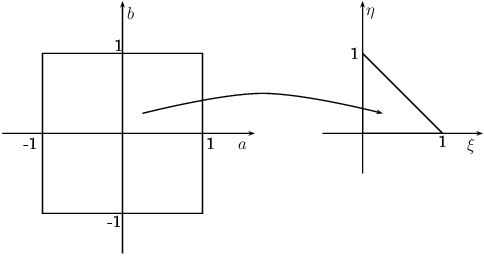
\includegraphics[width = 7cm]{./transformation.png}
    	\caption{Transformation between the reference square ($\hat{Q}$) to the reference triangle ($\hat{K}$)}
    	\label{transformation}
    \end{center}
    \end{figure}
    
    \noindent the Dubiner basis is the transformation of a suitable basis initially defined on the reference square. This initial basis is simply obtained with a two dimensional modified tensor product of the Jacobi polynomials on the interval $(-1,1)$, as described in the following definition. \\

    \begin{definition}[Jacobi polynomials]\label{jacobi}
    The Jacobi polynomials of coefficients $\alpha,\beta \in \mathbb{R}$ evaluated in $z\in (-1,1)$ are:
    \begin{itemize}[label=\textendash]
    \item $n=0$
    \begin{equation*}
    J_0^{\alpha,\beta}(z)=1,
    \end{equation*}
    \item $n=1$
    \begin{equation*}
    J_1^{\alpha,\beta}(z)=\frac{1}{2}(\alpha-\beta+(\alpha+\beta+2)\cdot z),
    \end{equation*}
    \item $n\ge2$
    \newline
    \begin{equation*}
    \begin{gathered}
    \begin{aligned}
    J_n^{\alpha,\beta}(z)=\sum_{k=2}^{n} \Big[&\frac{(2k+\alpha+\beta-1)(\alpha^{2}-\beta^{2})}{2k(k+\alpha+\beta)(2k+\alpha+\beta-2)}+ \\ &\frac{(2k+\alpha+\beta-2)(2k+\alpha+\beta-1)(2k+\alpha \beta)}{2k(k+\alpha+\beta)(2k+\alpha+\beta-2)} J_{k-1}^{\alpha,\beta}(z) +
    \\-&\frac{2(k+\alpha-1)(k+\beta-1)(2k+\alpha+\beta)}{2k(k+\alpha+\beta)(2k+\alpha+\beta-2)} J_{k-2}^{\alpha,\beta}(z) \Big].
    \end{aligned}
    \end{gathered}
    \end{equation*}
    \end{itemize}
    \end{definition}
    \vspace{5mm}
    \noindent The main property of these polynomials is the following:
    \begin{prop}\label{prop1}
    $\{J_i^{\alpha,\beta}, \, i=0,1,2 \dots\}$ is orthogonal with respect to the Jacobi weight $w(x)=(1-x)^\alpha(1+x)^\beta$, i.e.:
    \begin{equation*}
    \int_{-1}^{1}{(1-x)^\alpha(1+x)^\beta J_m^{\alpha,\beta}(x) J_q^{\alpha,\beta}(x)dx}=\frac{2}{2m+1} \delta_{mq} \qquad \forall i,j,m,q \geq 0.
    \end{equation*}
    \end{prop}
    
    \noindent We can now define explicitly the Dubiner basis.
    \begin{definition}[Dubiner basis] \label{dubiner}
    The Dubiner basis that generates the space $\mathbb{P}^p(\hat{K})$ of polynomials of degree $p$ over the reference triangle is the set of functions:
    \begin{equation*}
    \begin{split}
    \\
    & \quad \quad\quad  \quad \phi_{ij}: \hat{K} \rightarrow \mathbb{R}, \\ \\
    \phi_{ij}(\xi,\eta) :&= c_{ij}(1-b)^j J_i^{0,0}(a) J_j^{2i+1,0}(b)=
    \\&=c_{ij} 2^j (1-\eta)^j J_i^{0,0}(\frac{2\xi}{1-\eta}-1) J_j^{2i+1,0} (2\eta-1),
    \end{split}
    \end{equation*}
    \vspace{3mm} \\
    for $i,j=0,\dots,p$ and $i+j \le p$, where
    \begin{equation*}
    c_{ij} := \sqrt{\frac{2(2i+1)(i+j+1)}{4^i}}
    \end{equation*}
    and $J_i^{\alpha,\beta}(\cdot)$ is the i-th Jacobi polynomial defined in Definition (\ref{jacobi}).
    \end{definition}
    
    \vspace{5mm}
    \noindent As we have anticipated the following result holds, cf.  \cite{sherwin}.
    \begin{prop}\label{l2_ortho}
    The Dubiner basis is orthonormal in $L^2(\hat{K})$ $\forall p \geq 0$:
    \begin{equation*}
    \int_{\hat{K}}{\phi_{ij}(\xi,\eta)\phi_{mq}(\xi,\eta) d\xi d\eta}=\delta_{im}\delta_{jq} \qquad \forall i,j,m,q \geq 0.
    \end{equation*}
    \end{prop}
    \vspace{4mm}
    \noindent Notice that, thanks to the Proposition (\ref{l2_ortho}), the mass matrix of the DG space turns out to be diagonal. See Fig. (\ref{mass}) as an example.
    
    \begin{figure}[ht]
    \begin{center}
    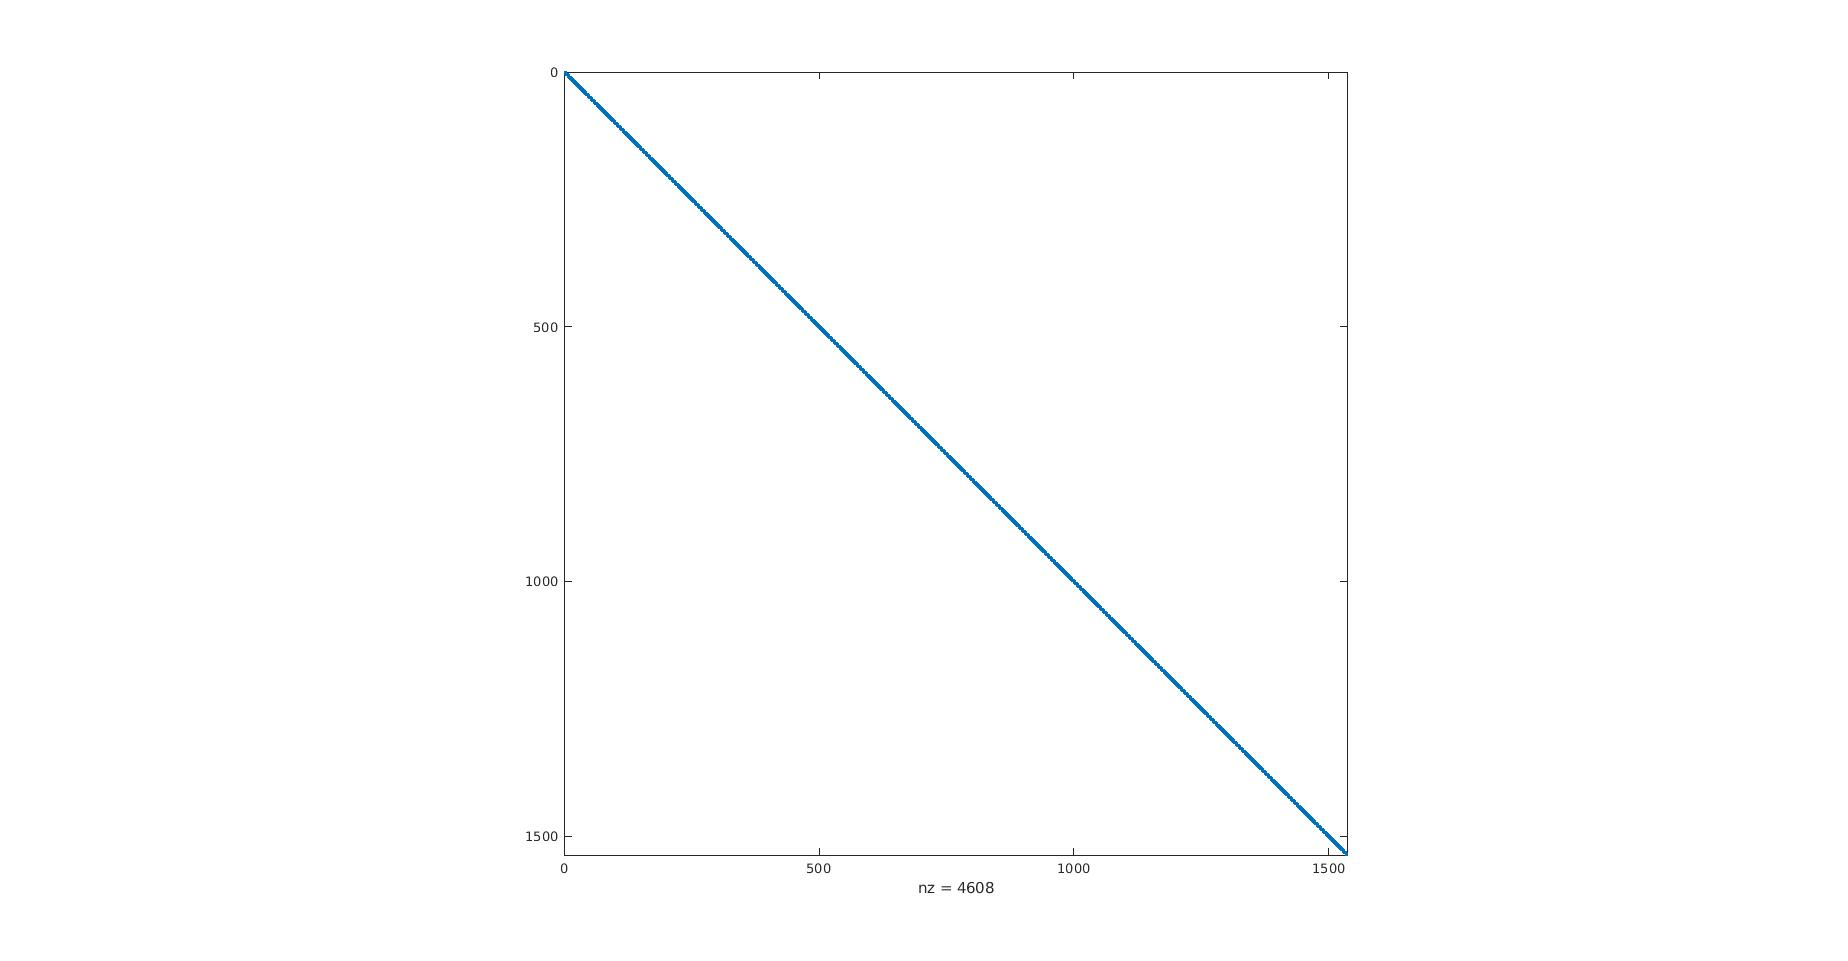
\includegraphics[width = 10cm]{./mass_dubiner.jpg}
    	\caption{Non-zero elements in the mass matrix when adopting Dubiner basis}
    	\label{mass}
    \end{center}
    \end{figure}

    \noindent It is noteworthy to point out that transformation (\ref{transformation_formula}) is bijective, it can be inverted but it needs some care. The natural inverse would be:
    
    \begin{equation*}
    a = \frac{2\xi}{1-\eta}-1 \quad \quad b = 2\eta-1,
    \end{equation*}
    \vspace{2mm} \\
    \noindent that has already been used for the Definition (\ref{dubiner}). However, it is not defined for $\eta=1$, that means for the sole point $(0,1)$ of the reference triangle. To solve this issue, it is enough to prolongate the function with continuity to this special point. For the code implementation, it is suggested avoiding evaluations in the exact point, which can be avoided using quadrature formula of Gaussian type. \\
    
    \noindent In general, the orthogonality property implies some good numerical properties, not only the diagonalization of the mass matrix. For instance, in \cite{antonietti} interesting bounds for the conditional number have been proved. For this reason, we opted for this choice aiming to improve the previous results, at least from the space discretization side. \\
    
    \noindent On the other hand, there are also some difficulties arising when one chooses to abandon the familiar FEM basis. First of all, the coefficients of a discretized function has only \emph{modal} meaning and they no more represent the \emph{nodal} values of the function itself. This fact needs some extra work when one needs to switch from the continuous functions to the discretized functions and viceversa, as it will be shown in the Section (\ref{subsection_implementation}). Secondly, one can notice that these functions are not "boundary conditions friendly". What we mean is that, if compared to FEM basis, they have no particular properties on the boundary to let easily impose homogeneous boundary conditions. Thus, they should be again transformed, this time in a \emph{boundary adapted} form. We address to \cite{napde} for a short description of this procedure. Fortunately, we do not need to set this transformation as in the discontinuous formulation Dirichlet boundary conditions are imposed only weakly. It means that the boundary conditions' choice does not imply the choice of the vectorial space as in continuous Galerkin methods. The discretized space is always the same, only some terms in the weak formulation have in case of need to be changed. For this reason, the match of Discontinuous Galerkin and Dubiner basis results to be particularly successful. \\
    
    \noindent To conclude, we refer to \cite{sherwin} for the transformation and the definition of the Dubiner basis with tetrahedra, i.e. in dimension $n=3$.
    
    \subsection{Implementation}\label{subsection_implementation}
    Our \textsc{Matlab} code allows the user to select which basis to adopt (FEM or Dubiner) and the order of polynomials until p=3. We chose to call $D_1,D_2,D_3$ these 3 families of basis functions, thanks to the similarity to the $P_1,P_2,P_3$, finite element basis functions.\\
    As explained in Section (\ref{past}), our starting point was the code implemented by the previous projects, namely the resolution of the Bidomain Model throught FEM basis ($P_1,P_2,P_3$). As follows, our first goal was the implementation of methods to evaluate the Dubiner basis functions ($D_1,D_2,D_3$) and their gradients in the quadrature points. We omit the full code as it is not particular interesting: it barely follows the definitions of Section (\ref{analytical_aspects}) with the addition of some technicalities. These scripts are: \texttt{eval\_jacobi\_polynomial.m}, \texttt{basis\_legendre\_dubiner.m}, \texttt{evalshape\_tria\_dubiner.m}.\\
    
    \noindent Moreover, some conditional statements and some extra methods (as \texttt{matrix2D\_dubiner.m}) were added to let the user easily switch from one basis to another (simply and once via \texttt{dati.m}). \\
    
    \noindent More interesting are instead the scripts \texttt{dubiner\_to\_fem.m} and \texttt{fem\_to\_dubiner.m}, used to convert the Dubiner modal coefficients of the vector solution to the nodal values of the approximated function and viceversa. For this reason, they deserve some further explanations.
\subsection{Switch from the modal expansion coefficients to the Lagrangian ones}
One of the many advantages of the FEM basis is that there exists a bijection between the basis functions and some particular spacial points in such a way that the evaluation of a basis function in one of these points is equal to 1 only if that point is the one associated to the function and 0 otherwise, i.e.:
	\begin{equation} \label{ref1}
	\psi_i(x_j)=\delta_{ij}.
	\end{equation}
	Obviously, this property does not hold when we work with the Dubiner basis. Indeed, these functions are not associated to any mesh point. This implies that the Dubiner coefficients of a function $u\in V_h^p$ are not the evaluation at suitable points of the discretized function itself. They have a completely different meaning, they are now \emph{modal} values instead of being \emph{nodal}.
	For this reason we introduced two new functions that transform the coefficients of the solution w.r.t. the FEM basis to the coefficients w.r.t. the Dubiner basis and viceversa.\vspace{5mm}
	
	\noindent Consider an element $\mathcal{K}\in \tau_h$ and $\{\psi_{i}\}_{i=1}^{p}$,$\{\phi_{j}\}_{j=1}^{q}$ as, respectively, the set of FEM functions and the set of Dubiner functions with support in $\mathcal{K}$. In addition, consider as $\{\hat{u}_i\}_{i=1}^p$,$\{\tilde{u}_j\}_{j=1}^q$ as, respectively, the FEM and Dubiner coefficients of the solution.
	
	\subsubsection{From Dubiner basis to FEM basis}
	\noindent Let us start from the transformation to the FEM coefficients. We now exploit the Property (\ref{ref1}), i.e. the coefficient $\hat{u}_i$ is nothing else but the evaluation of $u_h$ on the i-th mesh point, then: 
	\begin{equation} \label{ref3}
	\hat{u}_i = \sum_{j=1}^q \tilde{u}_j\phi_j(x_i),
	\end{equation}
	where $x_i$ is the point associated to the $\psi_i$ basis function. \\
	This formula has been implemented in the lines from \texttt{dubiner\_to\_fem.m} script (Section (\ref{dub_to_fem})).

	\subsubsection{From FEM basis to Dubiner basis}
	\noindent Instead, to compute the coefficients conversely, we need to exploit the fact that the Dubiner basis is $L^2$-orthonormal (Proposition \ref{l2_ortho}). We then need to compute a $L^2$ scalar product between the FEM discretized function and each Dubiner basis function. That is:
	\begin{equation}\label{ref4}
	\tilde{u}_j = \int_\mathcal{K} u_h(x) \phi_j(x) \,dx = \int_{\mathcal{K}} \sum_{i=1}^p \hat{u}_i\psi_i(x) \phi_j(x) \,dx = \sum_{i=1}^p \Big(\int_{\mathcal{K}}\psi_i(x)\phi_j(x)\,dx \Big) \hat{u}_i, \qquad j=1,...
	\end{equation}
	\vspace{2mm} \\
	\noindent This slightly more difficult formula has been reproduced in \texttt{fem\_to\_dubiner.m} (Section (\ref{fem_to_dub})) using \emph{Gauss-Legendre} quadrature formulas.
	\subsubsection{Final remarks}\label{dub}
	\noindent If the Dubiner functions are chosen as Galerkin basis, both the transformations are needed for the code implementation. Formula (\ref{ref3}) is needed to plot and compute errors after the solution of the system. Formula (\ref{ref4}) is instead needed to convert the FEM initial data $u_0$ into a vector of Dubiner coefficients before the resolution of the system.\\
	
	\noindent In order to be rigorous, but also for the sake of simplicity, these transformations are implemented only from $P_n$ to $D_n$, $n=1,2,3$ and viceversa, where $P_n$ means the FEM basis of n-th polynomial degree, meanwhile $D_n$ is for the Dubiner basis of n-th polynomial degree. With this choice, the two bases generate the same space $V_h^p$ and then the transformation infers only on the coefficients and not on the function's properties. Otherwise, decreasing $n$ would mean to lose significant information, while increasing $n$ does not substantially improve the quality of the solution as it initially belonged to a lower order space. Moreover, choosing the same degree for P and D implies several semplifications, for instance the same number of local nodes ($nln$). For this reason, both $p$ and $q$ are actually replaced with $nln$ in the code.
	

\newpage 
\section{Temporal discretization}\label{temporal_discretization}
So far, we have just studied the space discretization while a temporal discretization is still needed to totally discretize the Bidomain time-dependent problem. Thus, we divide the interval (0,T] into N subintervals $(t^n,t^n+1]$ of length $\Delta t$ such that $t^n=n \Delta t \quad \forall n=0,\cdots,N-1$, we then assume our fully discretized solution as $V_m^n\approx V_m^h(t^n)$. \\
We have developed, implemented and tested 3 different temporal strategies that we will refer to as: \emph{semi-implicit}, \emph{Godunov operator-splitting} and \emph{quasi-implicit operator-splitting}. 
\subsection{The semi-implicit method}
One of the most famous and used temporal scheme for a non-linear problem such as the Bidomain is certainly the \emph{Semi-Implicit} scheme \cite{acta}. The basic idea is to treat most of the terms implicitly while treating the non-linear term semi-implicitly. Since the non-linear term is cubic, the best choice is to treat only one of these $V_m$ terms implicitly, i.e.:
\begin{equation*}
I_{ion}^{n+1}=k(V_m^n-a)(V_m^n-1)V_m^{n+1}+w^{n+1},
\end{equation*}
at each time-step $n+1$. 
Moreover, the gating variable ODE is treated implicitly with the exception of the term $V_m$:
\begin{equation*}
M \frac{w^{n+1}-w^n}{\Delta t}=\epsilon M (V_m^n-\gamma w^{n+1}).
\end{equation*}
\vspace{5mm} \\
Therefore, we can transform the semi-discrete Problem (\ref{block_matrix}) into:
\begin{equation*}
\begin{cases}
 \begin{gathered}
 \chi_mC_m \begin{bmatrix}M &-M \\ -M & M \end{bmatrix}
	\begin{bmatrix}\frac{\phi_i^{n+1}-\phi_i^{n}}{\Delta t} \\ \frac{\phi_e^{n+1}-\phi_e^{n}}{\Delta t}  \end{bmatrix}
	 + \begin{bmatrix}A_i & 0 \\ 0 & A_e \end{bmatrix}
	 \begin{bmatrix}\phi_i^{n+1} \\ \phi_e^{n+1} \end{bmatrix} +\\
	   \begin{bmatrix}C(V_m^h) & -C(V_m^h) \\ -C(V_m^h) & C(V_m^h) \end{bmatrix} 
	   \begin{bmatrix} \phi_i^{n+1} \\ \phi_e^{n+1}  \end{bmatrix} 
	   +\chi_m \begin{bmatrix}M & 0 \\ 0 & -M \end{bmatrix} 
	   	\begin{bmatrix}w^{n+1} \\ w^{n+1} \end{bmatrix} = 
	   	\begin{bmatrix} F_i^{n+1} \\ F_e^{n+1}\end{bmatrix},\vspace{2mm}\\
	   M \frac{w^{n+1}-w^n}{\Delta t}=\epsilon M (V_m^n-\gamma w^{n+1}).
\end{gathered}
\end{cases}
\end{equation*}\\
We remind that $V_m^n=\phi_i^n-\phi_e^n$. Separating known and unknown terms, we obtain: \vspace{3mm}
\begin{equation*}
\begin{cases}
\begin{gathered}
\left( \frac{\chi_m C_m}{\Delta t} \begin{bmatrix} M & -M \\ -M & M \end{bmatrix} + \begin{bmatrix} A_i & 0 \\ 0 & A_e \end{bmatrix} + 
\begin{bmatrix}
C(V_m^n) & -C(V_m^n) \\ -C(V_m^n) & C(V_m^n)
\end{bmatrix}\right)
\begin{bmatrix} \phi_i^{n+1} \\ \phi_e^{n+1} \end{bmatrix} = 
\\
\begin{bmatrix} F_i^{n+1} \\ F_e^{n+1} \end{bmatrix} 
- \chi_m \begin{bmatrix}M & 0 \\ 0 & -M \end{bmatrix}
\begin{bmatrix} w^{n+1} \\ w^{n+1} \end{bmatrix}
+ \frac{\chi_m C_m}{\Delta t} \begin{bmatrix}M & 0 \\ 0 & -M\end{bmatrix}
\begin{bmatrix} V_m^{n} \\ V_m^{n} \end{bmatrix}, \vspace{2mm}\\
(\frac{1}{\Delta t}+\epsilon \gamma)M w^{n+1}=\epsilon M V_m^n+\frac{M}{\Delta t} w^n.
\end{gathered}
\end{cases}
\end{equation*}

\vspace{5mm}
\noindent If we define:
\begin{itemize}
\item $B=\frac{\chi_m C_m}{\Delta t} \begin{bmatrix} M &-M \\-M & M \end{bmatrix}+\begin{bmatrix} A_i & 0 \\ 0 & A_e \end{bmatrix}$,
\item $C_{nl}(V_m^n)=\begin{bmatrix}C(V_m^h) & -C(V_m^h) \\ -C(V_m^h) & C(V_m^h) \end{bmatrix}$,
\item $r^{n+1}=\begin{bmatrix} F_i^{n+1} \\ F_e^{n+1}\end{bmatrix}-\chi_m \begin{bmatrix}M & 0 \\ 0 & -M \end{bmatrix} \begin{bmatrix}w^{n+1} \\ w^{n+1} \end{bmatrix}+\frac{\chi_m C_m}{\Delta t} \begin{bmatrix} M &-M \\-M & M \end{bmatrix} \begin{bmatrix} \phi_i^n \\ \phi_e^n \end{bmatrix}$,
\end{itemize} \vspace{5mm}
we get the system in its final form.  \\
\begin{problem}[Semi-implicit discretized system]
Find $\bm{\Phi^{n+1}}=[\phi_i^{n+1} \phi_e^{n+1}]^T$ and $w^{n+1}$ $\forall n=0,\cdots,N-1$ such that:
\begin{equation*}
\begin{cases}
(\frac{1}{\Delta t}+\epsilon \gamma)M w^{n+1}=\epsilon M V_m^n+\frac{M}{\Delta t} w^n, \vspace{2mm} \\
(B+C_{nl}(\bm{\Phi^n})) \bm{\Phi^{n+1}}=r^{n+1}.
\end{cases}
\end{equation*} 
\end{problem}

\noindent The implementation can be found at Section (\ref{SI}).

\subsection{The Godunov operator-splitting}
The main feature of a general operator-splitting method is the sub-division of the problem into two different problems to be solved sequentially. This is possible and justified when the original functional operator $L$ is splitted into 2 different operators such that $L(u)=L_1(u)+L_2(u)$.
Two operator-splitting methods have been implemented, the first is of \emph{Godunov} type and a detailed study together with its properties can be found in \cite{spiteri}. The formulation is: \\ \\
\begin{center}Find $\hat{V}_m^{n+1},\phi_i^{n+1},\phi_e^{n+1},w^{n+1}$ such that:\end{center}
\begin{equation*}
\begin{cases}
\chi_m C_m M\frac{\hat{V}_m^{n+1} - V_m^n}{\Delta t} + C(V_m^n)V_m^n +\chi_mMw^n = 0,\vspace{2mm}\\
\frac{w^{n+1}-w^n}{\Delta t} = \epsilon (V_m^n - \gamma w^n).
\end{cases}
\end{equation*}
\vspace{3mm}
\begin{equation*}
\begin{cases}
\chi_m C_m M\frac{V_m^{n+1} - \hat{V}_m^{n+1}}{\Delta t} + A_i\phi_i^{n+1} = F_i^{n+1}, \vspace{2mm}\\
-\chi_m C_m M\frac{V_m^{n+1} - \hat{V}_m^{n+1}}{\Delta t} + A_e\phi_e^{n+1} = F_e^{n+1}.
\end{cases}
\end{equation*}
\vspace{3mm}
\noindent Putting in a unique system:
\begin{equation}\label{Godunov}
\begin{cases}
\chi_m C_m M\frac{V_m^{n+1} - V_m^n}{\Delta t} + C(V_m^n)V_m^n +\chi_mMw^n + A_i \phi_i^{n+1}= F_i^{n+1}, \vspace{2mm}\\
\chi_m C_m M\frac{V_m^{n+1} - V_m^n}{\Delta t} + C(V_m^n)V_m^n +\chi_mMw^n - A_e \phi_e^{n+1}= -F_e^{n+1}, \vspace{2mm}\\
w^{n+1} = (1-\epsilon \gamma \Delta t) w^n + \epsilon \Delta t V_m^n.
\end{cases}
\end{equation} \vspace{3mm} \\
The equations in the system (\ref{Godunov}) can be rewritten as:
\begin{equation*}
\begin{cases}
\left( \frac{\chi_m C_m}{\Delta t} M + A_i \right ) \phi_i^{n+1} - \frac{\chi_m C_m}{\Delta t} M \phi_e^{n+1} = F_i^{n+1} - \chi_m M w^n + \left( \frac{\chi_m C_m}{\Delta t} M- C(V_m^n)\right) V_m^n,\vspace{2mm}\\
\frac{\chi_m C_m}{\Delta t} M  \phi_i^{n+1} - \left(\frac{\chi_m C_m}{\Delta t} M + A_e \right) \phi_e^{n+1} =  -F_e^{n+1} - \chi_m M w^n + \left( \frac{\chi_m C_m}{\Delta t} M- C(V_m^n)\right) V_m^n, \vspace{2mm}\\
w^{n+1} = (1-\epsilon \gamma \Delta t) w^n + \epsilon \Delta tV_m^n.
\end{cases}
\end{equation*}

\noindent Then, we obtain the final form:
\begin{problem}[Godunov operator-splitting discretized system] 
	Find $\bm{\Phi^{n+1}}=[\phi_i^{n+1} \phi_e^{n+1}]^T$ and $w^{n+1} \quad \forall n=0, \cdots, N-1$ such that: 
\begin{equation*}
\begin{cases}
\begin{gathered}
\left(
\frac{\chi_m C_m}{\Delta t} \begin{bmatrix}M & -M \\ M & -M\end{bmatrix}
+ \begin{bmatrix} A_i & 0 \\ 0 & -A_e \end{bmatrix}
\right) \begin{bmatrix} \bm{\phi_i^{n+1}} \\ \bm{\phi_e^{n+1}}  \end{bmatrix} =
\begin{bmatrix} F_i^{n+1} \\ -F_e^{n+1} \end{bmatrix} + \\ -
\chi_m\begin{bmatrix} M & 0 \\ 0 & M \end{bmatrix} \begin{bmatrix} w^n \\ w^n \end{bmatrix} +
\left(\frac{\chi_mC_m}{\Delta t}\begin{bmatrix} M & 0 \\ 0 & M \end{bmatrix}
- \begin{bmatrix} C(V_m^n) & 0 \\ 0 & C(V_m^n)\end{bmatrix} 
\right) \begin{bmatrix} V_m^n \\ V_m^n \end {bmatrix},
\end{gathered} \vspace{2mm}\\ \\
w^{n+1} = (1-\epsilon \gamma \Delta t) w^n + \epsilon \Delta tV_m^n.
\end{cases}
\end{equation*}
\end{problem}\vspace{4mm}
\noindent The implementation is written at Section (\ref{GO}).

\subsection{The quasi-implicit operator-splitting}
The aim of a quasi-implicit operator splitting is to treat implicitly all the terms except the cubic one. Even if it cannot be defined as a fully implicit method, we hope to achieve more stability if compared to the previous Godunov-kind scheme. This time, the formulation turns to be: \newline

\begin{center} Find $\tilde{V}_m^{n+1}, \phi_i^{n+1}, \phi_e^{n+1},w^{n+1}$ such that: \end{center}
\begin{equation*}
\begin{cases}
\chi_m C_m M \frac{\tilde{V}_m^{n+1}-V_m^n}{\Delta t} +  C(V_m^n) V_m^{n+1} + \chi_m M w^{n+1}= 0,\vspace{2mm}\\
\frac{w^{n+1} - w^n}{\Delta t} = \epsilon (V_m^{n+1}-\gamma w^{n+1}).
\end{cases}
\end{equation*}
\vspace{3mm}
\begin{equation*}
\begin{cases}
\chi_m C_m M \frac{V_m^{n+1}-\tilde{V}_m^{n+1}}{\Delta t} + A_i \phi_i^{n+1}= F_i^{n+1},\vspace{2mm}\\
- \chi_m C_m M \frac{V_m^{n+1}-\tilde{V}_m^{n+1}}{\Delta t} + A_e \phi_e^{n+1}= F_e^{n+1}.
\end{cases}
\end{equation*}
\vspace{3mm}
Putting into a unique system, we obtain:
\begin{equation}\label{Quasi}
\begin{cases}
\chi_m C_m M \frac{V_m^{n+1}-V_m^{n}}{\Delta t} + C(V_m^n) V_m^{n+1} + \chi_m M w^{n+1} + A_i \phi_i ^{n+1} = F_i^{n+1}, \vspace{2mm}\\
\chi_m C_m M \frac{V_m^{n+1}-V_m^{n}}{\Delta t} +  C(V_m^n) V_m^{n+1} + \chi_m M w^{n+1} - A_e \phi_e ^{n+1} =  -F_e^{n+1},\vspace{2mm} \\
\frac{w^{n+1}-w^{n}}{\Delta t} = \epsilon(V_m^{n+1}-\gamma w^{n+1}).
\end{cases}
\end{equation} 
\vspace{2mm} \\
If we define:
\begin{itemize}
\item $Q_n = \frac{\chi_m C_m}{\Delta t}M + C(V_m^n) + \frac{\epsilon\chi_m \Delta t}{1 + \epsilon \gamma \Delta t} M$,
\item $R_n = \frac{\chi_mC_m}{\Delta t}MV_m^n - \frac{\chi_m}{1+\epsilon\gamma\Delta t}M w^n$,
\end{itemize}
\vspace{4mm}
the equations in system (\ref{Quasi}) can be written as:
\begin{equation}
\begin{gathered}
\chi_m C_m M \frac{	\phi_i^{n+1}-\phi_e^{n+1}-V_m^{n}}{\Delta t} +  C(V_m^n) (\phi_i^{n+1}-\phi_e^{n+1}) + \\
 +\chi_m M \left(\frac{w^n + \epsilon \Delta t (\phi_i^{n+1}-\phi_e^{n+1})}{1+\epsilon \gamma \Delta t}   \right)
+ A_i \phi_i ^{n+1} = F_i^{n+1}, \\ \\
\Rightarrow \quad (Q_n + A_i) \phi_i^{n+1} - Q_n \phi_e^{n+1} =R_n +  F_i^{n+1},
\end{gathered}
\end{equation}
\vspace{3mm}
\begin{equation}
\begin{gathered}
\chi_m C_m M \frac{	\phi_i^{n+1}-\phi_e^{n+1}-V_m^{n}}{\Delta t} + \cdot C(V_m^n) (\phi_i^{n+1}-\phi_e^{n+1}) +\\ 
+ \chi_m M \left(\frac{w^n + \epsilon \Delta t (\phi_i^{n+1}-\phi_e^{n+1})}{1+\epsilon \gamma \Delta t}   \right)
- A_e \phi_e ^{n+1} = -F_e^{n+1}, \\ \\
\Rightarrow \quad Q_n \phi_i^{n+1} - (Q_n+A_e) \phi_e^{n+1} =R_n - F_e^{n+1},
\end{gathered}
\end{equation}
\vspace{3mm}
\begin{equation}
w^{n+1} = \frac{w^n + \epsilon \Delta t (\phi_i^{n+1}-\phi_e^{n+1})}{1+\epsilon \gamma \Delta t}.
\end{equation}
The final system becomes: \\
\begin{problem} [Quasi-implicit operator-splitting discretized system]
Find $\bm{\Phi^{n+1}}=[\phi_i^{n+1} \phi_e^{n+1}]^T$ and $w^{n+1} \quad \forall n=0, \cdots, N-1$ such that:
\begin{equation*}
\quad
\begin{cases}
\left(
\begin{bmatrix} Q_n & -Q_n \\ Q_n & -Q_n \end{bmatrix} + 
\begin{bmatrix} A_i & 0 \\ 0 & -A_e\end{bmatrix}
\right)
\begin{bmatrix}
\phi_i^{n+1} \\ \phi_e^{n+1}
\end{bmatrix}
= \begin{bmatrix} R_n \\ R_n \end{bmatrix} + \begin{bmatrix} F_i^{n+1} \\  -F_e^{n+1}\end{bmatrix},\\ \\
w^{n+1} = \frac{\displaystyle w^n + \epsilon \Delta t (\phi_i^{n+1}-\phi_e^{n+1})}{\displaystyle 1+\epsilon \gamma \Delta t}.
\end{cases}
\end{equation*}
\end{problem}
\vspace{4mm}
\noindent The implementation is shown at Section (\ref{OS}).
\newpage
\section{About uniqueness of the potentials}\label{unique}
\subsection{Analytical concepts}
\noindent Observing for a moment the Bidomain problem analytical formulation (Problem (\ref{def1})), we can immediately realize that the intracellular and the extracellular potentials appear only through their difference $V_m$ or their gradient. This means that there cannot be uniqueness for the two functions. Namely: \vspace{2mm}
\begin{equation}\label{phi_uniqueness}
\begin{gathered}
\phi_i,\phi_e \text{ classical solutions of Bidomain} \Rightarrow \phi_i+\varphi,\,\phi_e+\varphi \text{ are solutions as well } \\
 \forall \varphi: [0,T] \rightarrow \mathbb{R} \quad \text{ sufficiently regular}.
\end{gathered}
\end{equation}

\vspace{4mm}
\noindent However, this fact should not surprise nor confuse the reader. First of all, we remind again that in \cite{bourgault} and \cite{colli_franzone} there are proofs for the $V_m$ and $w$ uniqueness, then this is taken for granted. Secondly, this statement reflects the physical intuition of the problem: cellular dynamics is not involved by potentials exact values but instead from their difference, in addition a potential value is nonsense if a convention value to compare it with has not been set. The dependence on time can be interpreted as follows: if, at any time instant, we change the conventional potential value, the dynamics of the problem does not change. \\

\noindent Moreover, we can give this simple result to show that the solutions of the form of equation (\ref{phi_uniqueness}) are also the only admissible:\\
\begin{theo}
	For the Bidomain problem coupled with Fitzhugh-Nagumo model with Neumann boundary conditions (Problem (\ref{def1})), the classical solutions $\phi_i,\phi_e$ are unique up to a constant depending only on time. 
\end{theo}

\begin{proof}
	\vspace{2mm} We remind that existence and uniqueness for $V_m$ and $w$ have already been proved in \cite{bourgault}. 
	Suppose now there exist two couples $(\phi_i^1,\phi_e^1)$,$(\phi_i^2,\phi_e^2)$ of potentials solutions of the Bidomain problem. If $V_m$ is unique, then there must exist a unique value of $V_m$ such that:
	\begin{equation*}
	\phi_i^1-\phi_e^1 = \phi_i^2-\phi_e^2 = V_m,
	\end{equation*}\\
	Then, we define a function $\varphi:\Omega \cross [0,T] \rightarrow \mathbb{R}$ as:
	\begin{equation*}
	\varphi := \phi_i^1-\phi_i^2 = \phi_e^1-\phi_e^2,
	\end{equation*}\\
	If we consider the Problem (\ref{def1}), the following equations must hold:
	\begin{equation*}
	\begin{cases}
	\chi_m C_m\pdv{V_m}{t} - \nabla \cdot (\Sigma_i \nabla \phi_i^1) + \chi_m I_{ion}(V_m,w) = I_i^{ext},    & \text{in } \Omega_{mus} \cross (0,T],\vspace{2mm}
	\\
	\chi_m C_m\pdv{V_m}{t} - \nabla \cdot (\Sigma_i \nabla \phi_i^2) + \chi_m I_{ion}(V_m,w) = I_i^{ext},    & \text{in } \Omega_{mus} \cross (0,T],\vspace{2mm}
	\\
	\Sigma_i\nabla \phi_i^1 \cdot n = b_i,   & \text{on } \partial \Omega_{mus} \cross (0,T],\vspace{2mm}
	\\
	\Sigma_i\nabla \phi_i^2 \cdot n = b_i,   & \text{on } \partial \Omega_{mus} \cross (0,T].
	\end{cases}
	\end{equation*}\\
	Subtracting the first two equations and the second two we obtain:
	\begin{equation*}
	\begin{cases}
	- \nabla \cdot (\Sigma_i \nabla \varphi) = 0,    & \text{in } \Omega_{mus} \cross (0,T],\vspace{2mm}
	\\
	\Sigma_i\nabla \varphi \cdot n = 0,   & \text{on } \partial \Omega_{mus} \cross (0,T].
	\end{cases}
	\end{equation*} \\
	That is a classical \emph{Laplace problem} with homogeneous Neumann boundary conditions. From \cite{salsa}, we know that the solution set is composed by all constant terms (remember that $\Sigma_i$ is positive). However, we must pay attention to the fact that $\varphi$ is a time-dependent function, even if time does not compare in the system. Thus, we can state:
	
	\begin{equation*}
	\exists \tilde{\varphi}:[0,T]\rightarrow \mathbb{R} \text{ such that } \varphi(x,t) = \tilde{\varphi}(t) \quad \forall x \in \Omega,\forall t \in [0,T].
	\end{equation*}\\
	To conclude, we can observe now that if these two couples of solutions exist, then:
	\begin{equation*}
	\phi_i^1-\phi_i^2 = \phi_e^1-\phi_e^2=\tilde{\varphi} \quad \forall x \in \Omega, \forall t \in [0,T].
	\end{equation*} \qed
\end{proof}

\begin{remark}
For what concerns the regularity of $\varphi$, we can certainly state that, as a difference of two sufficiently regular functions, it belongs to the same class of regularity of the potentials if restricted to the sole time variable.
\end{remark}

\vspace{4mm}
\noindent We can conclude this analytical digression with an accomplished necessary and sufficient condition for the potentials solutions. \vspace{4mm}

\begin{corollary}
Suppose the couple ($\phi_i,\phi_e$) is a classical solution of the problem of Problem (\ref{def1}) (for a certain $w$). The couple ($\tilde{\phi}_i,\tilde{\phi}_e$) of sufficiently regular real functions defined in $\Omega\cross[0,T]$ is another couple solution if and only if both $\tilde{\phi}_i,\tilde{\phi}_e$ differ respectively from $\phi_i,\phi_e$ for a time-dependent function $\varphi$ that belongs to the union of the regularity classes of the previous functions if restricted to time variable.
\end{corollary}

\begin{proof}
	The regularity statement is trivial and already discussed. The right implication is due to the previous theorem. Finally, the left implication follows what has been shown in equation (\ref{phi_uniqueness}): it is enough to insert $\phi_i+\varphi$ and $\phi_e+\varphi$ in the Bidomain system to find out that $\varphi$ disappears and the remaining system is the same as the one with $\phi_i,\phi_e$, thus solved by hypothesis. \qed
\end{proof}

\subsection{Numerical correction} \label{imposition_section}
Previous analytical results are crucial for what concerns the numerical computations since the Bidomain problem turns now to be \emph{not exactly} well-posed if we adopt the standard space $H^1$. Even if, in general, the right $V_m$ is most of the times achieved thanks to its uniqueness, our aim is to impose a further condition on the $\phi$ unknowns for the following two reasons:
\begin{enumerate}
	\item To pursue the achievement of the exact $\phi_i,\phi_e$ and not their values up to a constant. Useful for instance for the error analysis.
	\item To strengthen our Galerkin formulation that currently derives from a problem that is well-posed only in $H^1\backslash \mathbb{R}$ and, for this reason, may show bad features as the generation of a ill-conditioned system or even a non-solvable system.
\end{enumerate}

\vspace{3mm}
\noindent We firstly observe that the additional condition should be applied only to one of the potentials, for instance to $\phi_i$. Indeed, the difference of the two possible solutions is $\varphi$ for both intracellular and extracellular potentials. Imposing $\varphi$ at each time-step implies the uniqueness imposition for both $\phi_i,\phi_e$. \\

\noindent The most common and simple strategies are the following:
\begin{enumerate}
	\item Imposition of the value of the function in a specific point.
	\begin{equation*}
	\phi_i(\bar{x},t) = \varphi(t) \quad \forall t \in [0,T],
	\end{equation*}
	\item Imposition of the function mean value.
	\begin{equation*}
	\int_\Omega \phi_i(x,t)\,dx = \varphi(t) \quad \forall t \in [0,T].
	\end{equation*}
\end{enumerate}

\noindent Notice that the first strategy would be useless if we keep working with an analytical and abstract weak formulation in Sobolev spaces. However, in the numerical context, we can assume certain regularities for the solution that let it makes sense and be the most common choice for numerical implementations. \\

\noindent As we will examine later on, it is demanding to implement the first strategy in a Dubiner context without losing the main system properties. Thus, we slightly change the first strategy and we instead opt for the imposition of a vector solution coefficient. For what concerns the FEM basis, this has the same meaning as before, provided that $\bar{x}$ is not a whatever point but a \emph{dof} point. On the other hand, for Dubiner basis, this has a completely different and abstract meaning: we remind that this time it has the role of modal coefficient. \\

\noindent Consider $\{u_j\}_{j=1 \dots N_h}$ as the list of the vector solution. As a consequence, we give the numerical version of the previous strategies:
\begin{enumerate}
	\item Imposition of a coefficient of the vector solution.
	\begin{equation*}
	u_l^n = \varphi(t^n) \quad \forall n \in \{1,N\},
	\end{equation*}
	\item Imposition of the function mean value.
	\begin{equation*}
	\sum_{j=1\dots N_h} u_j^n \, w_j = \varphi(t^n)\quad \forall n \in \{1,N\},
	\end{equation*}
\end{enumerate}	
where $l$ is a fixed value $\in \{1,N_h\}$ and $w_j$ stands for a suitable weight (that depends on the mesh geometry, the basis choice and the quadrature formula chosen). \\

\noindent We remind that our aim is to impose such conditions \emph{directly} into the system. The easiest way would certainly be to impose these conditions \emph{after} the system resolution, as it has been reproduced in other past works. However, in this case, some issues related to the ill-posedness arise, especially ill-conditioning. Then, in the next sections, we will illustrate how we managed to impose potential uniqueness only changing matrices and vectors coefficients before the resolution.

\subsubsection{Implementation of the first coefficient imposition} \label{first_coeff_implementation}
For simplicity, we choose $l=1$. Then, $u_1^n$ has the meaning of:
\begin{itemize}
	\item Value of $u$ in the first dof point, $\forall$ timestep $n$ (FEM)
	\item Fourier coefficient of $u$ w.r.t. the first Dubiner basis function, $\forall$ timestep $n$ (Dubiner)
\end{itemize}

\noindent What follows will be independent from basis choice. Suppose $c\in \mathbb{R}$ is the value to impose in the system $Au=\vec{b}$ for a certain timestep $n$. Since first coefficient occupies the first cell in the unknown vector and influences other coefficient values only through the first matrix column, we can switch the system from: \\

\begin{equation*}
A=\begin{bmatrix}
a_{11} & a_{12} & \dots & a_{1N} \\ 
a_{21} & a_{22} & \dots & a_{2N} \\ 
a_{31} &a_{32} & \dots & a_{3N} \\
\dots & \dots & \dots & \dots \\
a_{N1}  & a_{N2} & \dots & a_{NN}
\end{bmatrix} \quad \quad
b=\begin{bmatrix}
b_1 \\ b_2 \\ b_3 \\ \dots \\ b_N
\end{bmatrix}
\end{equation*}

to:

\begin{equation*}
\quad \quad  \quad \, \tilde{A}=\begin{bmatrix}
1 & 0 & \dots & 0 \\ 
0 & a_{22} & \dots & a_{2N} \\ 
0 &a_{32} & \dots & a_{3N} \\
\dots & \dots & \dots & \dots \\
0  & a_{N2} & \dots & a_{NN}
\end{bmatrix} \quad \quad
\tilde{b}=\begin{bmatrix}
c \\ b_2 -a_{21}c \\ b_3-a_{31}c \\ \dots \\ b_N-a_{N1}c
\end{bmatrix}
\end{equation*}
\vspace{4mm} \\
\noindent This is certainly correct since in the first system line $u_1=c$ is automatically imposed and, in the other lines, $u_1$ is no more treated as unknown but as a known data and then moved to the r.h.s. of the system. \\
The very advantage of this procedure is the conservation of $A$ symmetry. As we have previously anticipated, we discarded the nodal value strategy because, using Dubiner basis, we would have lost this crucial property. \\
Moreover, the value $c$ can be freely chosen, for instance from the exact solution (when error analysis needs to be executed) or a conventional fixed value as zero. \\ 

\noindent On the other hand, there are two main disadvantages. First of all, the system first line information has been deleted during this procedure. However, if the mesh is composed by many elements, this information is not essential and the solution behavior is practically the same as this information were provided. \\
Secondly, if the initial system is hugely ill-conditioned or even non-solvable (determinant could approximate the machine epsilon when we have homogeneous boundary conditions and/or no forcing terms), this imposition may have an overshooting effect that unbalances the solution. For these problems, a global imposition has to be adopted and that is the reason why we implemented the more complicated mean value imposition strategy.\\

\noindent The coefficient imposition procedure has been implemented in the script \texttt{assign\_phi\_i.m} (Section (\ref{assign})) that takes the $c$ value from the exact solution.\\
\noindent To conclude this section, it is interesting to observe that the numerical imposition is done at \emph{every} time-step. This is confirmed from previous analytical theory as the difference $\varphi$ is a constant but depending on time: therefore, it is needed to fix it at every time-step.

\subsubsection{An analytical motivation for the mean value imposition method}
\noindent It is easy to realize that the procedure in Section (\ref{first_coeff_implementation}) cannot be replicated for the mean unless losing symmetry. For instance, in the case of FEM basis and zero mean, a first line full of ones would imply also a first column full of ones and thus the resolution would be compromised. We should look for a different strategy. Let us start with a simple reference problem: \\
\begin{problem}[Reference zero-mean problem - strong form] Let $\Omega$ be an open, bounded and sufficiently regular domain, $f\in C^0(\bar{\Omega})$. Find $u\in C^2(\Omega)\cap C^1(\bar{\Omega})$ such that:
\begin{equation*}
\begin{cases}
-\Delta{u}=f, & \text{in } \Omega,\\
\int_{\Omega} u = 0, & \text{in } \Omega, \\
\nabla u \cdot n = 0, & \text{on } \partial \Omega. \\
\end{cases}
\end{equation*}
\end{problem}\vspace{3mm}
\noindent For our scopes, it is convenient to move to the variational formulation:
\begin{problem}[Reference zero-mean problem - weak form]  \label{reference_problem} Let be an $\Omega$ open and bounded set, $f\in L^2(\Omega)$. Find $u\in H^1(\Omega)$ such that:
	\begin{equation*}
	\begin{cases}
	\mathlarger{\int}_{\Omega}\nabla u \cdot \nabla v = \mathlarger{\int}_{\Omega} fv, \quad \forall v \in H^1(\Omega),\\[2ex]
	\mathlarger{\int}_{\Omega}u = 0.
	\end{cases}
	\end{equation*}
\end{problem}
\noindent As usual, the regularity of $f$ and $\Omega$ imply that the weak solution is the classical solution as well. For this reason, let us focus only on the weak form. In addition, observe that if $\Omega$ is bounded, then $H^1(\Omega) \subset L^2(\Omega) \subset L^1(\Omega)$, therefore the second equation is justified. The next step is the study of the well-posedness.
\begin{lemma}
	The Problem (\ref{reference_problem}) admits a weak solution $u$ if and only if the compatibility condition $\int_{\Omega} f = 0$ holds, in other words $f$ is a zero-mean function. Moreover, if $u$ exists, it is unique and it minimizes the Laplace energy functional $J(u) = \frac{1}{2}\int_{\Omega} |\nabla u |^2 - \int_{\Omega}fu$
\end{lemma} \vspace{1mm}
\begin{proof}
	Consider for the moment the first equation only. It is the Laplace problem with homogeneous Neumann boundary conditions. In a more general form, it is equivalent to a specific reaction-diffusion problem:
	\begin{equation*}
	\begin{cases}
	-\Delta{u} + \alpha u =f, & \text{in } \Omega,\\
	\nabla u \cdot n = 0, & \text{on } \partial \Omega, \\
	\end{cases}
	\end{equation*}
	\begin{center}
		with $\alpha = 0$.
	\end{center}
     We have already discussed that $\alpha=0$ is an eigenvalue of the Laplace operator with Neumann boundary conditions and its eigenspace is composed by all and only constant terms. From theorem 7.1.14 in \cite{gazzola}, we can state that, since $\alpha$ belongs to the spectrum and $f\in L^2(\Omega)$, existence of the weak solution holds if and only if the compatibility condition:
     \begin{equation*}
     \int_{\Omega}f = \int_{\partial \Omega} g = \int_{\partial_\Omega} 0 = 0 
     \end{equation*}
     holds. Then we solved the point about existence of the weak solution. \\
     
     \noindent For what concerns the uniqueness, we know from the same theorem that $u$ is unique except for other functions that differ from $u$ for an eigenfunction associated to $\alpha=0$. Since the eigenfunctions of zero are the functions that are constant \emph{a.e.}, we can state that the weak solution is unique minus a constant term. Then, if we add the second equation $\int_{\Omega}u = 0$, we achieve existence and uniqueness of the solution. \\
     
     \noindent Suppose now $u$ is the weak solution and $v$ another function $\in H^1(\Omega)$. Then:
     \begin{equation*}
     \begin{gathered}
     \exists w \in H^1(\Omega): \quad v = w+u \\
     \Rightarrow J(v)=J(u+w)= \frac{1}{2}\int_{\Omega}|\nabla u + \nabla w|^2 - \int_{\Omega}{fu}- \int_{\Omega}{fw} = \\
     = \overbrace{\frac{1}{2}\int_{\Omega}|\nabla u|^2 - \int_{\Omega}{fu}}^{J(u)} + \frac{1}{2}\int_{\Omega}|\nabla w|^2 + \overbrace{\int_{\Omega}\nabla u \cdot \nabla w - \int_{\Omega}{fw}}^{=0, \text { by def of weak solution}} =\\
     = J(u) + \frac{1}{2}\int_{\Omega}|\nabla w| ^2 \geq J(u).
     \end{gathered}
     \end{equation*}
     \qed
\end{proof}

\begin{remark}
	The minimization of the functional $J$ for the Laplace problem is a known fact. However, in this case where the sole Laplace-Neumann problem is not well-posed, this result was not trivial and thus it needed a check. Indeed, it is noteworthy to underline that minimization property holds but in a slightly different way: $u$ is not the absolute minimum point, every $u+\xi, \xi\in\mathbb{R}$ reaches the same minimum.
\end{remark}\vspace{4mm}

\noindent Previous well-posedness and minimization results implies that, if $u$ solves Problem (\ref{reference_problem}), then it is unique and, moreover, it is the unique zero mean value function that minimizes the functional $J(u)$. Thus, we can transform Problem (\ref{reference_problem}) in another formulation:\\

\begin{problem}[Reference mean-value problem - 2] \label{reference_problem_2} Find $u\in H^1(\Omega)$ such that
	\begin{equation*}
	\begin{cases}
	J(u)=\displaystyle \min_{v\in H^1(\Omega)} J(v),\\
	I(u) = 0.
	\end{cases}
	\end{equation*}
 where $f\in L^2(\Omega)$ and  \vspace{2mm}
	\begin{itemize}
		\item $J(u) = \frac{1}{2}\int_{\Omega} |\nabla u |^2 - \int_{\Omega}fu,$
		\item $I(u) = \int_{\Omega} u. $
	\end{itemize}
\end{problem}\vspace{3mm}

\noindent Surely a solution of Problem (\ref{reference_problem}) is a solution of Problem (\ref{reference_problem_2}). The converse implication could be easily proved too. Then, the two problems are well-posed and completely equivalent. The advantage of the second form is that it consists in a minimization problem with constraints, a kind of problem that can be solved with generalized \emph{Lagrange Multipliers}. It means that:

\begin{equation*}
\exists \lambda \in \mathbb{R} \text{ such that} \quad <J'(u),v>+\lambda <I'(u),v>=0 \quad \forall v \in H^1(\Omega),
\end{equation*}\\
\noindent where $J',I'$ are the \emph{Frechét derivatives} of the two operators $J,I$ and $<\cdot,\cdot>$ represents the $H^1$ duality. Computing the derivatives, we indeed obtain:
\begin{equation*}
\exists \lambda \in \mathbb{R} \text{ such that} \quad \int_{\Omega}\nabla u \cdot \nabla v + \lambda \int_\Omega v = \int_{\Omega} fv \quad \forall v \in H^1(\Omega).
\end{equation*}\\

\noindent We can then formulate a third and last version of the reference problem:
\begin{problem}[Reference mean-value problem - 3]\label{reference_problem_3} Find $ u \in H^1(\Omega), \lambda \in \mathbb{R}$ such that:
	\begin{equation*}
	\begin{cases}
	\mathlarger{\int}_{\Omega}\nabla u \cdot \nabla v + \lambda \mathlarger{\int}_\Omega v = \mathlarger{\int}_{\Omega} fv, \quad \forall v \in H^1(\Omega), \\[3ex]
	\mathlarger{\int}_{\Omega}u= 0.
	\end{cases}
	\end{equation*}
\end{problem}

\noindent It may seem a very trivial result but actually it will be the very essence of our mean-value imposition strategy. First of all, let us check that existence and uniqueness properties have been conserved.  \newpage
\begin{lemma} \label{lemma_lagrange}
	Suppose that the assumptions on data of the Problem (\ref{reference_problem}) are satisfied. Then there exists a couple solution $(u,\lambda)$ to Problem (\ref{reference_problem_3}). Moreover, $\lambda=0$ and $u$ is unique. \\
\end{lemma}
\begin{proof}
	For what concerns existence, we can immediately realize that the solution $u$ of Problem (\ref{reference_problem}) solves the Problem (\ref{reference_problem_3}) with $\lambda=0$. Then the existence property holds because existence of Problem (\ref{reference_problem}) has already been proved. \\
	
	\noindent Suppose now there exist two couples $(u_1,0), (u_2,\lambda)$ solutions of the problem and define $\varphi=u_2-u_1$. Then:
	
	\begin{equation*}
	\begin{cases}
	\int_{\Omega}\nabla u_1 \cdot \nabla v = \int_{\Omega} fv, \quad \forall v \in H^1(\Omega),\vspace{2mm} \\
	\int_{\Omega}\nabla u_2 \cdot \nabla v + \lambda \int_\Omega v = \int_{\Omega} fv, \quad \forall v \in H^1(\Omega), \vspace{2mm}\\
	\int_{\Omega}u_1 = \int_{\Omega}u_2 = 0.
	\end{cases}
	\end{equation*}
		Subtracting, we obtain:
	\begin{equation*}
	\begin{cases}
	\int_{\Omega}\nabla \varphi \cdot \nabla v + \lambda \int_\Omega v = 0, \quad \forall v \in H^1(\Omega),\vspace{2mm} \\
	\int_{\Omega}\varphi = 0.
	\end{cases}
	\end{equation*}
	
	\noindent If we assign $v=\varphi \in H^1(\Omega)$, then:
	\begin{equation*}
	\begin{cases}
	\int_{\Omega}|\nabla \varphi|^2 + \lambda \int_\Omega \varphi = \int_{\Omega}|\nabla \varphi|^2 = 0, \quad \forall v \in H^1(\Omega),\vspace{2mm} \\
	\int_{\Omega}\varphi = 0.
	\end{cases}
	\end{equation*}
	Then, $\norm{\nabla \varphi}_{L^2} = 0 $ implies $\varphi$ constant. But, since it has zero mean,  $\varphi = 0$ a.e.  \\
	To conclude, if $u_1=u_2$ a.e. as just proved, the previous system becomes:
	\begin{equation*}
	\lambda \int_{\Omega}v = 0 \quad \forall v \in H^1(\Omega),
	\end{equation*}
	that trivially implies $\lambda=0$.	
\end{proof}
	\qed
	\vspace{3mm} \\
	\noindent This analytical digression was intended as a clarification of how Problem (\ref{reference_problem_3}) can be considered as equivalent to the original Problem (\ref{reference_problem}) (indeed, they are both well-posed and have the same solution). For this reason, the system modifications of the next section will be in some way justified by the previous results even if Bidomain problem is hugely more complicated than the simple Laplace problem.


\subsubsection{Implementation of the mean value imposition} \label{mean_value_implementation}
\noindent Following the Problem (\ref{reference_problem_3}) new formulation, the basic idea is to consider $\lambda$ as a new coefficient of the vector solution, for instance the last one. The vector $u$ is now of dimension $N_h+1$. Let us define $d_i=\int_\Omega \varphi_i$ where $\varphi_i$ is the $i$-th basis function (both for FEM and Dubiner). Moreover, define $c$ as the imposed value for the mean. Then the discretized problem at a certain time-step turns to be:

\begin{problem}[Discretized mean-value imposition problem]
	Find $\{u_i\}_{i=1\dots N_h+1}$ such that:
	\begin{equation*}
	\begin{cases}
	\mathlarger{\sum}_{i=1}^{N_h} u_i \mathlarger{\int}_{\Omega}\nabla\varphi_i \cdot \nabla \varphi_j + \lambda \,d_j=\mathlarger{\int}_{\Omega}f\phi_j, \quad \forall j=1\dots N_h, \\[3ex]
	\mathlarger{\sum}_{i=1}^{N_h} u_i \,d_i = c.
	\end{cases}
	\end{equation*}
\end{problem}
\vspace{3mm}
\noindent Reminding that $\lambda=u_{N_h+1}$, the previous problem consists in the system transformation from: \\
\begin{equation*}
A=\begin{bmatrix}
a_{11} & a_{12} & \dots & a_{1N} \\ 
a_{21} & a_{22} & \dots & a_{2N} \\ 
\dots & \dots & \dots & \dots \\
a_{N1}  & a_{N2} & \dots & a_{NN}
\end{bmatrix} \quad \quad
b=\begin{bmatrix}
b_1 \\ b_2 \\ \dots \\ b_N
\end{bmatrix}
\end{equation*}

to:

\begin{equation*}
\quad \quad  \quad \, \tilde{A}=\begin{bmatrix}
a_{11} & a_{12} & \dots & a_{1N} & d_1\\ 
a_{21} & a_{22} & \dots & a_{2N} & d_2 \\ 
\dots & \dots & \dots & \dots & \dots \\
a_{N1}  & a_{N2} & \dots & a_{NN} & d_N \\
d_1 & d_2 & \dots & d_N & 0
\end{bmatrix} \quad \quad
\tilde{b}=\begin{bmatrix}
b_1 \\ b_2 \\ \dots \\ b_N \\ c
\end{bmatrix}
\end{equation*}
\vspace{3mm} \\
\noindent First of all, observe that symmetry is conserved. Moreover, this time no line has been deleted, all the information is conserved. To conclude, we remind from Lemma (\ref{lemma_lagrange}) that $\lambda$ is an auxiliary unknown, its value is always zero. \\

\noindent The implementation of such transformation is carried out in the \texttt{assign\_null\_average.m} script (at Section (\ref{mean})).\\
\vspace{2mm}
\noindent Some comments:
\begin{itemize}
	\item \texttt{Nh = length(b)/2} at line 3 because the original system is a block matrix system. We remind that this transformation concerns only $\phi_i$, then it applies to the first half of the system only.
	\item $c$ is chosen to be zero (line 42), its value does not come from an exact solution because the mean-value strategy has been adopted only for realistic simulation with no exact solutions (see \ref{uniqueness_results}). 
	\item We avoided to compute all $d_i$ for FEM basis as they all have the same value.
	\item On the other hand, for Dubiner basis, $d_i$ values are different. However, it is not needed to compute these values for all the global polynomials as they repeat for every element. For this reason, we only iterate over the local degrees of freedom.
\end{itemize}


\subsubsection{Final remarks} \label{uniqueness_results}
\noindent As already discussed, the mean-value imposition was implemented and adopted only for very ill-conditioned systems. For all other cases, the coefficient imposition worked perfectly. This is why, in our research, we chose to adopt:
\begin{itemize}
	\item the coefficient imposition for error analysis simulations (as boundary conditions and forcing terms were never homogeneous)
	\item the mean value imposition for realistic simulations (as boundary conditions and forcing terms were essentially homogeneous)
\end{itemize}
\newpage
\section{Error analysis results} \label{error_analysis}
\subsection{Data}
Starting from some example problems, we provide now an experimental error analysis that can show the efficacy and goodness of our numerical schemes. For all the simulations, the values to assign to constant parameters are the same proposed in \cite{bagnara} and used in \cite{andreotti} and \cite{marta}. Namely:
\begin{center}
	\captionof{table}{Parameters for pseudo-realistic simulations}
	\begin{tabular}{|c|c|} 
		\hline 
		\rule[-4mm]{0mm}{1cm}
		Domain & $\begin{bmatrix} 0 & 1 \\ 0 & 1 \end{bmatrix}$ \\
		\hline 
		\rule[-4mm]{0mm}{1cm}
		$dt$ & $0.0001$ \\
		\hline
		\rule[-4mm]{0mm}{1cm}
		$T$ & $0.001$ \\
		\hline
		\rule[-4mm]{0mm}{1cm}
		$\chi_m$ & $10^5$ \\
		\hline
		\rule[-4mm]{0mm}{1cm}
		$\Sigma_i$ & $\begin{bmatrix} 0.12 & 0 \\ 0 & 0.12 \end{bmatrix}$ \\
		\hline
		\rule[-4mm]{0mm}{1cm}
		$\Sigma_e$ & $\begin{bmatrix} 0.12 & 0 \\ 0 & 0.12 \end{bmatrix}$ \\
		\hline
		\rule[-4mm]{0mm}{1cm}
		$C_m$ & $10^{-2}$ \\
		\hline
		\rule[-4mm]{0mm}{1cm}
		$k$ & 19.5 \\ 
		\hline
		\rule[-4mm]{0mm}{1cm}
		$\varepsilon$ & 1.2 \\
		\hline
		\rule[-4mm]{0mm}{1cm}
		$\gamma$ & 0.1 \\
		\hline
		\rule[-4mm]{0mm}{1cm}
		$a$ & $13 \cdot 10^{-3}$ \\
		\hline
		\rule[-4mm]{0mm}{1cm}
		$V_m$ exact solution & $sin(2 \pi x) sin(2 \pi y) e^{-5 t}$ \\
		\hline
		\rule[-4mm]{0mm}{1cm}
		$w$ exact solution & $\frac{\varepsilon}{\varepsilon \gamma-5} sin(2 \pi x) sin(2 \pi y) e^{-5 t}$ \\
		\hline
		
	\end{tabular}
\end{center}

\noindent From these assumptions, we consequently obtain the suitable boundary conditions, initial conditions and forcing terms. Moreover, we remind from Section (\ref{uniqueness_results}) that the coefficient imposition is always chosen for the following results. When it is not explicitly declared, $D1$ is chosen as polynomials space and the semi-implicit method is chosen for the time discretization.

\subsection{Comparison between Dubiner and FEM}
At first, an error analysis related to the basis choice is shown. More precisely, we fix a polynomial order and we compare the errors of the Dubiner and FEM basis choosing this order for both. We expect to see similar results for each couple of basis. On the other hand, we expect to see different error orders for different polynomials orders.
\subsubsection{P1-D1}
If $1$ is chosen as polynomial order, errors plots are shown in Fig. (\ref{P1-D1_plot}). 
\noindent It is clear that the convergence is very alike since the errors between the two kinds of basis have the same trend. Then, in this case, results are exactly as expected and show a first order for $H^1$ and $DG$ errors while second order for $L^2$ and $L^\infty$ errors.
\subsubsection{P2-D2} \label{P2-D2}
\noindent  For what concerns the second order polynomials, we achieve slightly different results. Indeed, we notice two unexpected facts: first of all $\phi_i$ and $\phi_e$ errors trends are not identical when we adopt the two basis. However, this is not a huge inconsistency as it is simply due to the uniqueness imposition that have different effects for Dubiner and FEM. Indeed, the differences are visible only in the $L^2$ and $L^\infty$ errors and, moreover, these differences are eliminated when potentials subtract to get $V_m$. \\
The second unexpected result is the flatter segment that some errors trends have for small mesh sizes. This is probably due to the influence of other cause of errors, especially the time-discretization errors, when the space discretization errors become very small. This is the reason why this effect was not present for $D1-P1$: in the previous case, space errors were still too big and other causes of error negligible. \\ \\
We then underline that these two unexpected effects are not due to the Dubiner discretization implementation itself. The first difference is due to the coefficient imposition that can be improved with a mean value imposition as seen in Section (\ref{imposition_section}). The second fact is due to time discretization errors that can be reduced if we simply reduce the time-step. Moreover, if this happens, it means that space discrezitation errors are very small (in general, a positive fact). This is why we neglect these effects for the error order estimations and we can state that Dubiner method goodness keeps intact. \\ \\
In conclusion, if we do not care so much about these two phenomena, plots show a second order for $H^1$ and $L^2$ errors and third order for $L^2$ and $L^\infty$ errors.
\subsubsection{P3-D3}
\noindent Finally, for polynomials of degree 3, we still find expected results except for the two phenomena already discussed in Section (\ref{P2-D2}). However, because of the third order precision, space errors are smaller and then these effects amplified. If we do not consider them, we still get expected errors orders that are third for $H^1$ and $DG$ errors and fourth order for $L^2$ and $L^\infty$. \newpage
\newgeometry{a4paper,top=1cm,bottom=2cm,left=1cm,right=1cm} 
\begin{figure}[h] \caption{Comparison between Dubiner and FEM with first order polynomials} \label{P1-D1_plot}
\begin{subfigure}{0.5\textwidth}
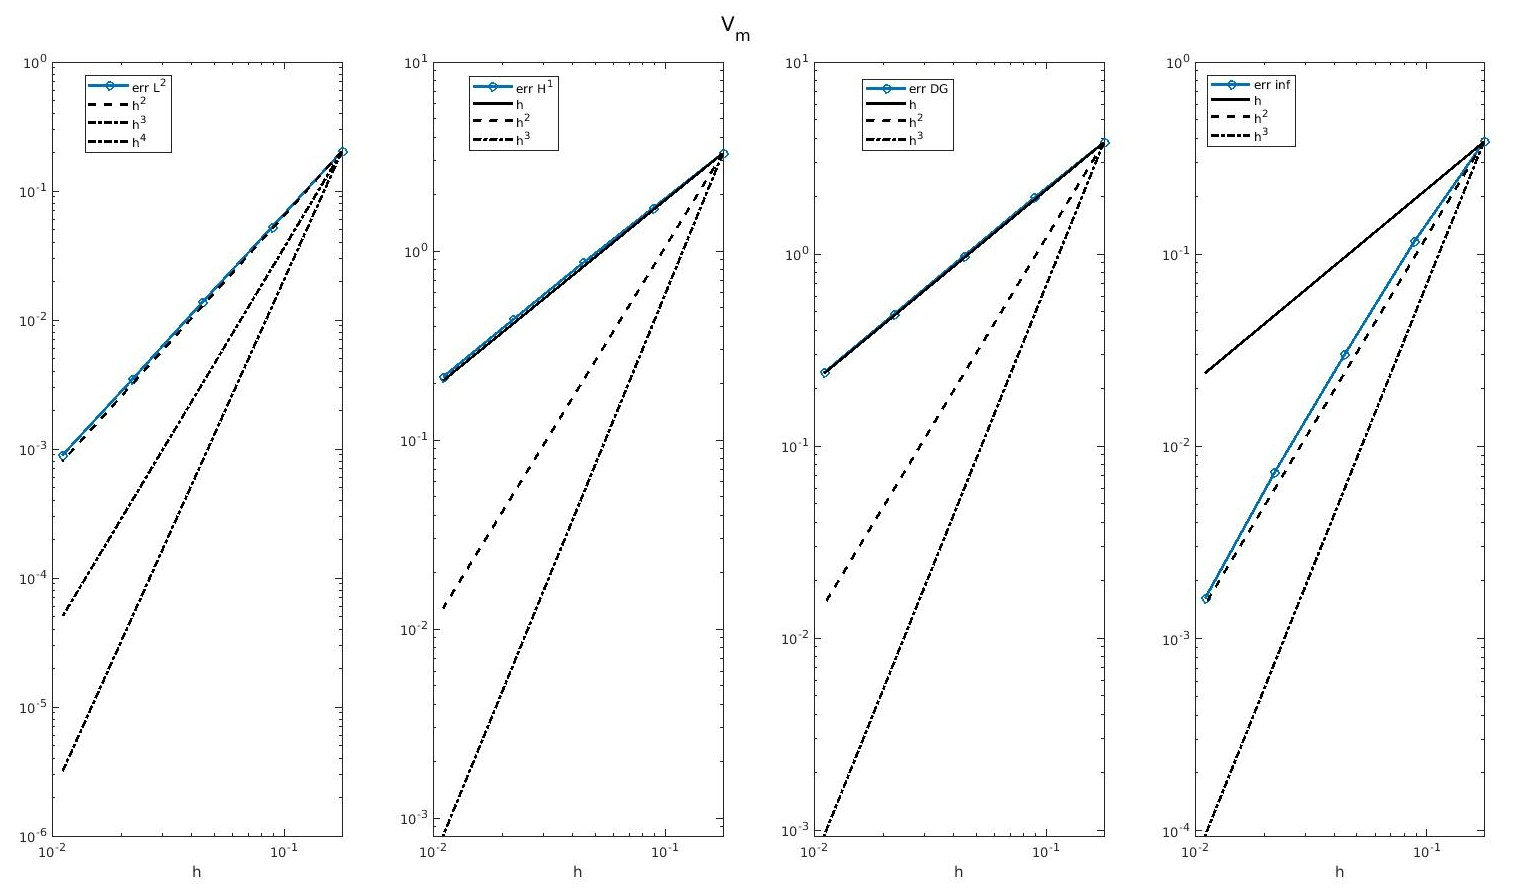
\includegraphics[width = 9cm]{./D1_Vm_1.jpg}
\caption{Trans-membrane potential  ($V_m$) with D1}
\end{subfigure}
\begin{subfigure}{0.5\textwidth}
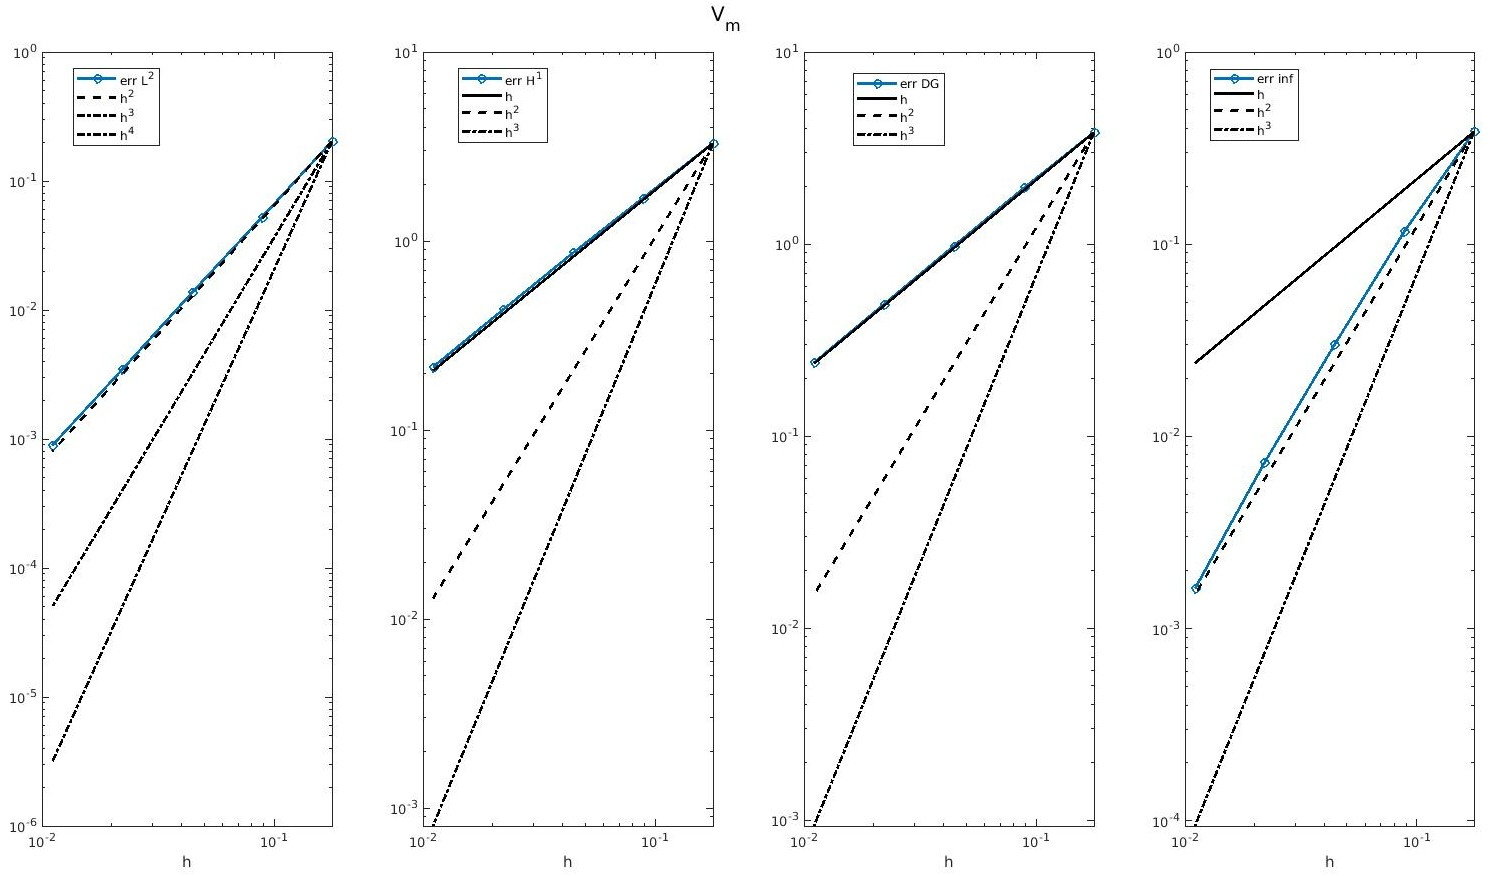
\includegraphics[width =9cm]{./P1_Vm_1.jpg}
\caption{Trans-membrane potential  ($V_m$) with P1}
\end{subfigure}
\begin{subfigure}{0.5\textwidth}
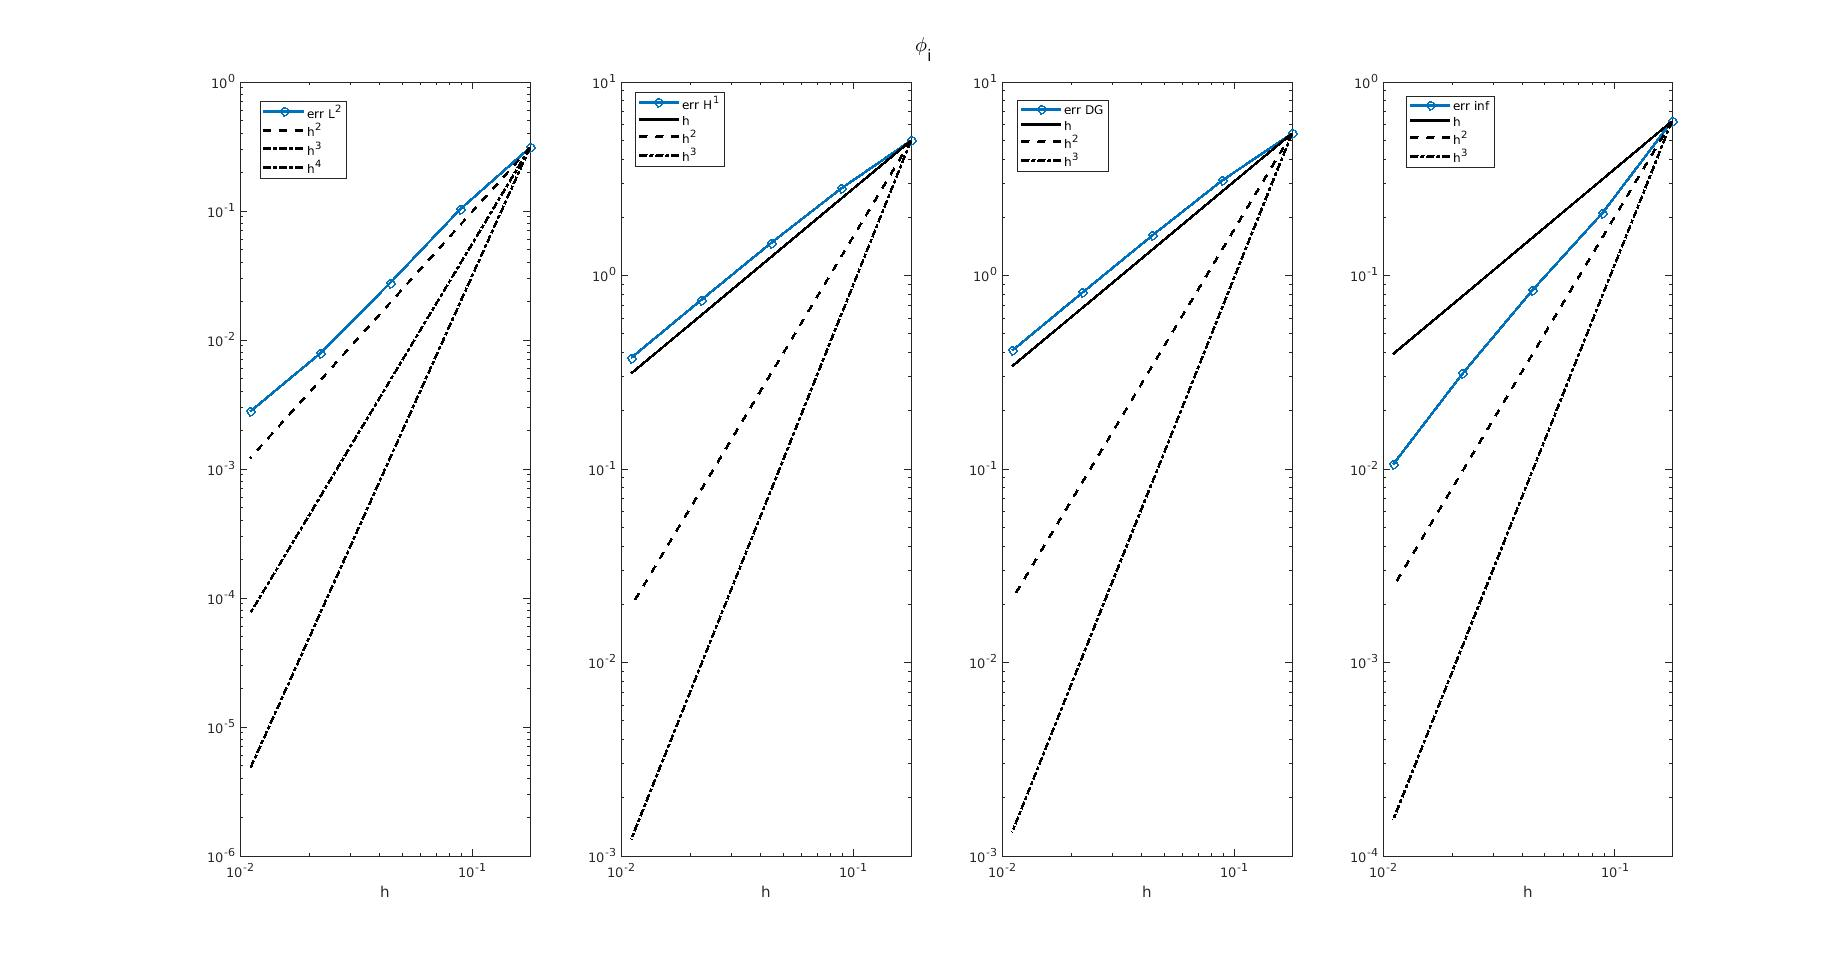
\includegraphics[width = 9cm]{./D1_Phii_1.jpg}
\caption{Intracellular potential ($\phi_i$) with D1}
\end{subfigure}
\hfill
\begin{subfigure}{0.5\textwidth}
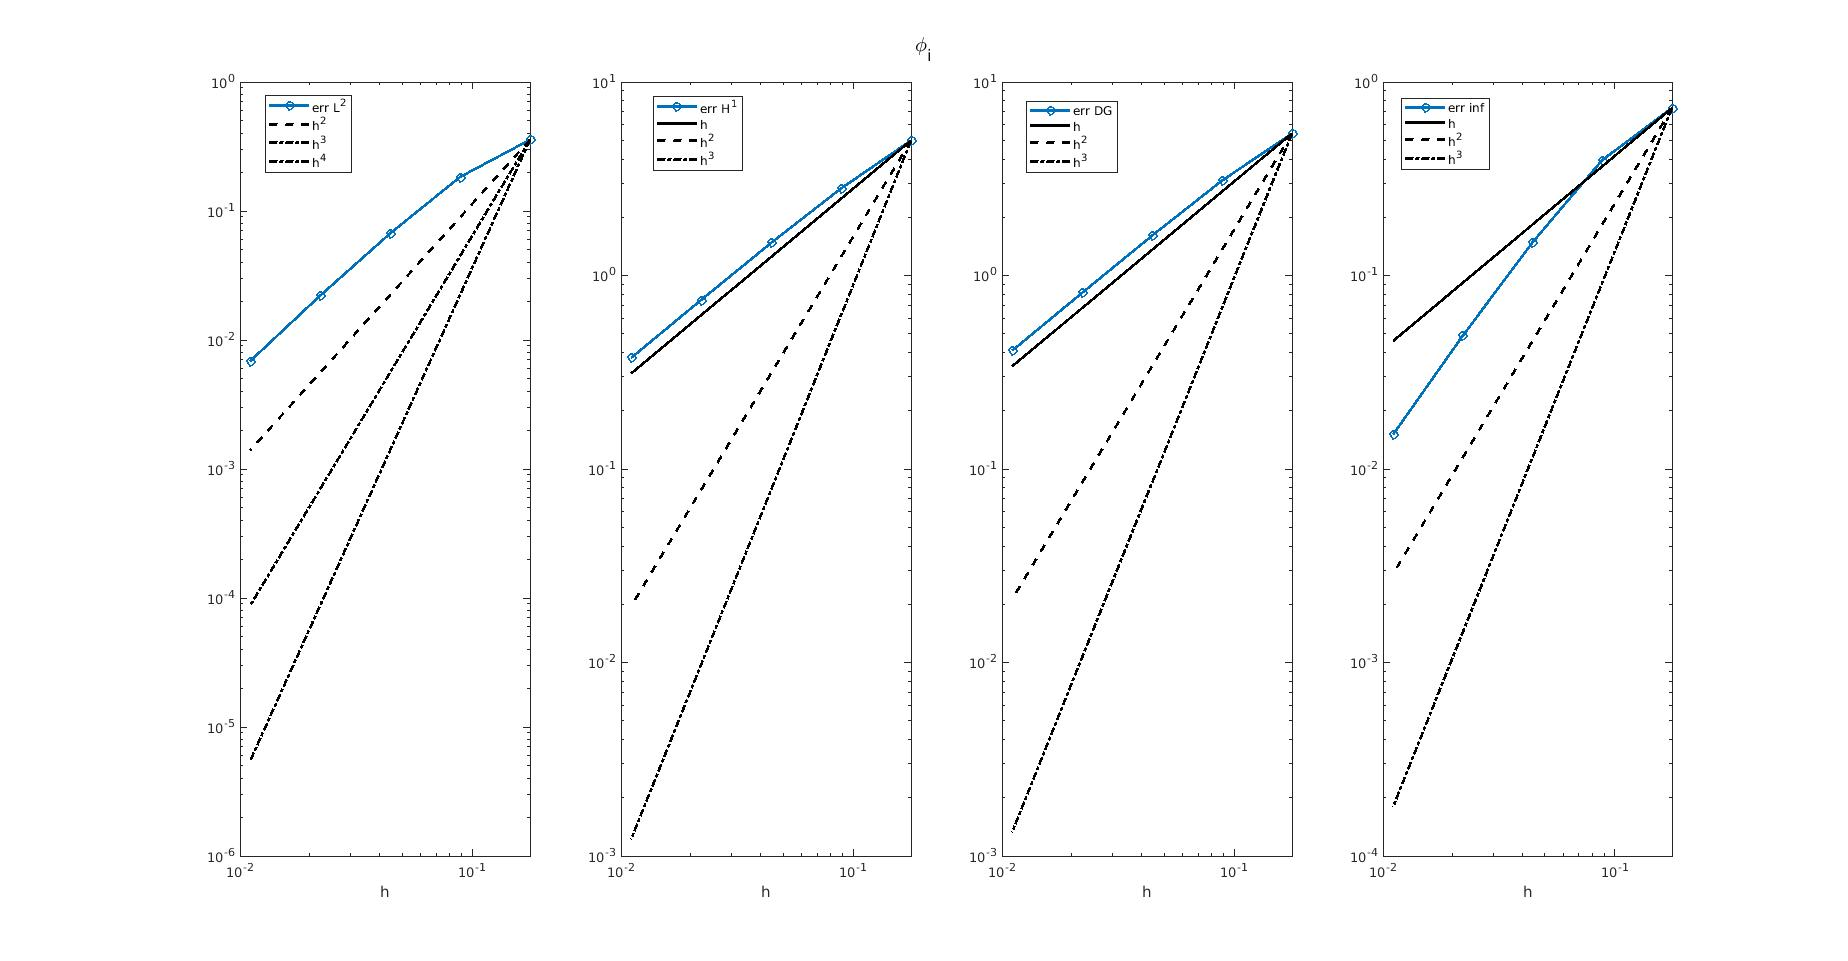
\includegraphics[width =9cm]{./P1_Phii_1.jpg}
\caption{Intracellular potential ($\phi_i$) with P1}
\end{subfigure}
\begin{subfigure}{0.5\textwidth}
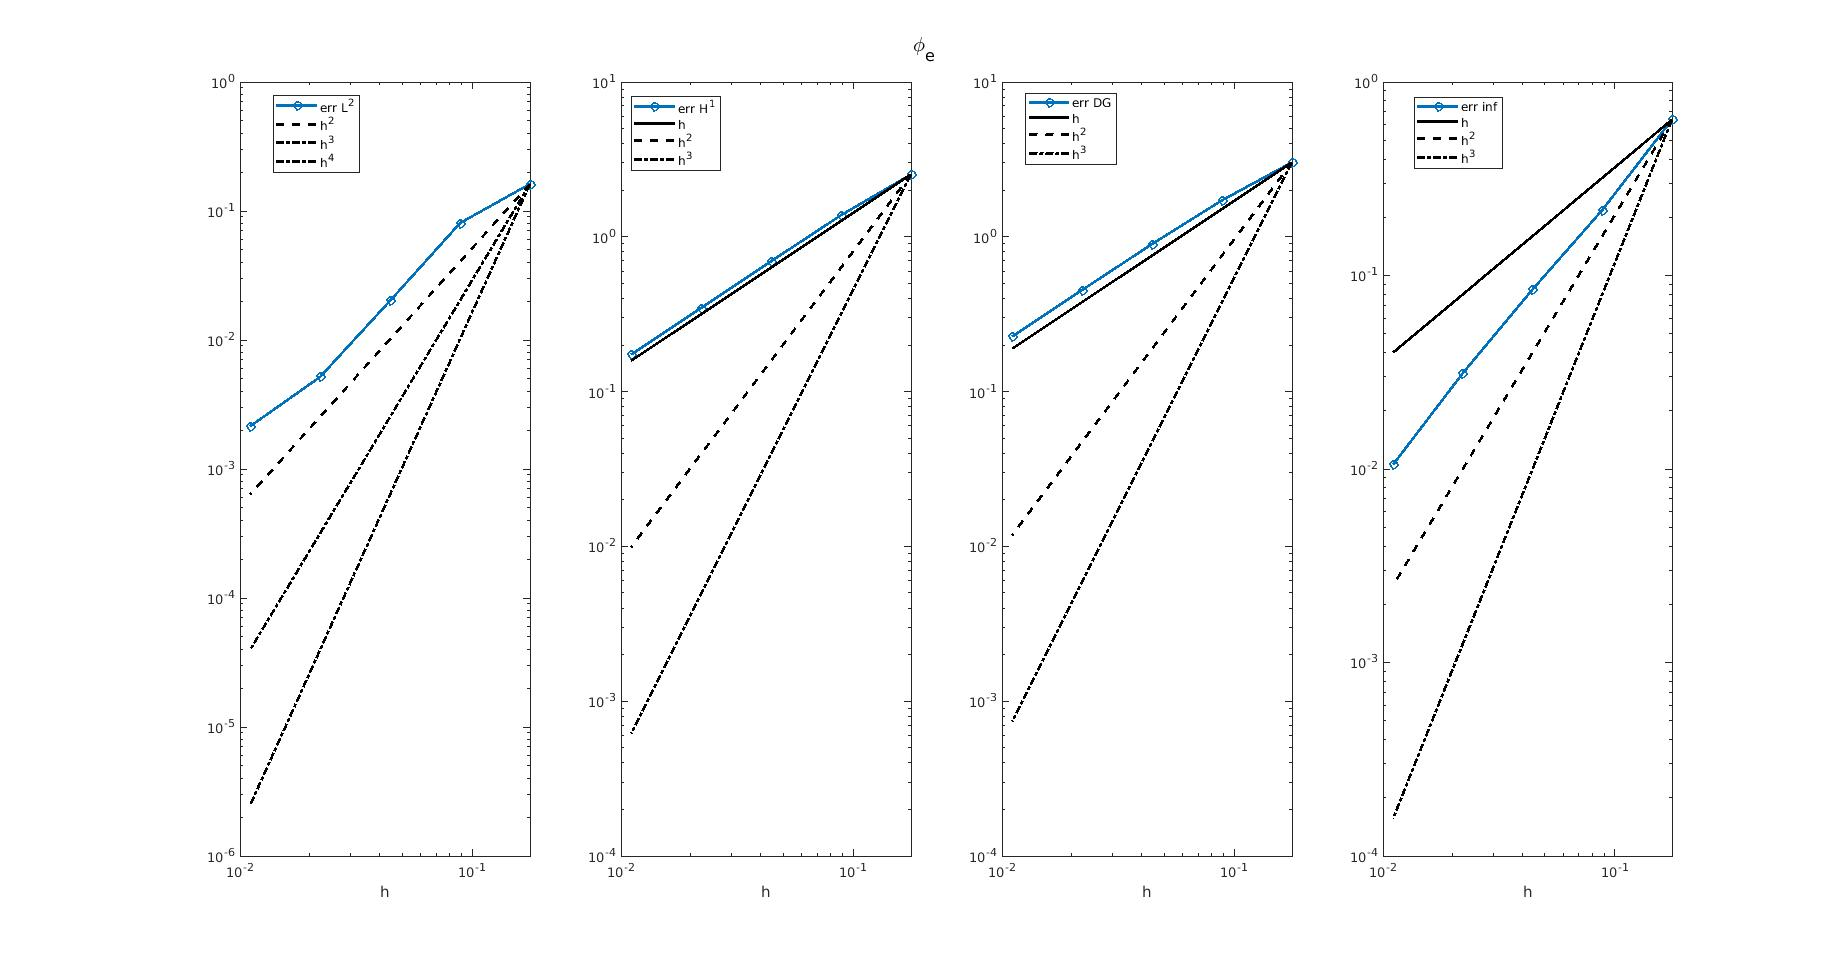
\includegraphics[width = 9cm]{./D1_Phie_1.jpg}
\caption{Extracellular potential ($\phi_e$) with D1}
\end{subfigure}
\begin{subfigure}{0.5\textwidth}
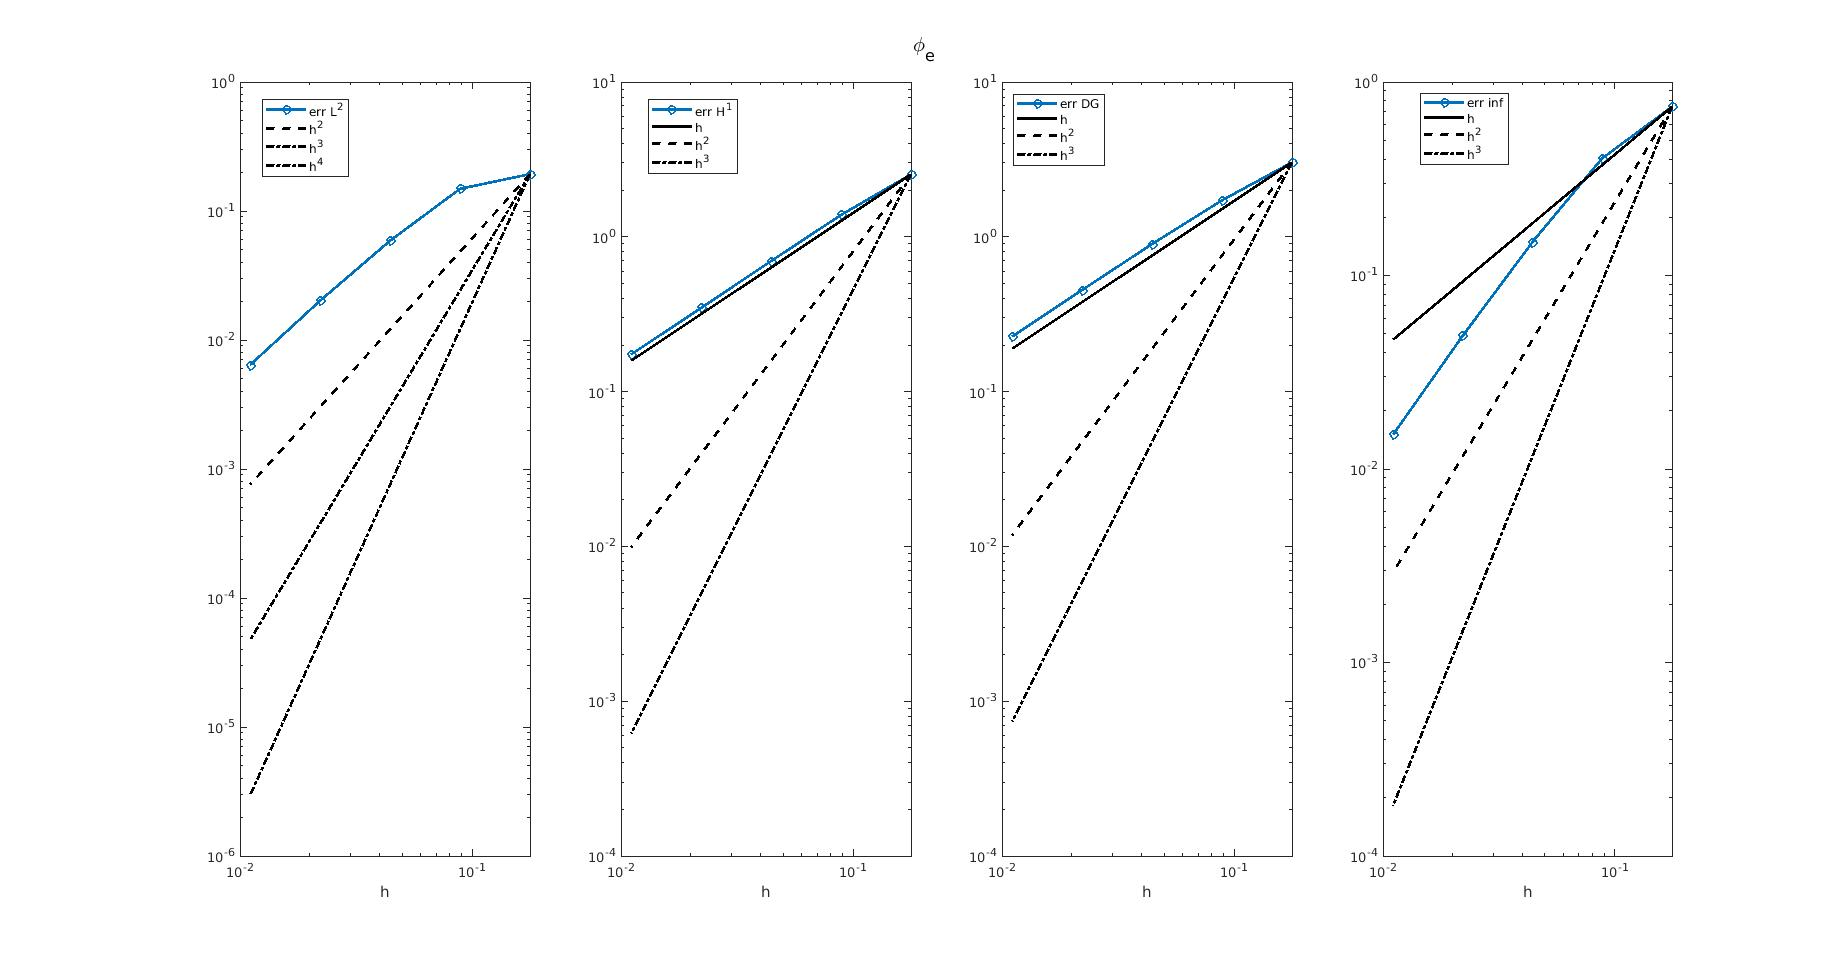
\includegraphics[width =9cm]{./P1_Phie_1.jpg}
\caption{Extracellular potential ($\phi_e$) with P1}
\end{subfigure}
\begin{subfigure}{0.5\textwidth}
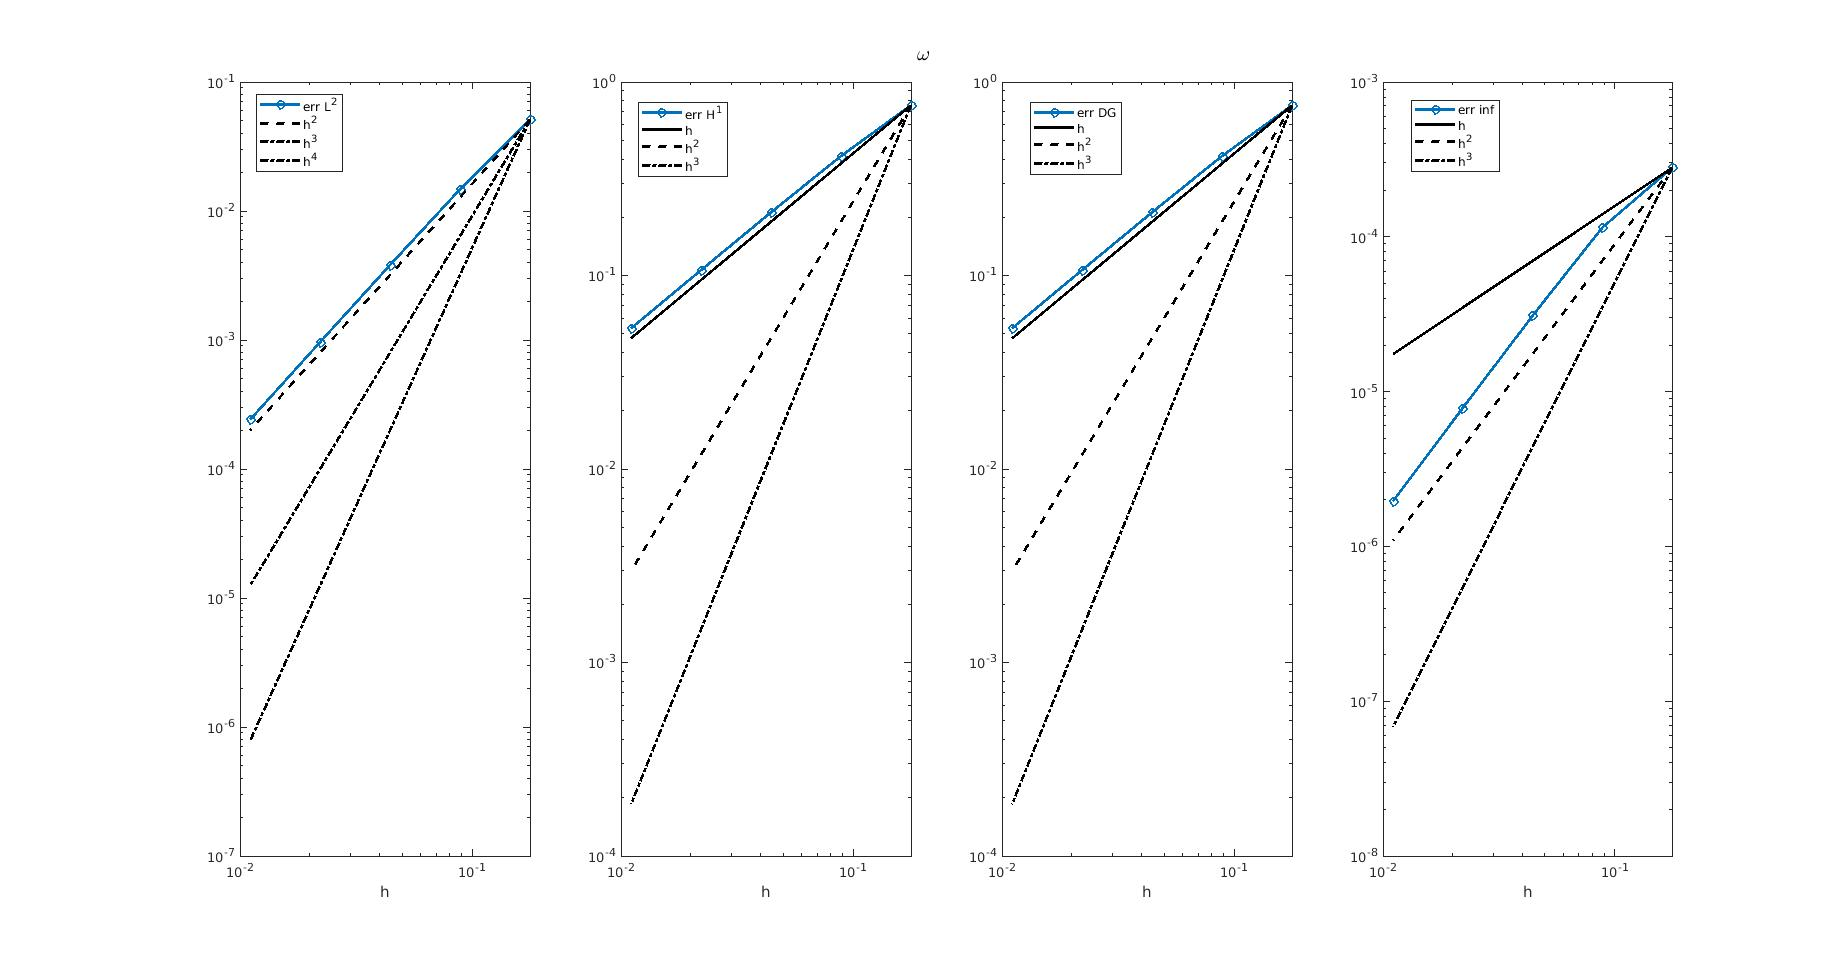
\includegraphics[width = 9cm]{./D1_w_1.jpg}
\caption{Gating variable ($w$) with D1}
\end{subfigure}
\begin{subfigure}{0.5\textwidth}
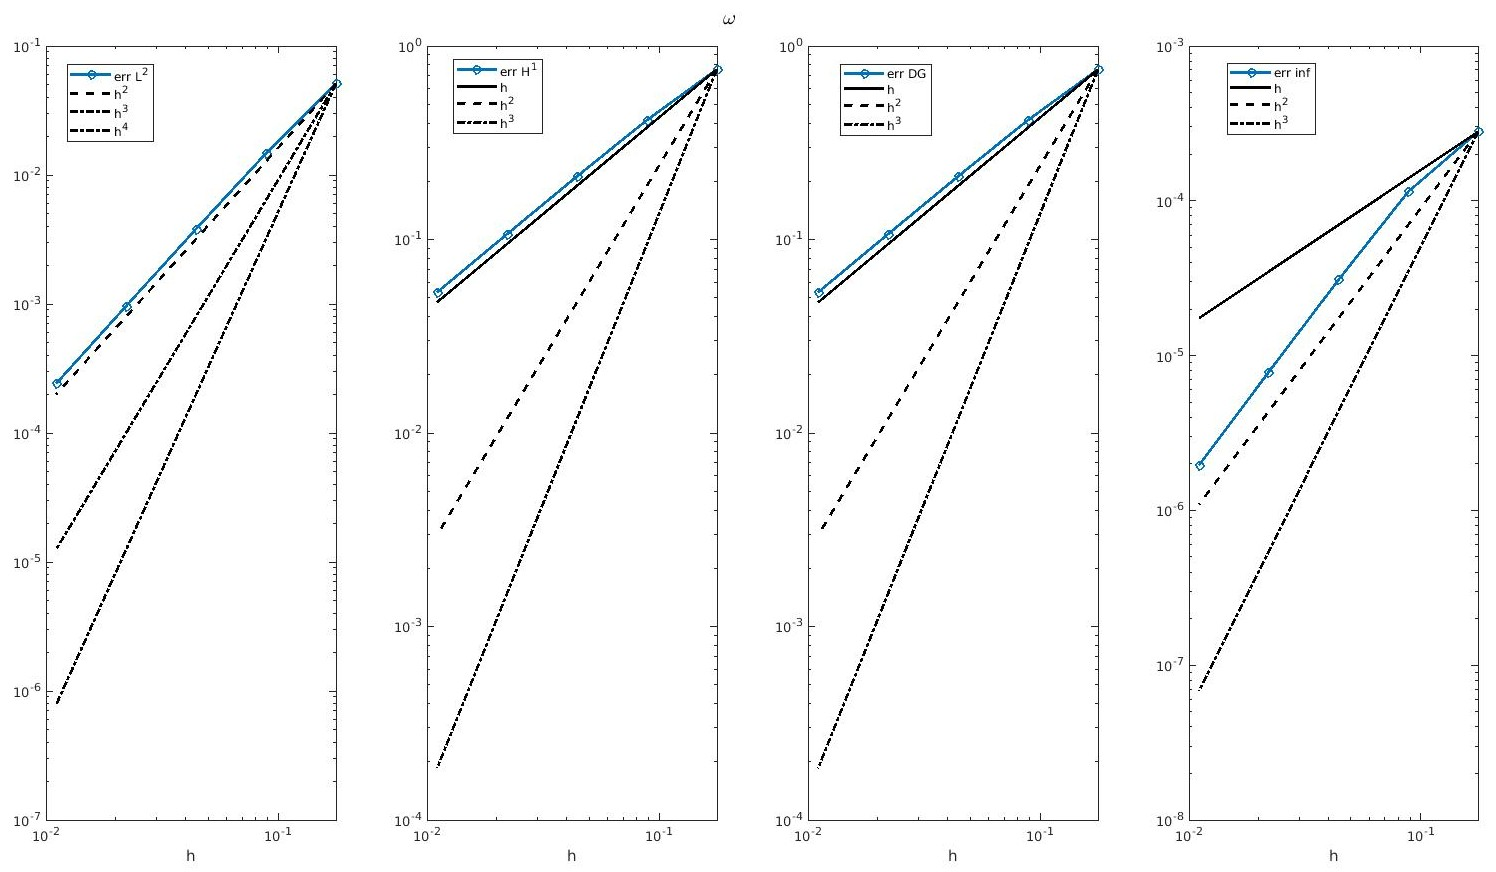
\includegraphics[width =9cm]{./P1_w_1.jpg}
\caption{Gating variable ($w$) with P1}
\end{subfigure}
\end{figure}
\restoregeometry
\newpage
\newgeometry{a4paper,top=1cm,bottom=2cm,left=1cm,right=1cm} 
\begin{figure}[h]\caption{Comparison between Dubiner and FEM with second order polynomials} \label{P2-D2_plot}
\begin{subfigure}{0.5\textwidth}
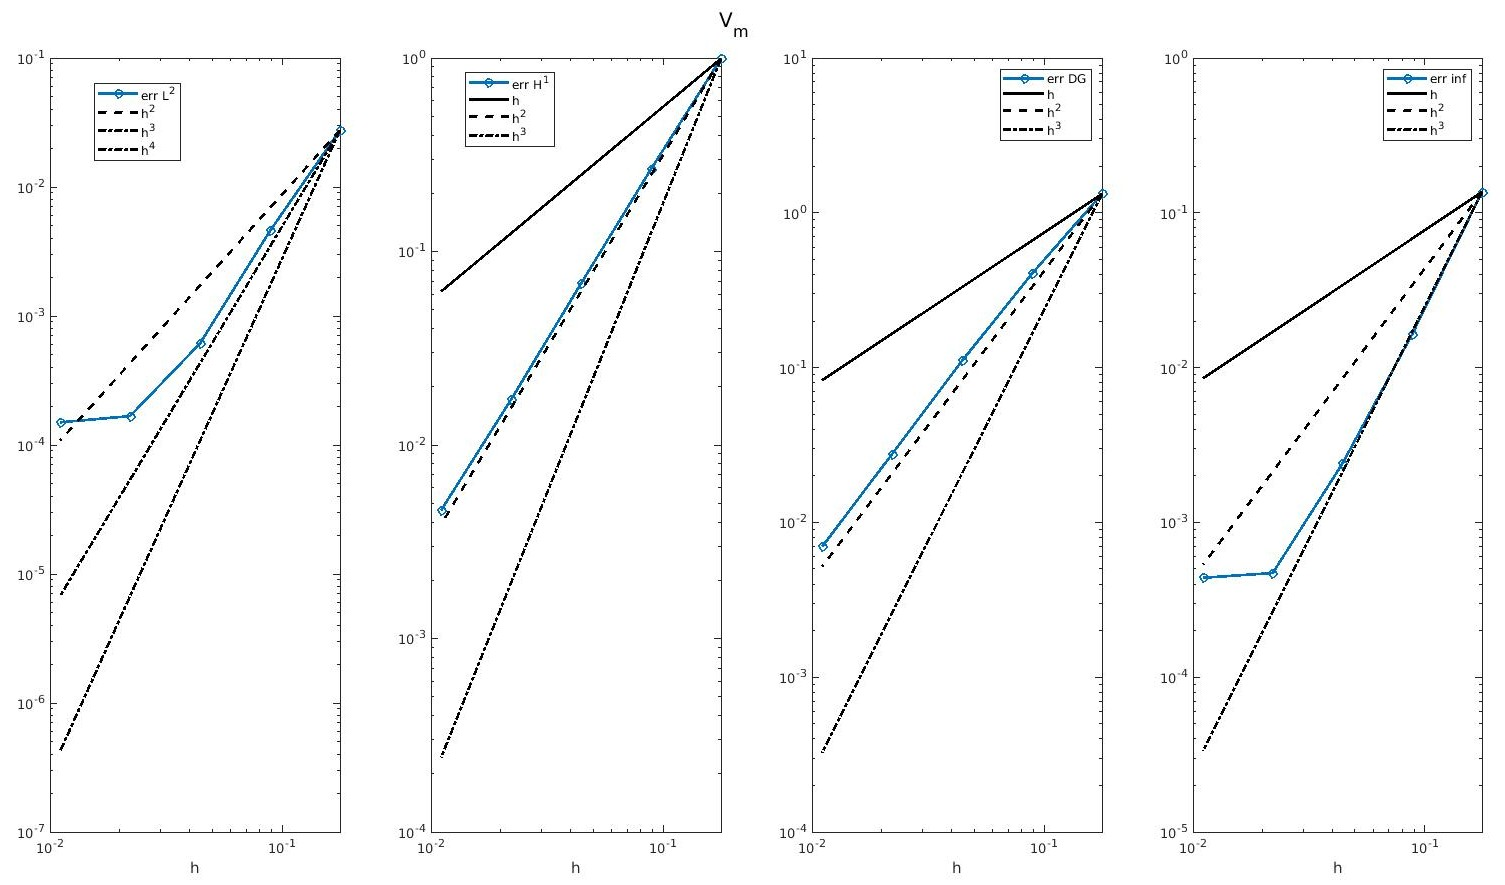
\includegraphics[width = 9cm]{./D2_Vm_1.jpg}
\caption{Trans-membrane potential  ($V_m$) with D2}
\end{subfigure}
\begin{subfigure}{0.5\textwidth}
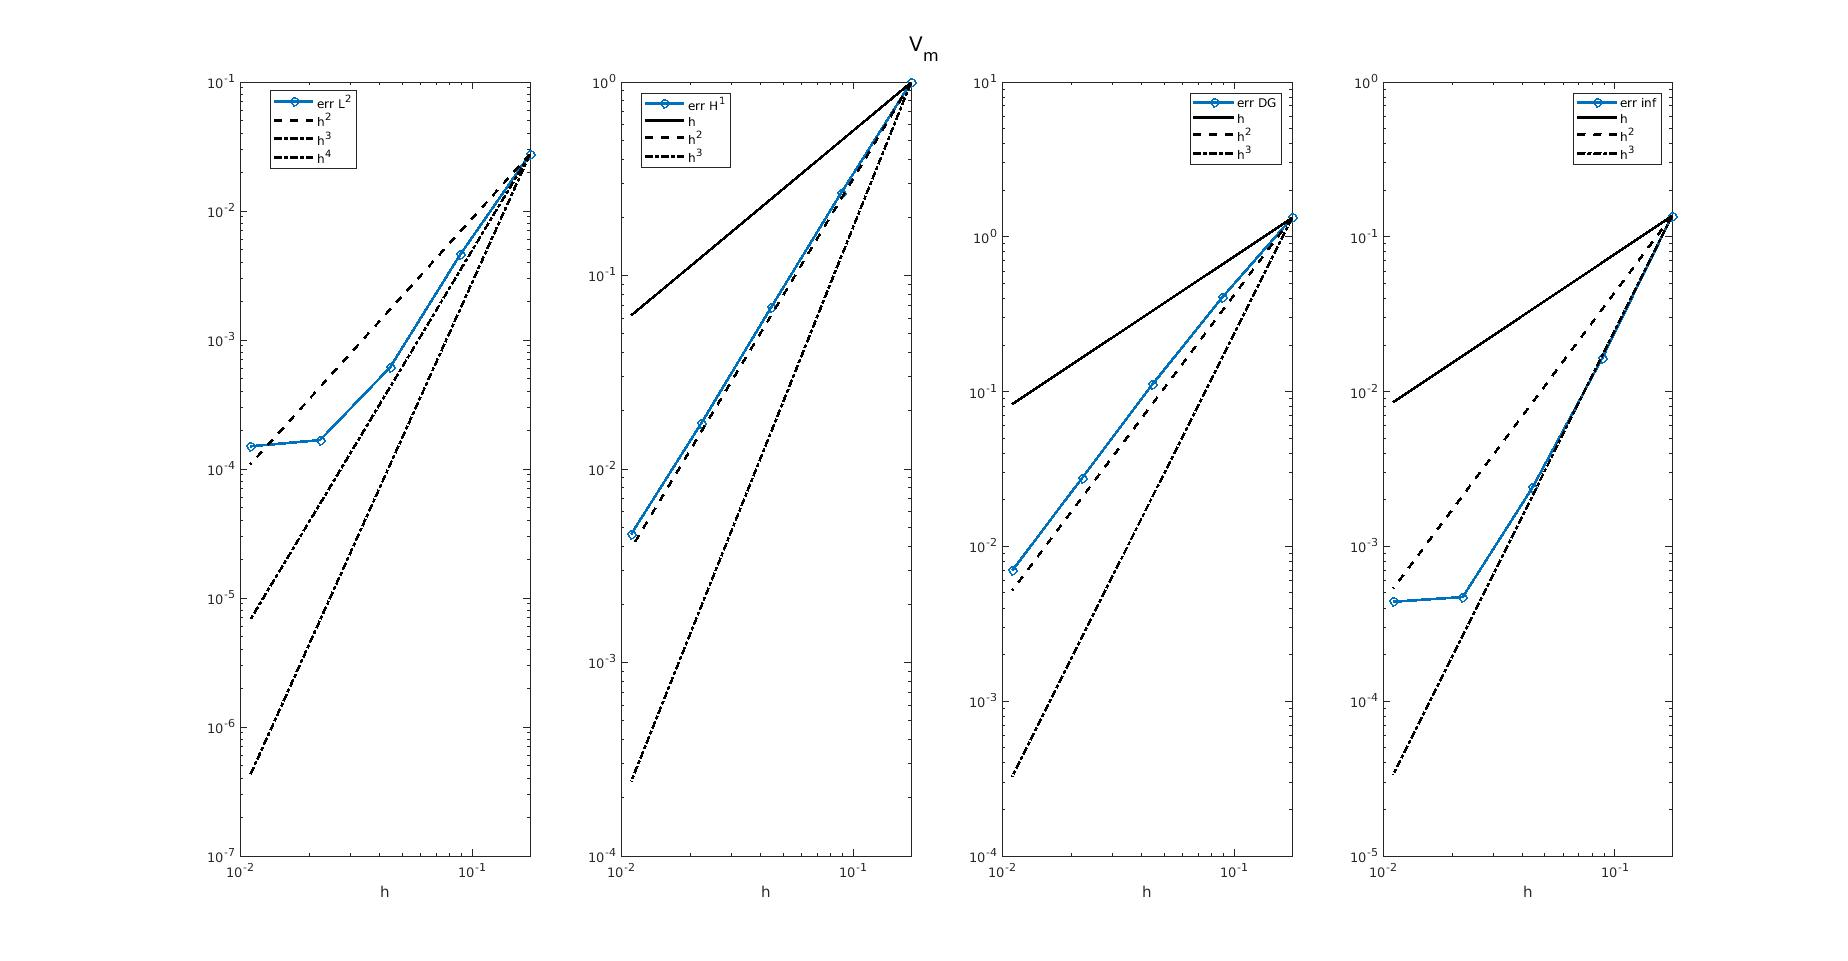
\includegraphics[width =9cm]{./P2_Vm_1.jpg}
\caption{Trans-membrane potential  ($V_m$) with P2}
\end{subfigure}
\begin{subfigure}{0.5\textwidth}
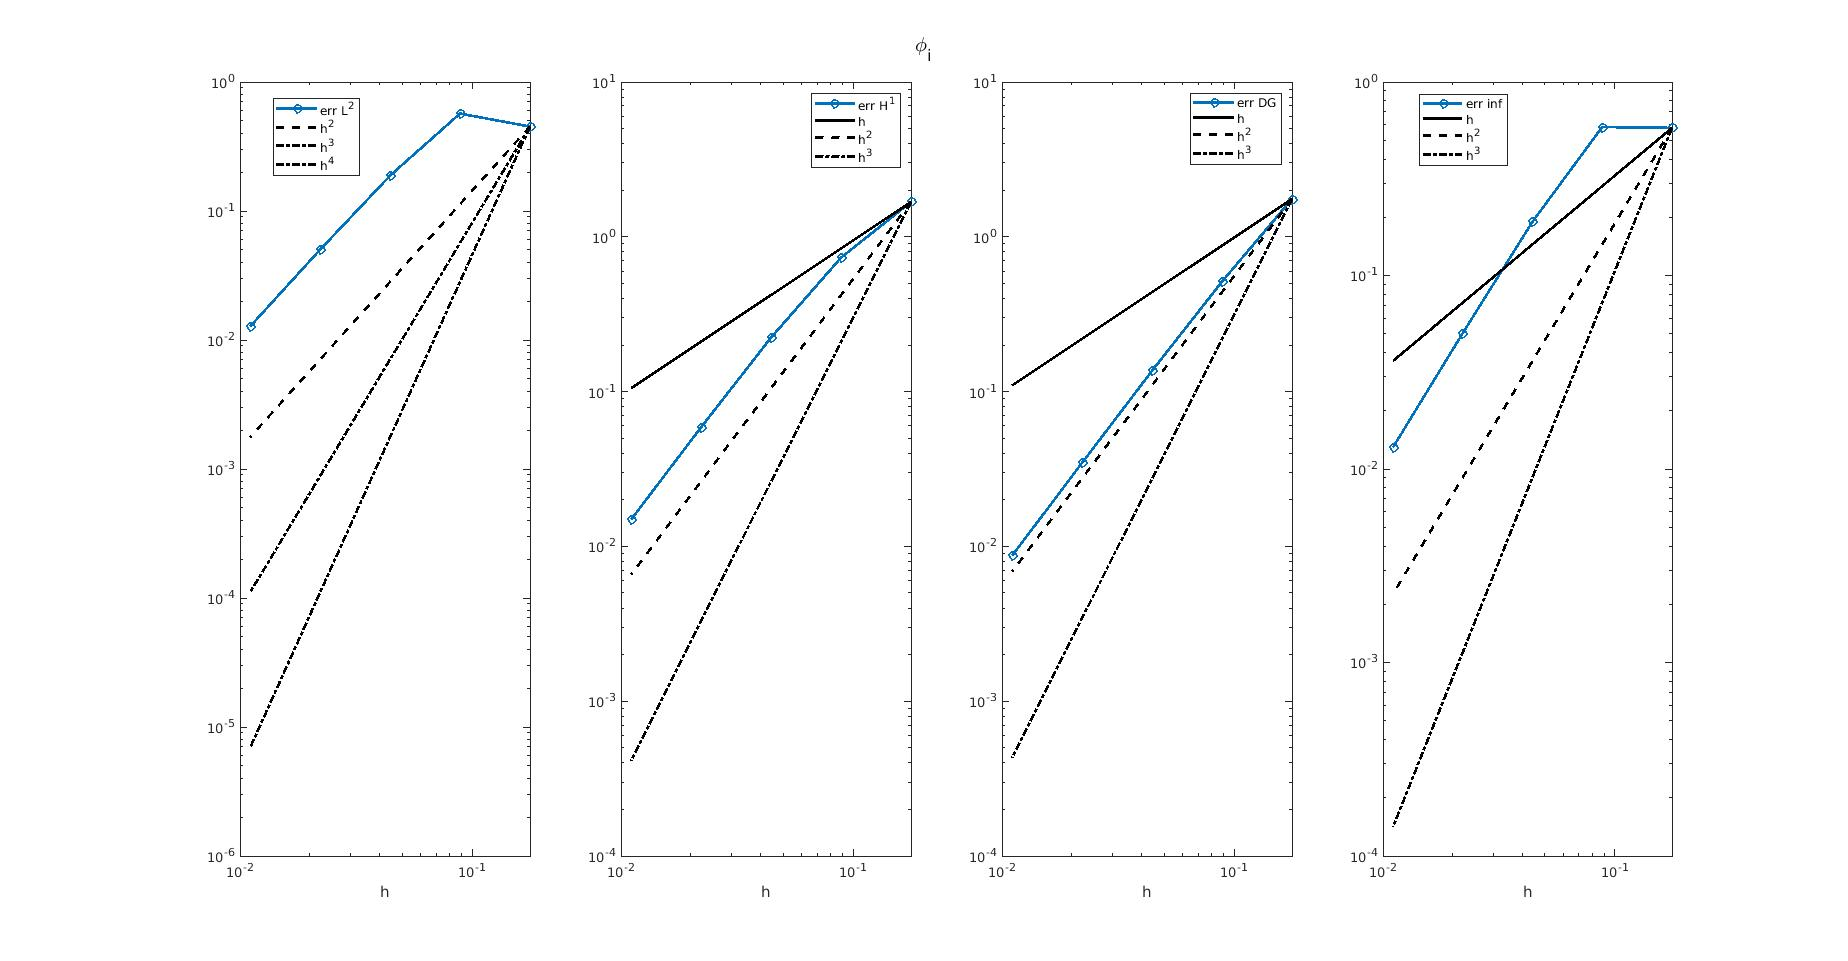
\includegraphics[width = 9cm]{./D2_Phii_1.jpg}
\caption{Intracellular potential ($\phi_i$) with D2}
\end{subfigure}
\begin{subfigure}{0.5\textwidth}
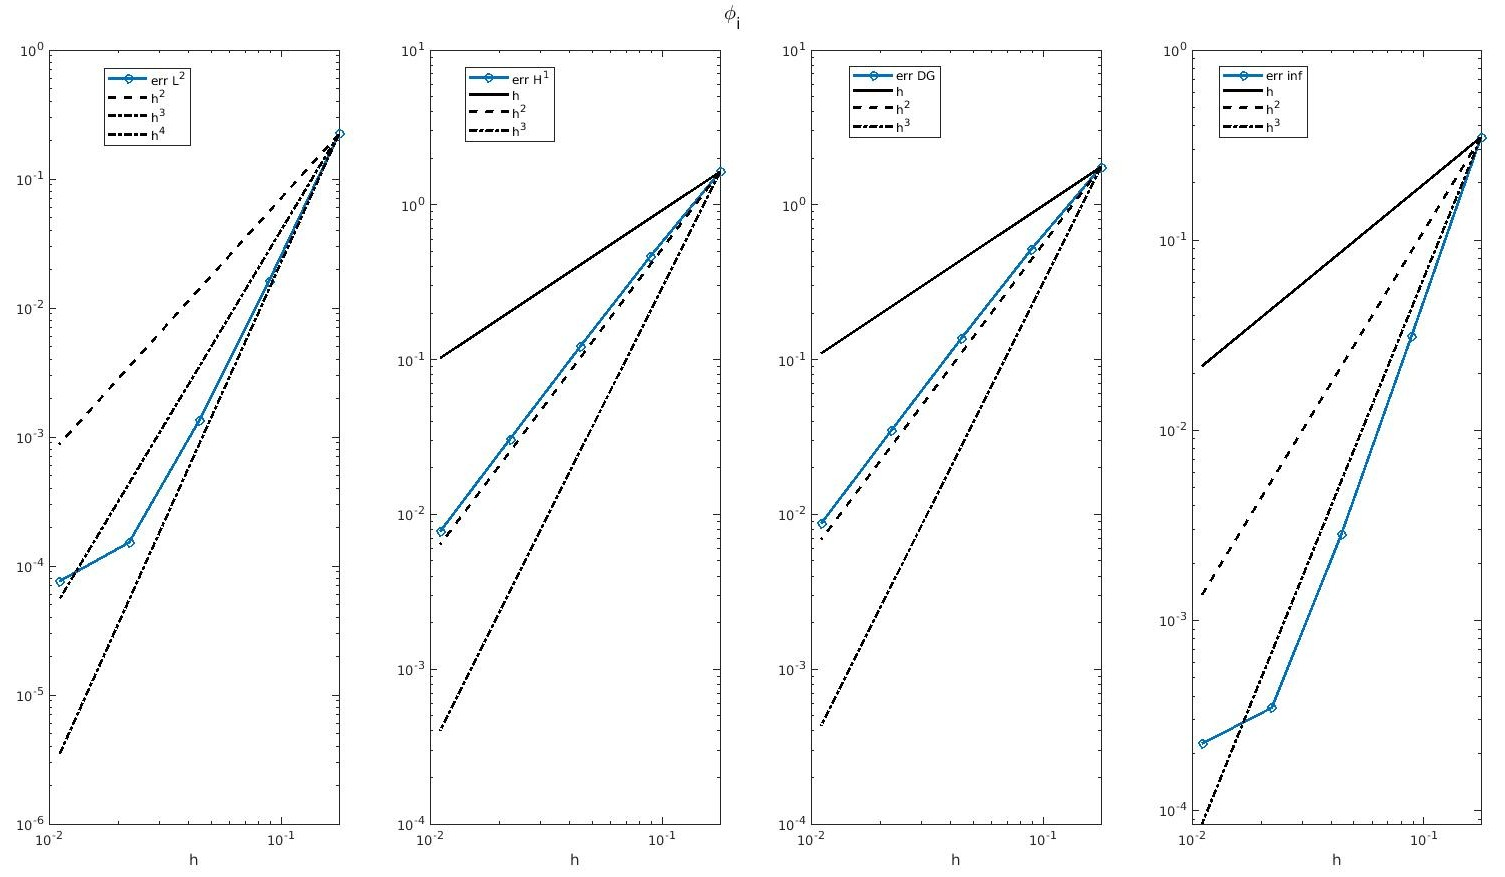
\includegraphics[width =9cm]{./P2_Phii_1.jpg}
\caption{Intracellular potential ($\phi_i$) with P2}
\end{subfigure}
\begin{subfigure}{0.5\textwidth}
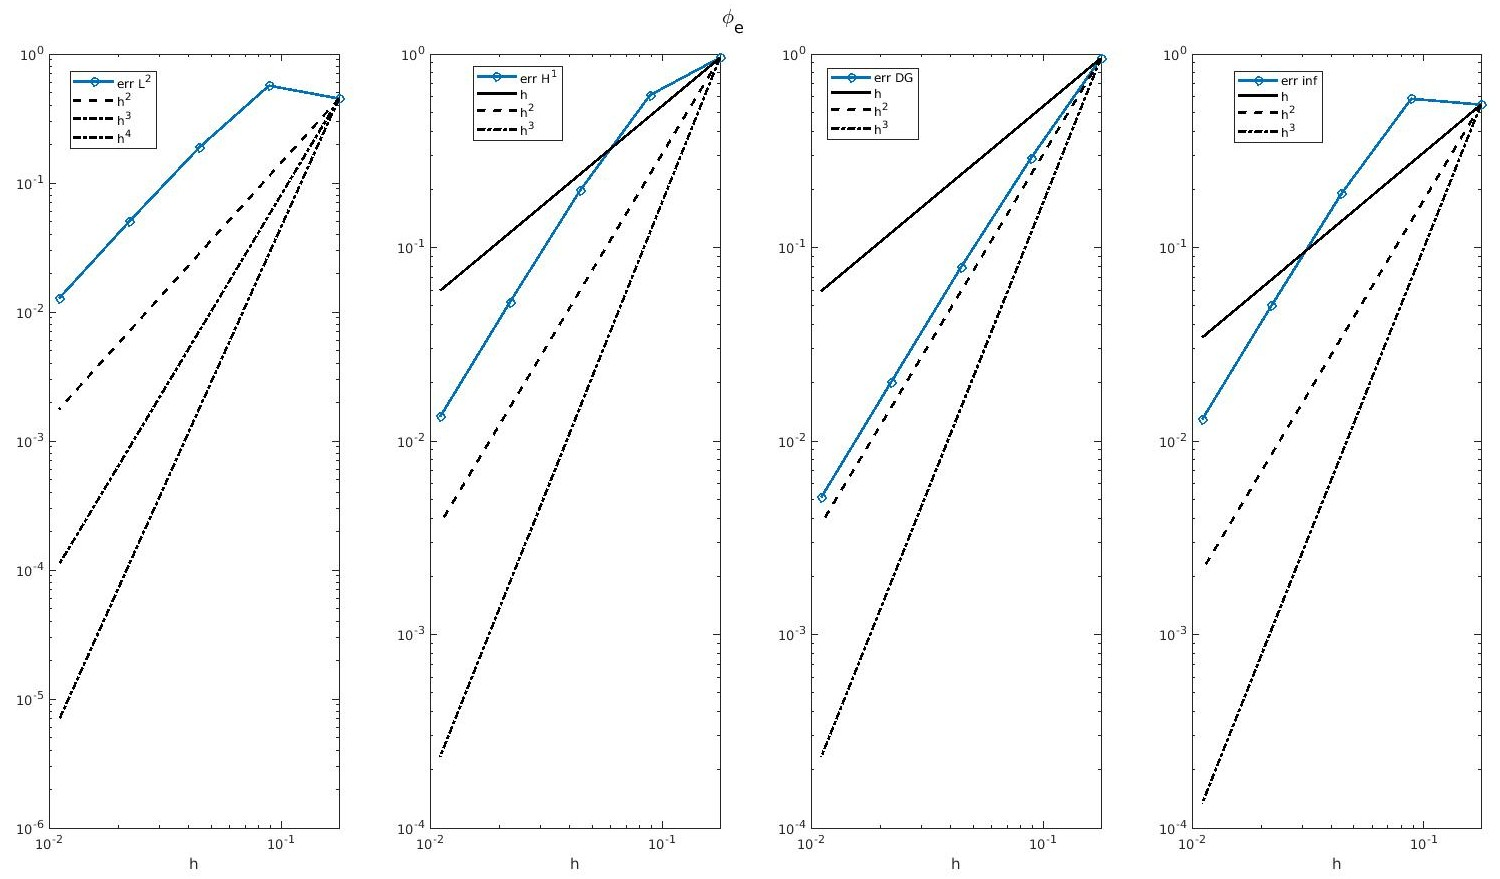
\includegraphics[width = 9cm]{./D2_Phie_1.jpg}
\caption{Extracellular potential ($\phi_e$) with D2}
\end{subfigure}
\begin{subfigure}{0.5\textwidth}
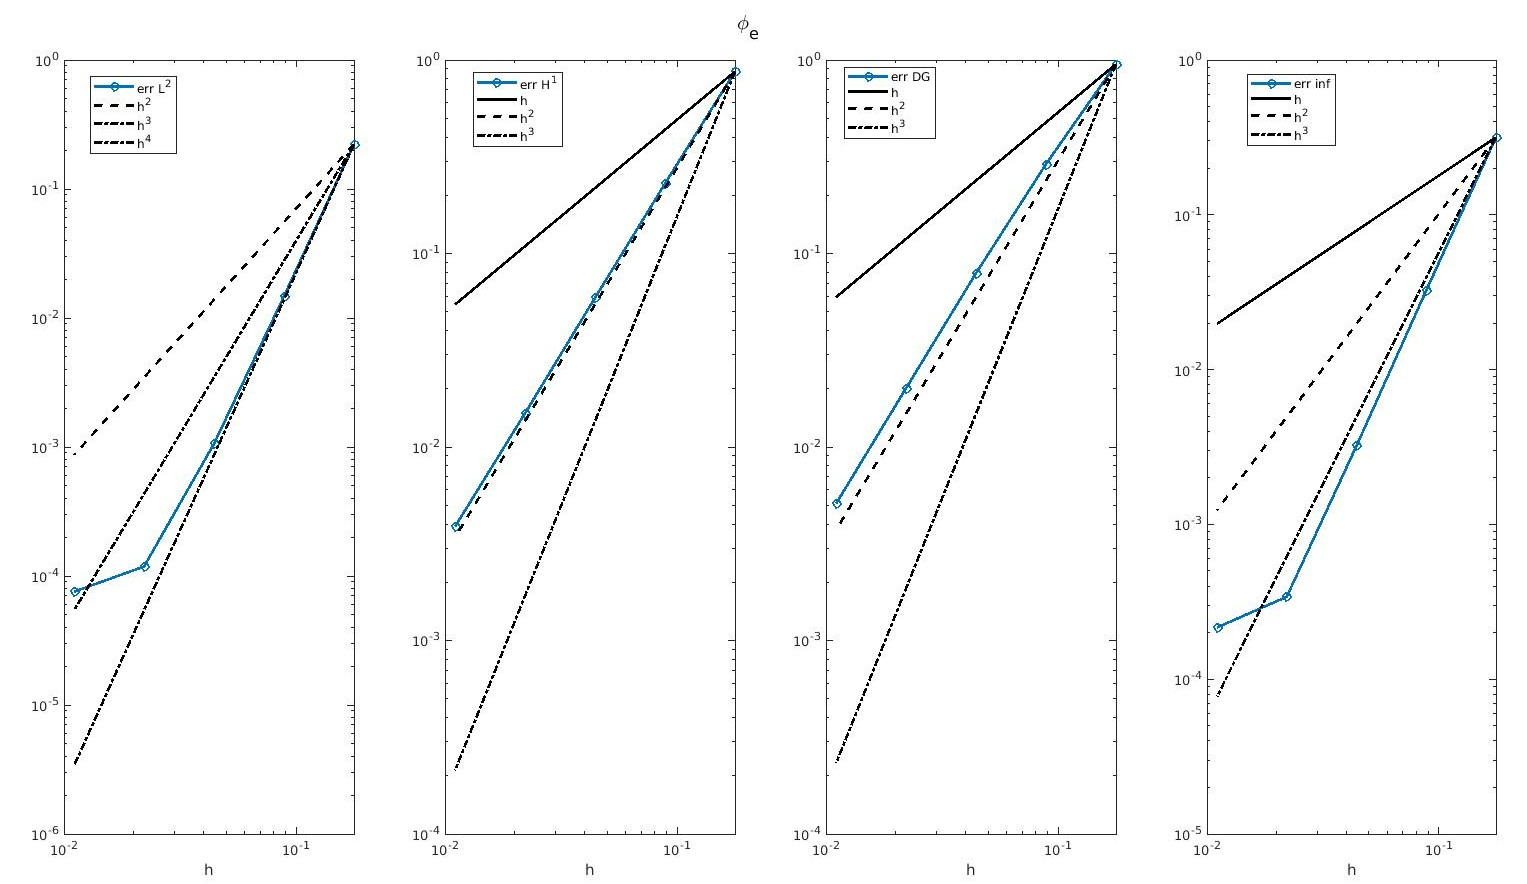
\includegraphics[width =9cm]{./P2_Phie_1.jpg}
\caption{Extracellular potential ($\phi_e$) with P2}
\end{subfigure}
\begin{subfigure}{0.5\textwidth}
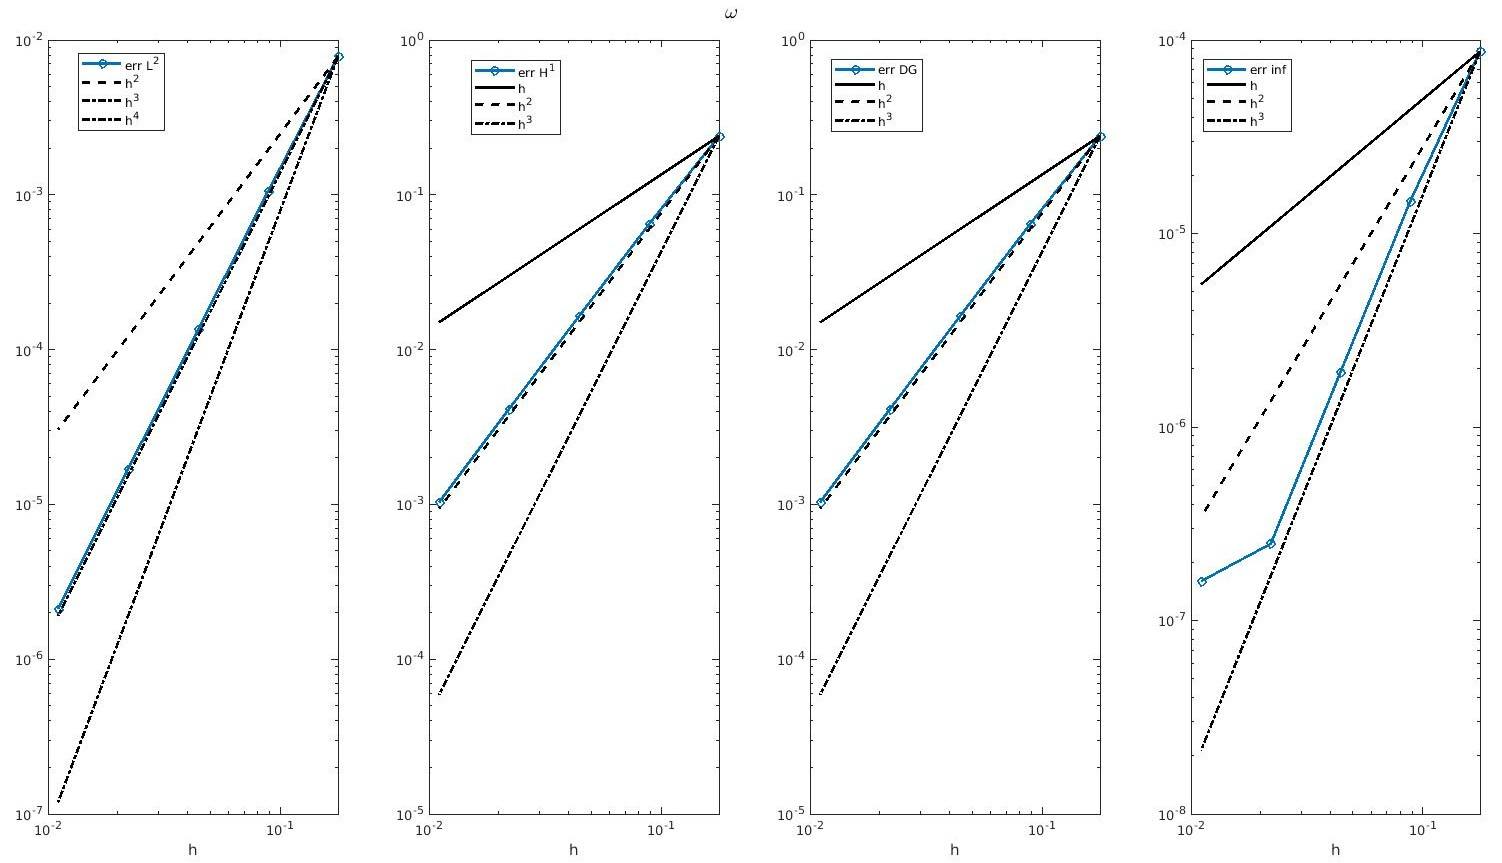
\includegraphics[width = 9cm]{./D2_w_1.jpg}
\caption{Gating variable ($w$) with D2}
\end{subfigure}
\begin{subfigure}{0.5\textwidth}
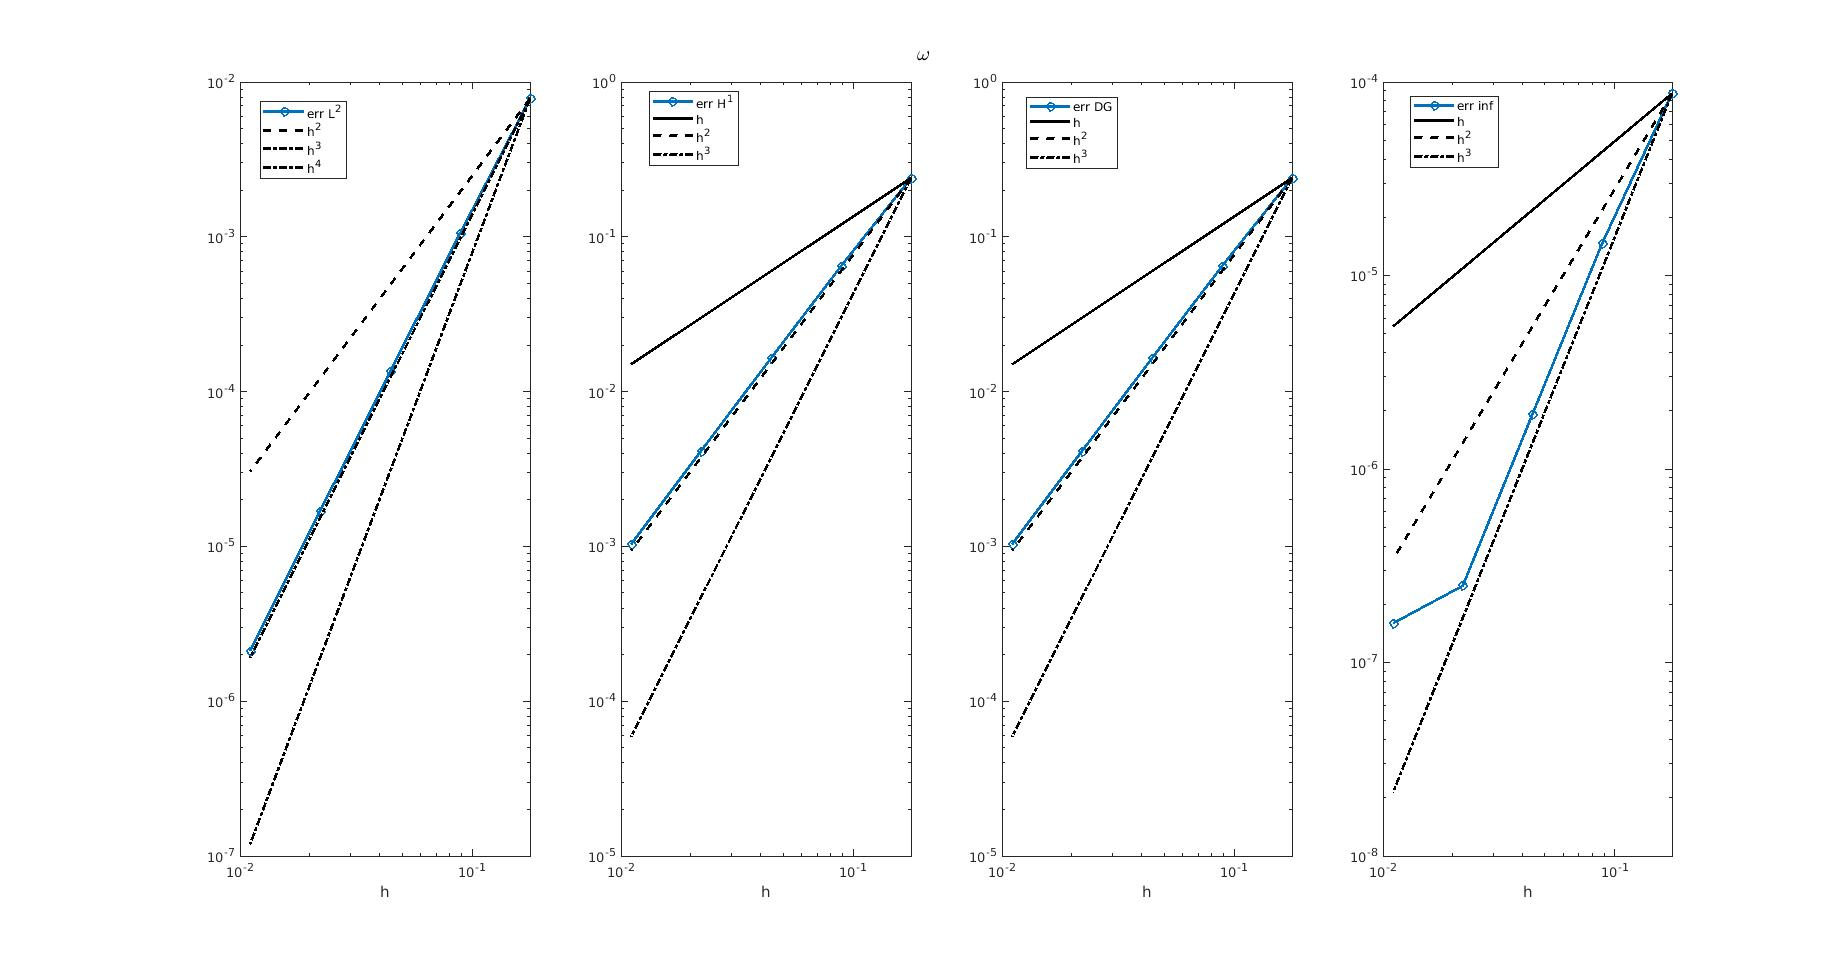
\includegraphics[width =9cm]{./P2_w_1.jpg}
\caption{Gating variable ($w$) with P2}
\end{subfigure}
\end{figure}
\restoregeometry
\newpage
\newgeometry{a4paper,top=1cm,bottom=2cm,left=1cm,right=1cm} 
\begin{figure}[h] \caption{Comparison between Dubiner and FEM with third order polynomials} \label{P3-D3_plot}
\begin{subfigure}{0.5\textwidth}
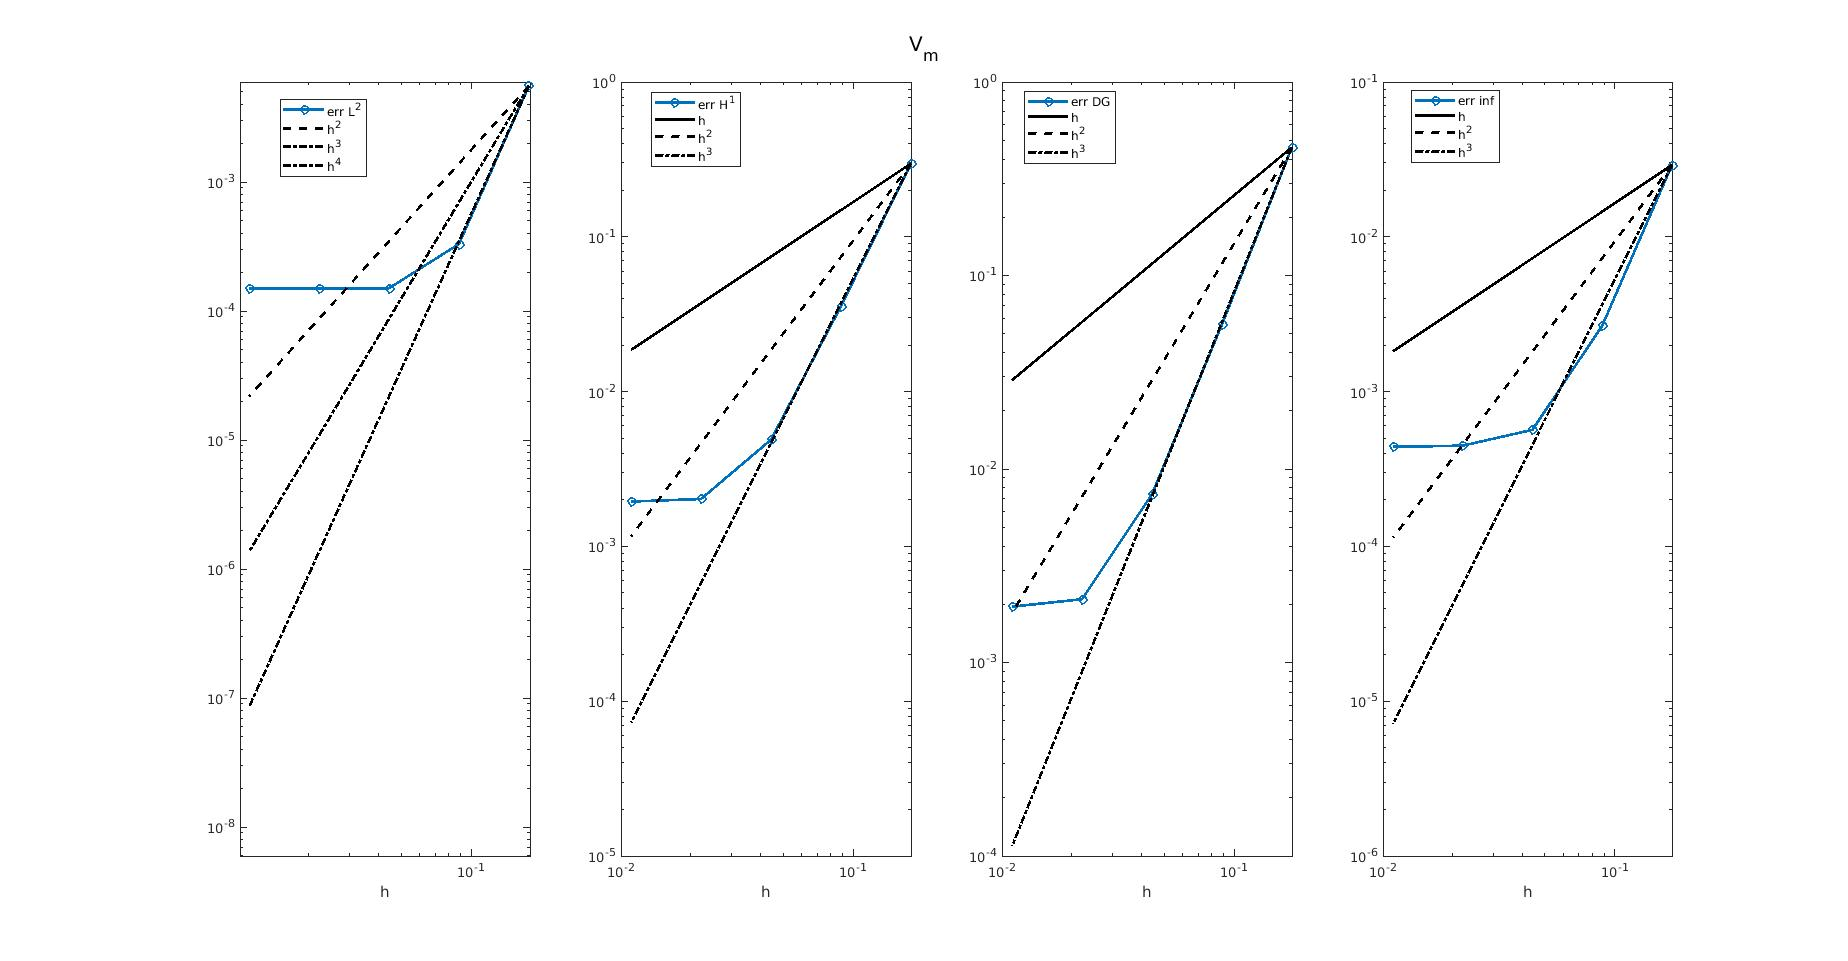
\includegraphics[width = 9cm]{./D3_Vm_1.jpg}
\caption{Trans-membrane potential ($V_m$) with D3}
\end{subfigure}
\begin{subfigure}{0.5\textwidth}
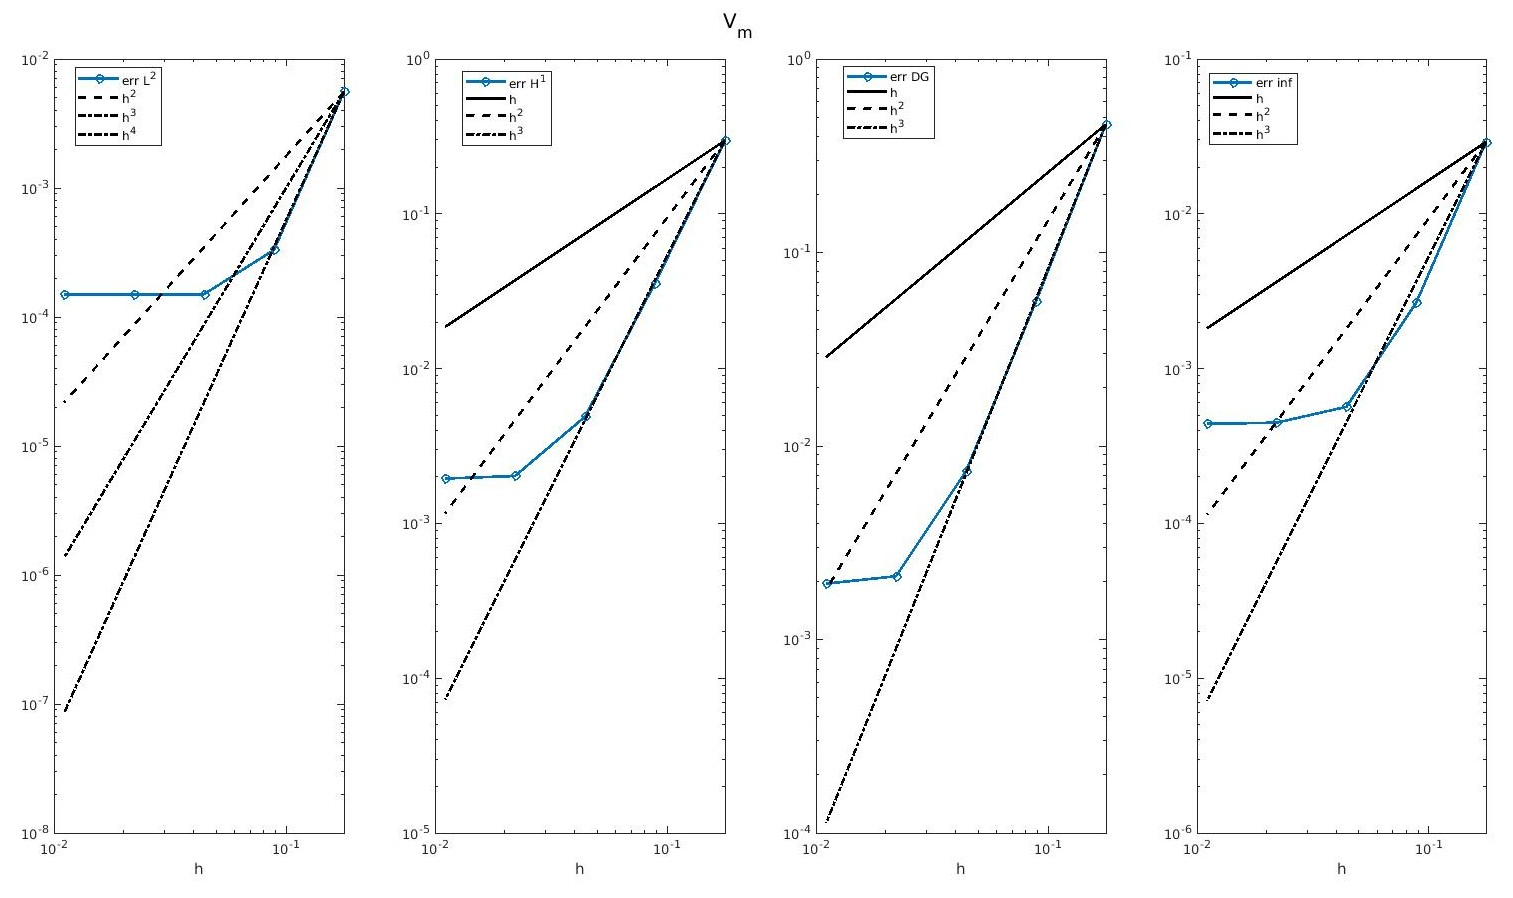
\includegraphics[width =9cm]{./P3_Vm_1.jpg}
\caption{Trans-membrane potential  ($V_m$) with P3}
\end{subfigure}
\begin{subfigure}{0.5\textwidth}
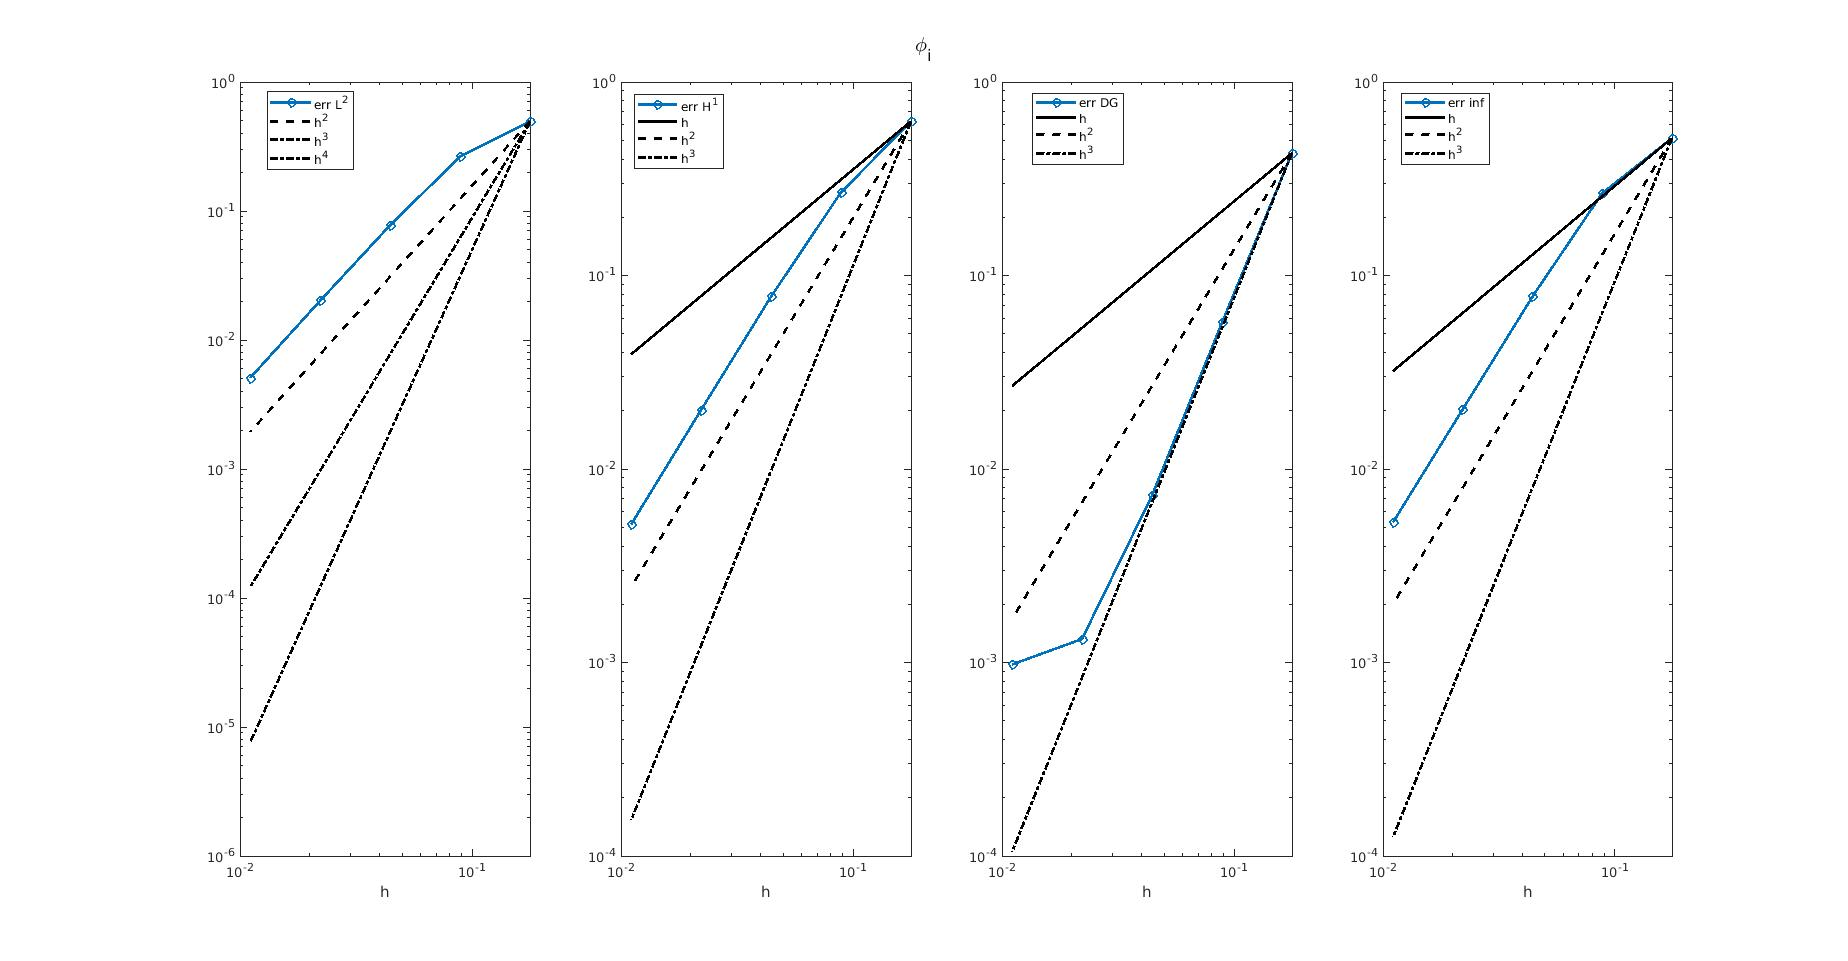
\includegraphics[width = 9cm]{./D3_Phii_1.jpg}
\caption{Intracellular potential ($\phi_i$) with D3}
\end{subfigure}
\begin{subfigure}{0.5\textwidth}
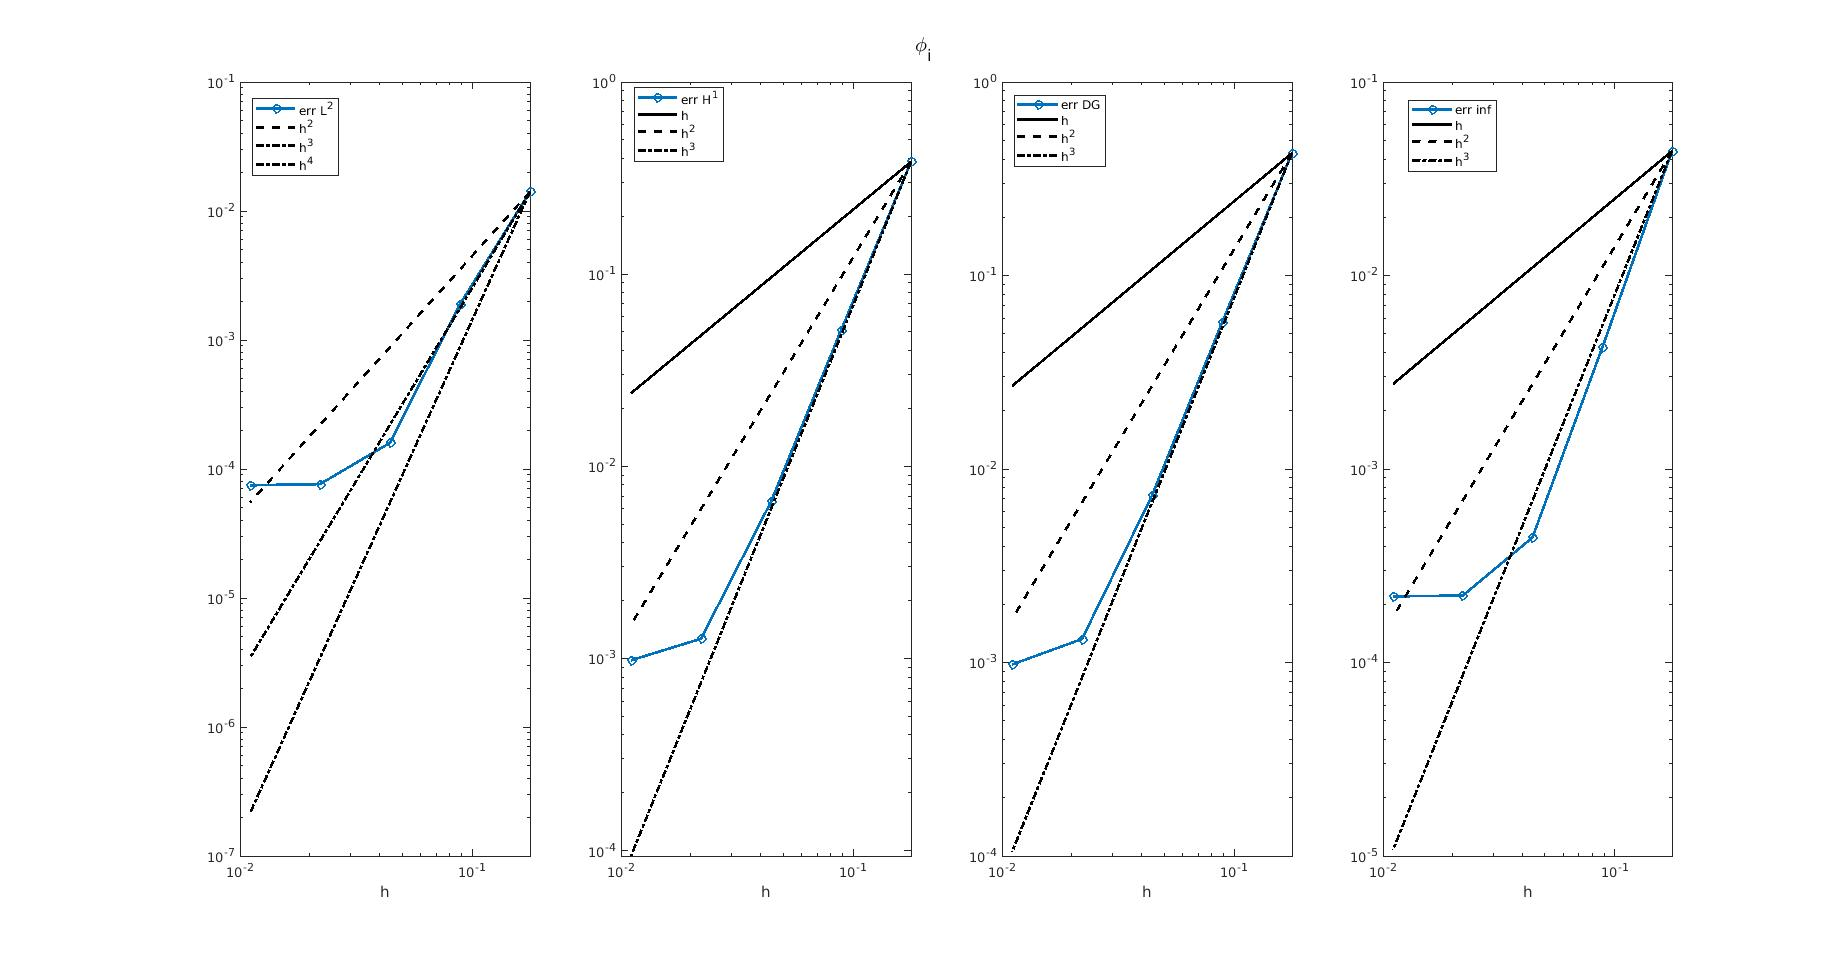
\includegraphics[width =9cm]{./P3_Phii_1.jpg}
\caption{Intracellular potential ($\phi_i$) with P3}
\end{subfigure}
\begin{subfigure}{0.5\textwidth}
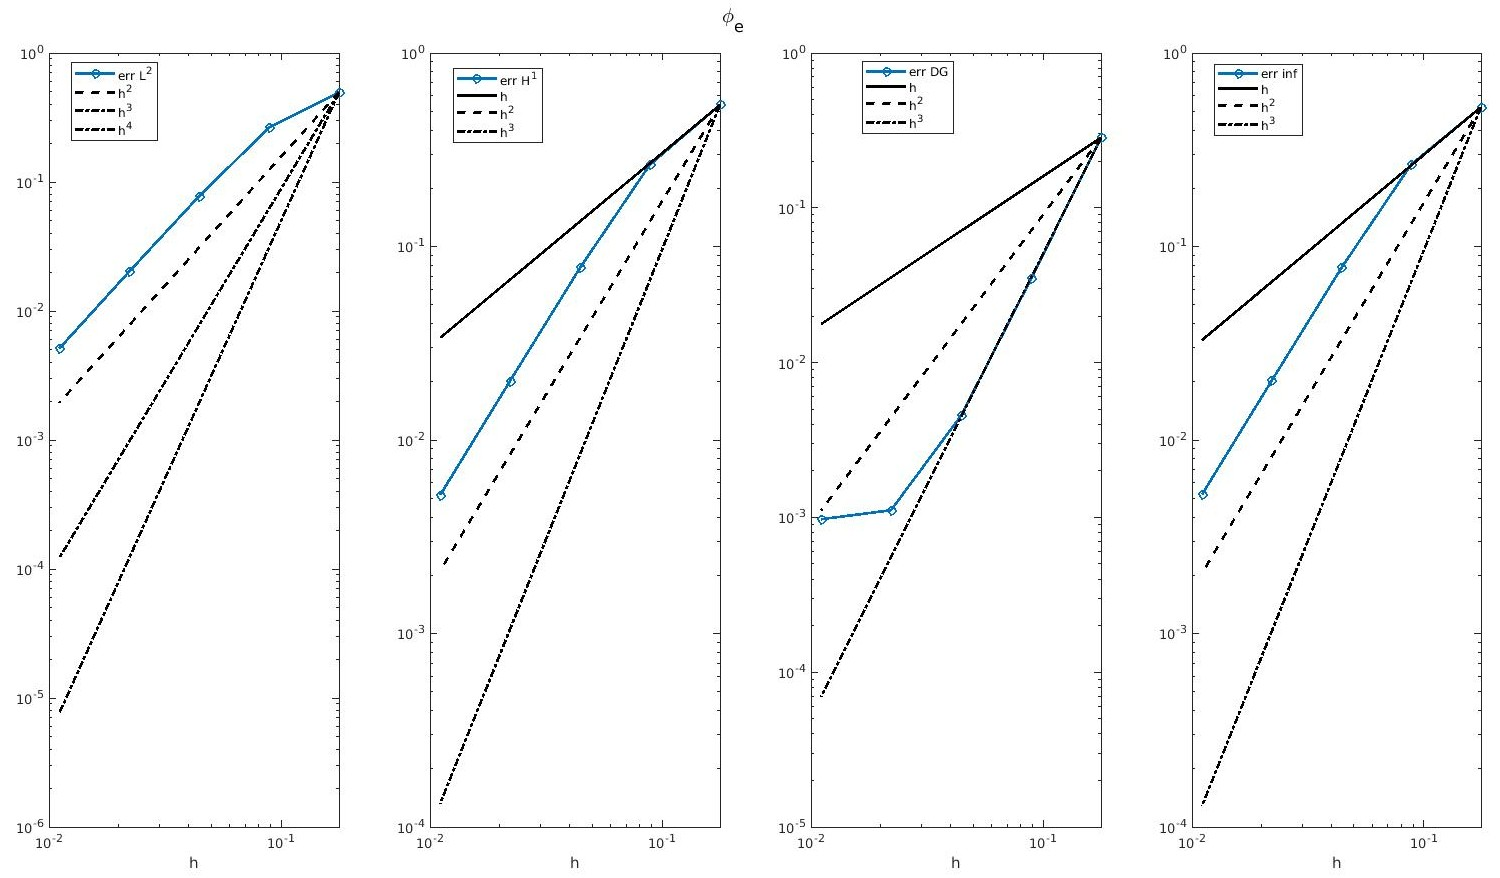
\includegraphics[width = 9cm]{./D3_Phie_1.jpg}
\caption{Extracellular Potential ($\phi_e$) with D3}
\end{subfigure}
\begin{subfigure}{0.5\textwidth}
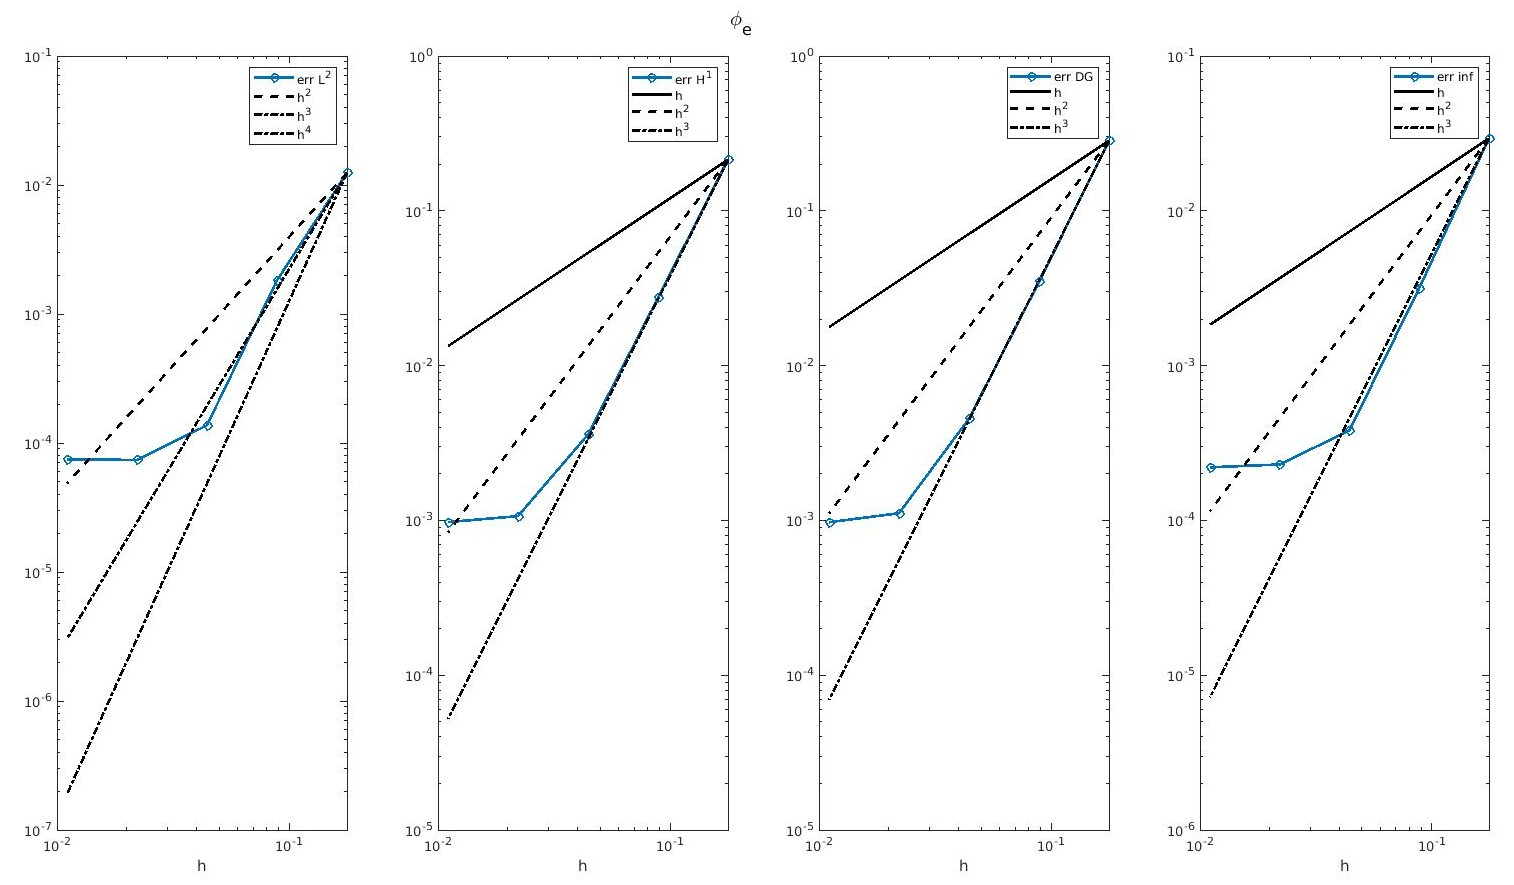
\includegraphics[width =9cm]{./P3_Phie_1.jpg}
\caption{Extracellular potential ($\phi_e$) with P3}
\label{Phie_P3}
\end{subfigure}
\begin{subfigure}{0.5\textwidth}
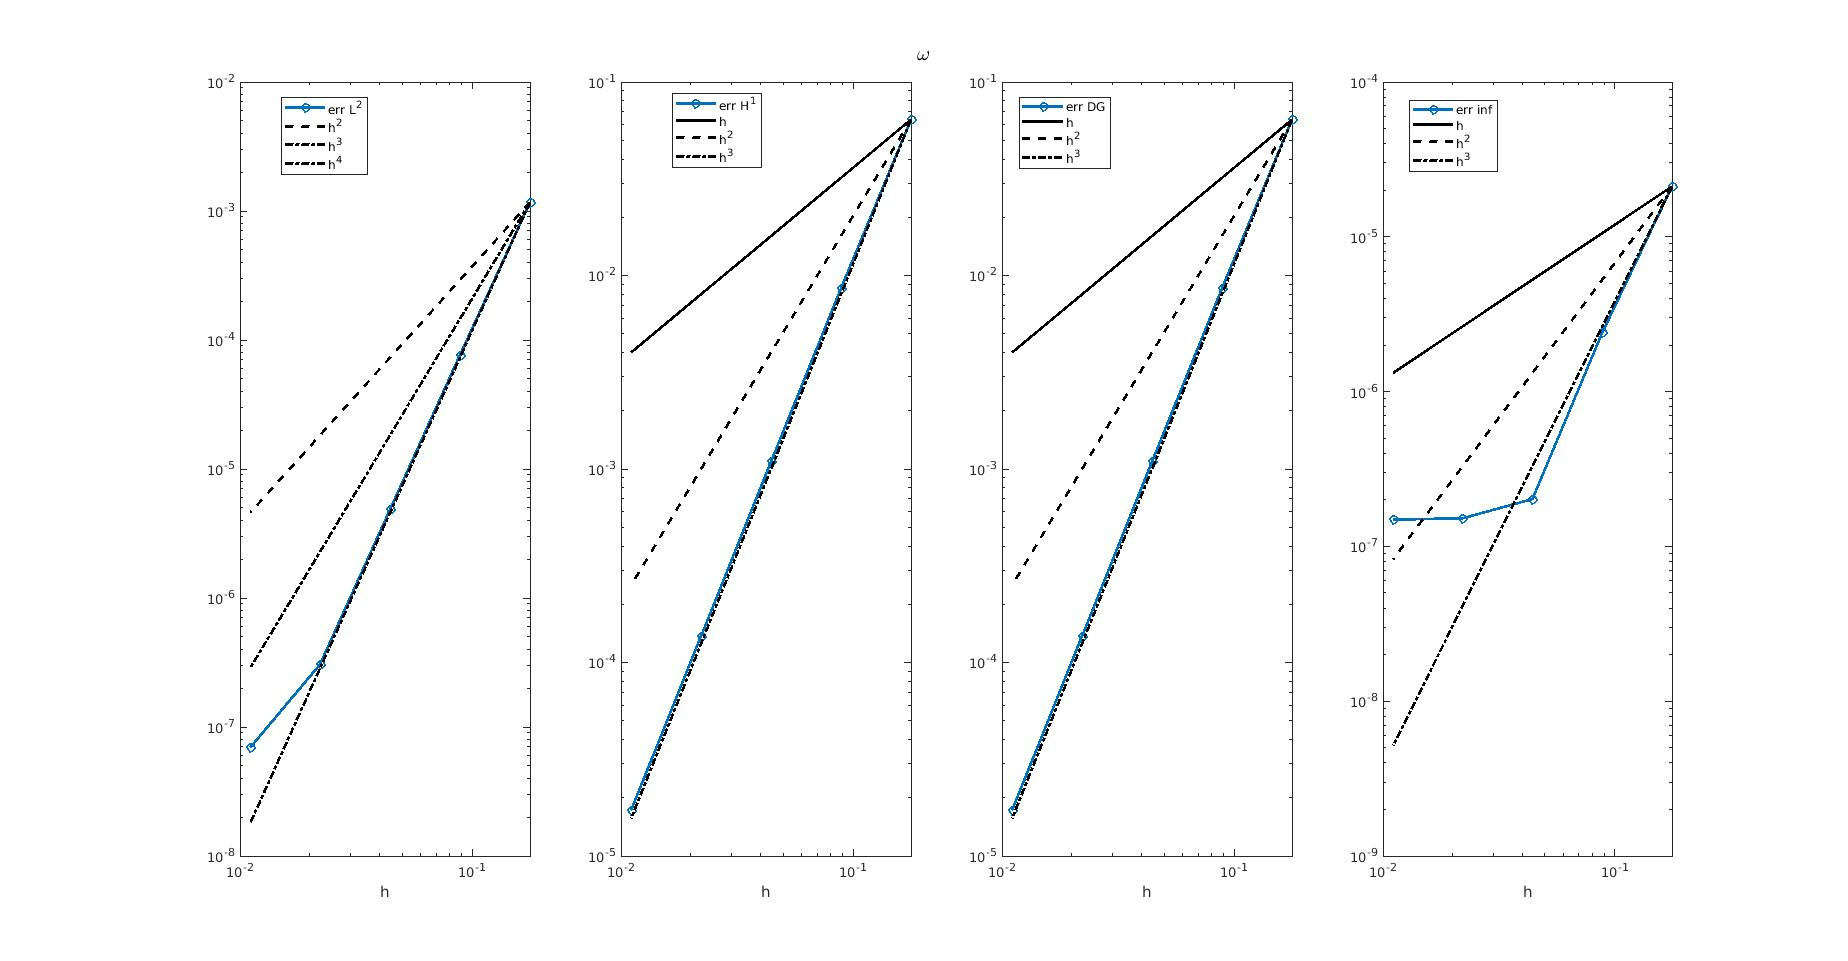
\includegraphics[width = 9cm]{./D3_w_1.jpg}
\caption{Gating variable ($w$) with D3}
\label{w_D3}
\end{subfigure}
\begin{subfigure}{0.5\textwidth}
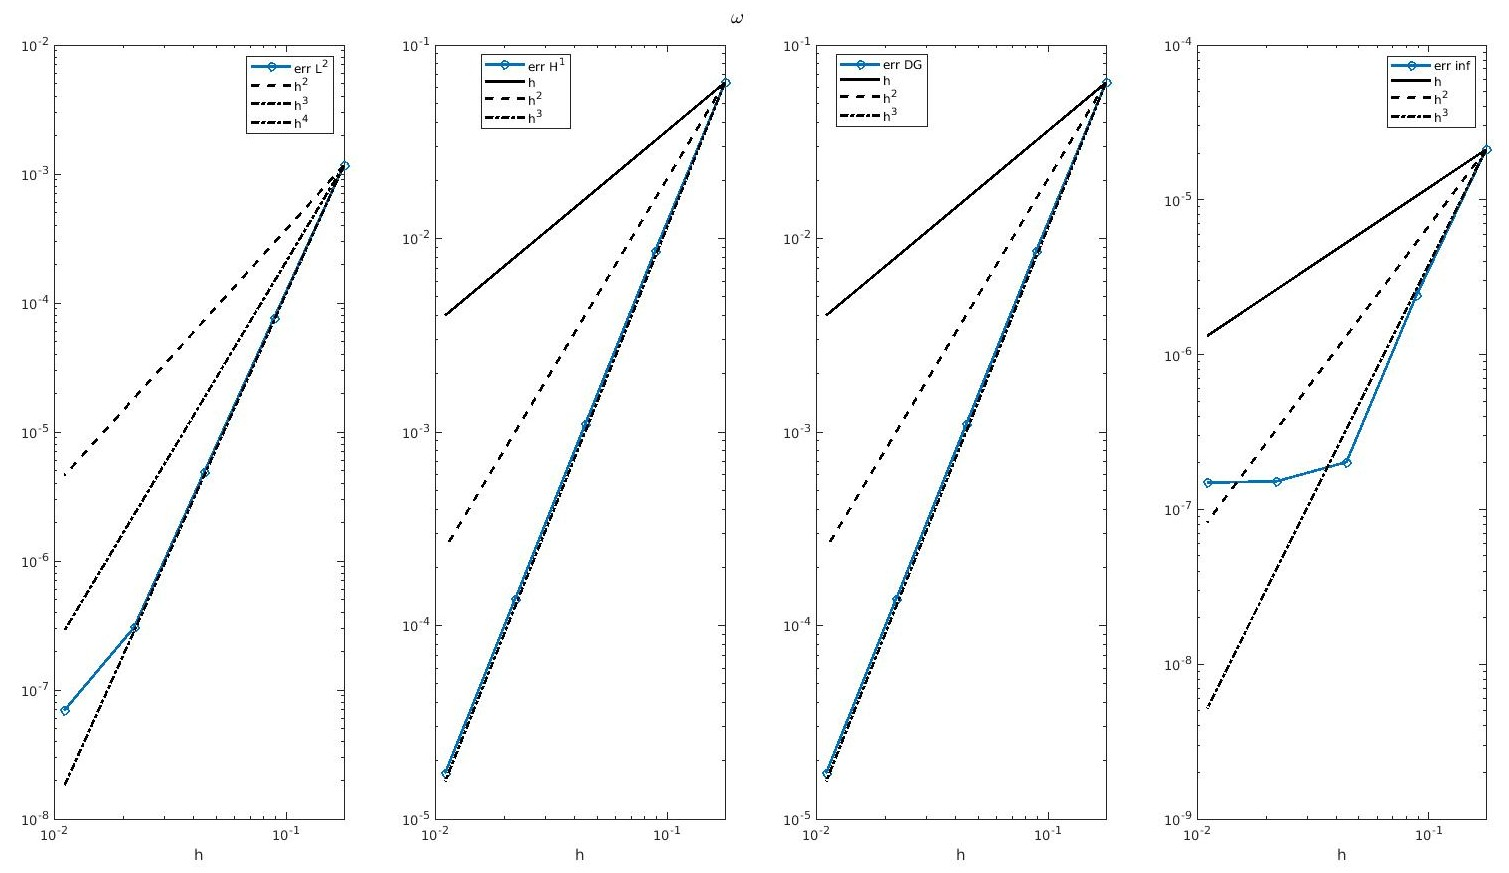
\includegraphics[width =9cm]{./P3_w_1.jpg}
\caption{Gating variable ($w$) with P3}
\label{w_P3}
\end{subfigure}
\end{figure}
\restoregeometry
\newpage
\subsection{Comparison between different time discretization methods}
In Section (\ref{temporal_discretization}) three methods for the time discretization have been proposed and discussed. An error analysis comparison has been executed and gives the graphical results shown in Fig. (\ref{Vm-time}) and Fig. (\ref{pe-time}). \\
\noindent It is clear that the three methods share an identical error trend. This is expected since they were initially defined with the same order. The main difference between the three is the explicit/implicit choice for the different terms that, in general, gives different results only in terms of stability and not of order. Moreover, it is noteworthy to remember that non-linear term is considered as explicit for all the methods and then no temporal strategy is completely implicit. For this reason, it may be that the three methods have very similar behavior under the stability aspect too.
\subsection{Comparison between methods for uniqueness of $\phi_i$ and $\phi_e$}
Referring to the Section (\ref{unique}), we have presented and explained two different methods to impose uniqueness of the cellular potentials.
The simplest one, adopted for the previous error analysis, imposes the value of the function in a specific point. On the other hand, the second imposes the mean value at zero. The comparison is displayed in Fig. (\ref{uniqueness_plot}). \\
\noindent First of all, we notice that the behavior for $V_m$ and $w$ are the same. This fact follows the theory since the imposition method affects only the values of the two potentials. On the other hand, for what concerns $\phi_i$ and $\phi_e$, we see very similar results (even if not identical, the second method seems slightly more regular in the $L^2$ norm). Indeed, as already anticipated in Section (\ref{uniqueness_results}), problems that does not imply very ill-conditioned systems can be solved in both ways with very small differences. Our proposed test-case belongs to this family and for this reason we adopted the first method for all the previous error analysis studies as it is almost equivalent to the second one. These plots, then, confirm that the two methods are consistent and, most of the times, equivalent. \\ \\
On the other hand, it has already been stated that some peculiar problems can be solved only using the second method. Indeed, the first method may have an overshooting effect that unbalances the solution. These problems will be considered in Section (\ref{real_sim}) about physical simulations. However, since there is no known analytical solution for these problems, we cannot make now an error analysis like the previous one.\\ \\
\noindent In conclusion, we successfully imposed the potentials uniqueness directly into the system thanks to these two strategies. For what concerns our two initial objectives (Section (\ref{imposition_section})), we achieved both them since:
\begin{itemize}
	\item Error analysis studies demonstrate that $\phi_i$ and $\phi_e$ potentials converge to the exact potentials as $V_m$ and $w$ do. Moreover, plots show that all the error orders are clearly defined.
	\item Conditional numbers turn to be considerably decreased. Our measures proved that they passed from $\approx 10^{17}$ to $\approx 10^{7}$ for both the strategies.
\end{itemize}
\newpage
\newgeometry{a4paper,top=0.9cm,bottom=2cm,left=1cm,right=1cm} 
\begin{figure}[h]  \captionsetup{size = large} \caption{Comparison of $V_m$ and $\phi_i$ errors between different time-discretization schemes} \label{Vm-time}
\begin{subfigure}{0.5\textwidth}
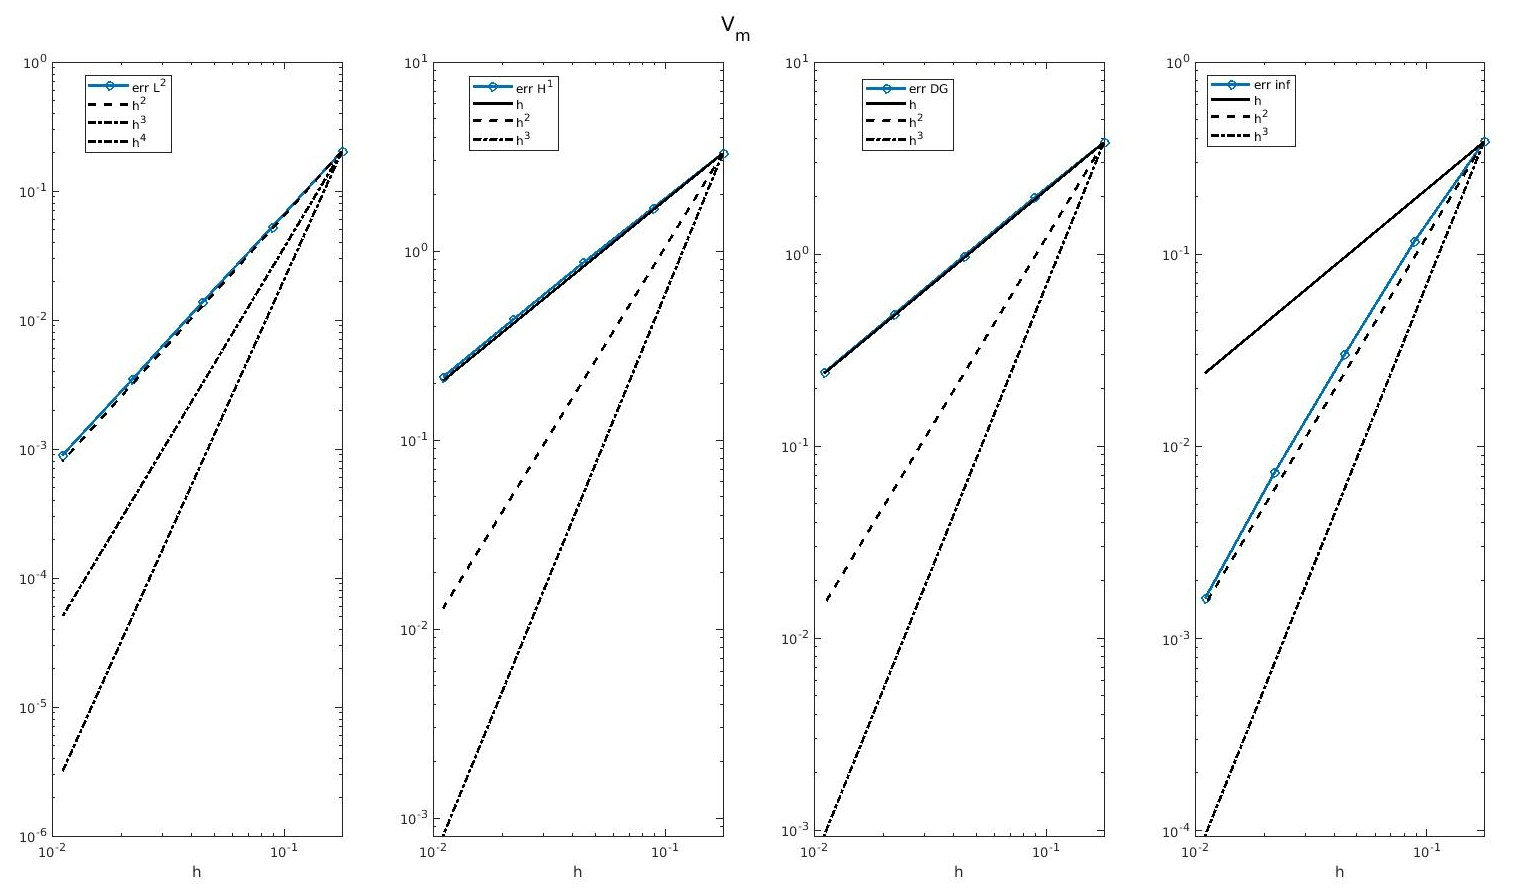
\includegraphics[width = 9cm]{./D1_Vm_1.jpg}
\caption*{$V_m$ with D1 - Semi-implicit method}
\end{subfigure}
\begin{subfigure}{0.5\textwidth}
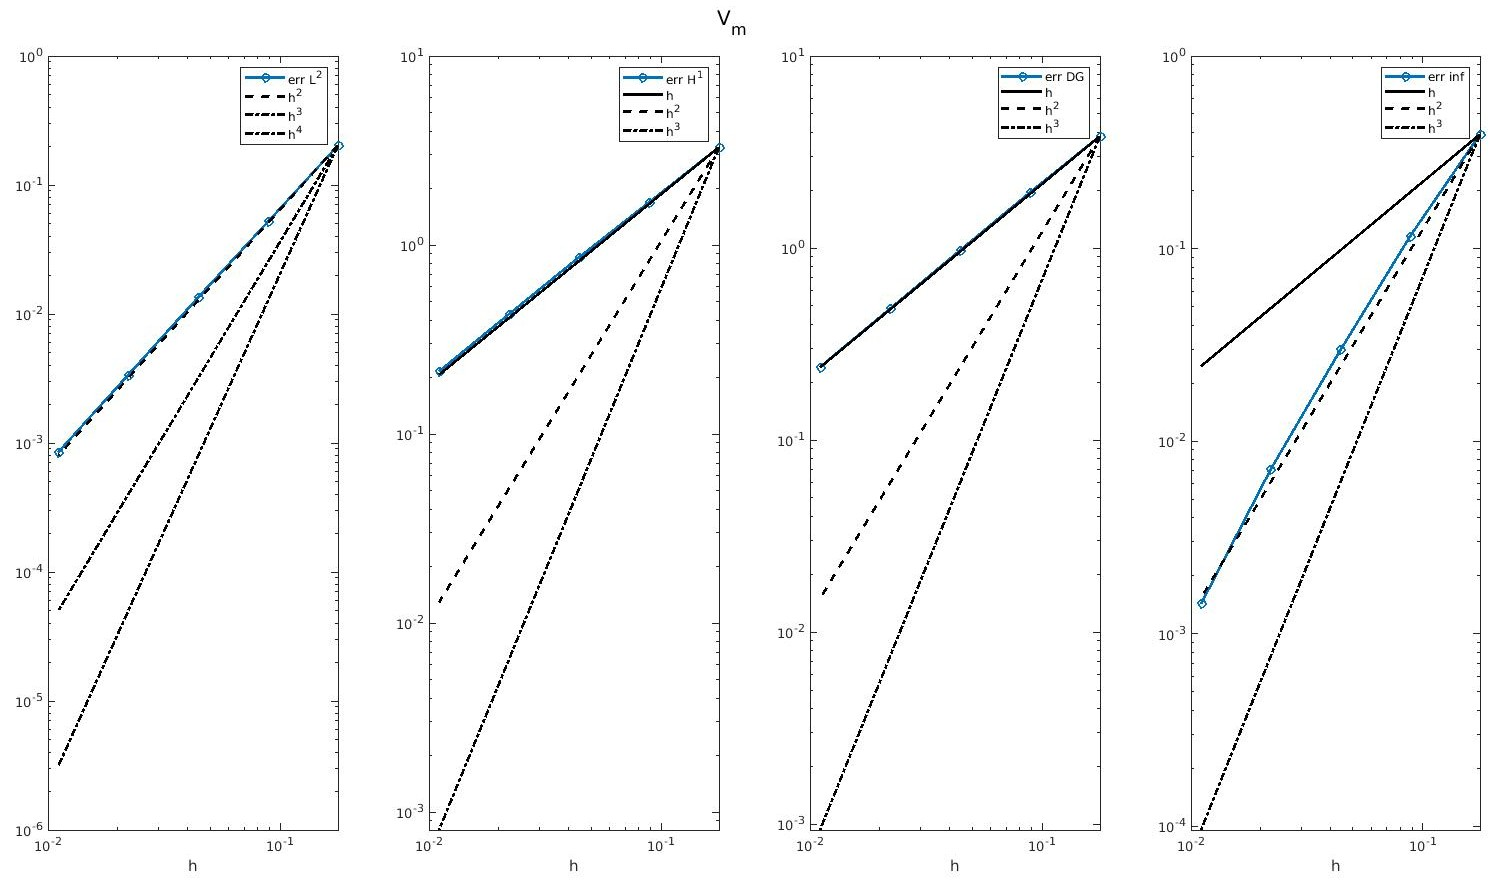
\includegraphics[width =9cm]{./D1_Vm_1_GO.jpg}
\caption*{$V_m$ with D1 - Godunov operator-splitting method}
\end{subfigure}
\begin{center}
\begin{subfigure}{0.5\textwidth}
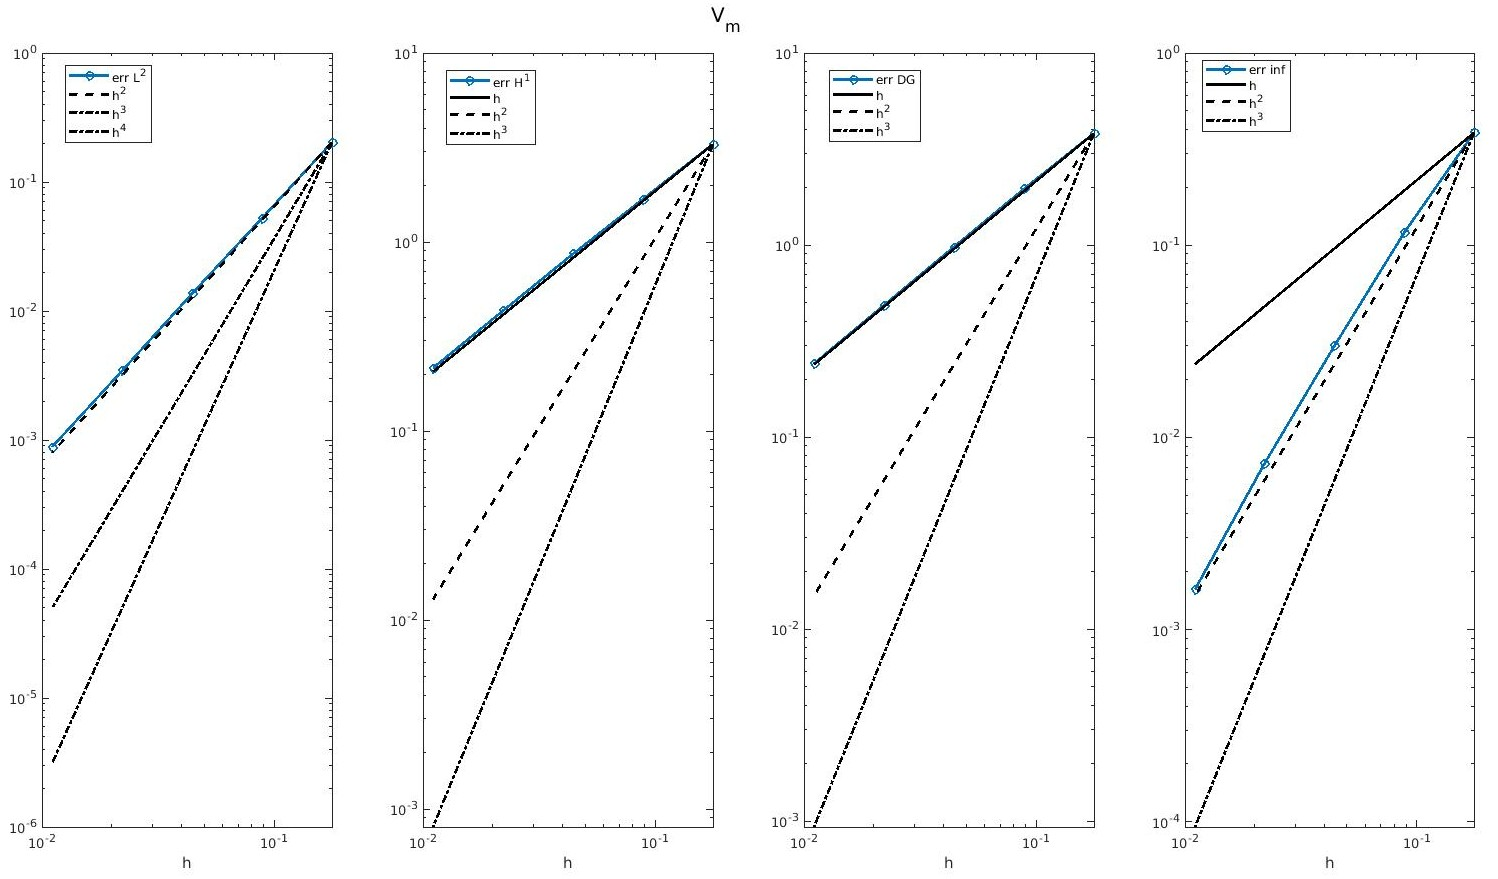
\includegraphics[width =9cm]{./D1_Vm_1_OS.jpg}
\caption*{$V_m$ with D1 - Quasi-implicit operator-splitting method}
\end{subfigure}
\end{center}
\begin{subfigure}{0.5\textwidth}
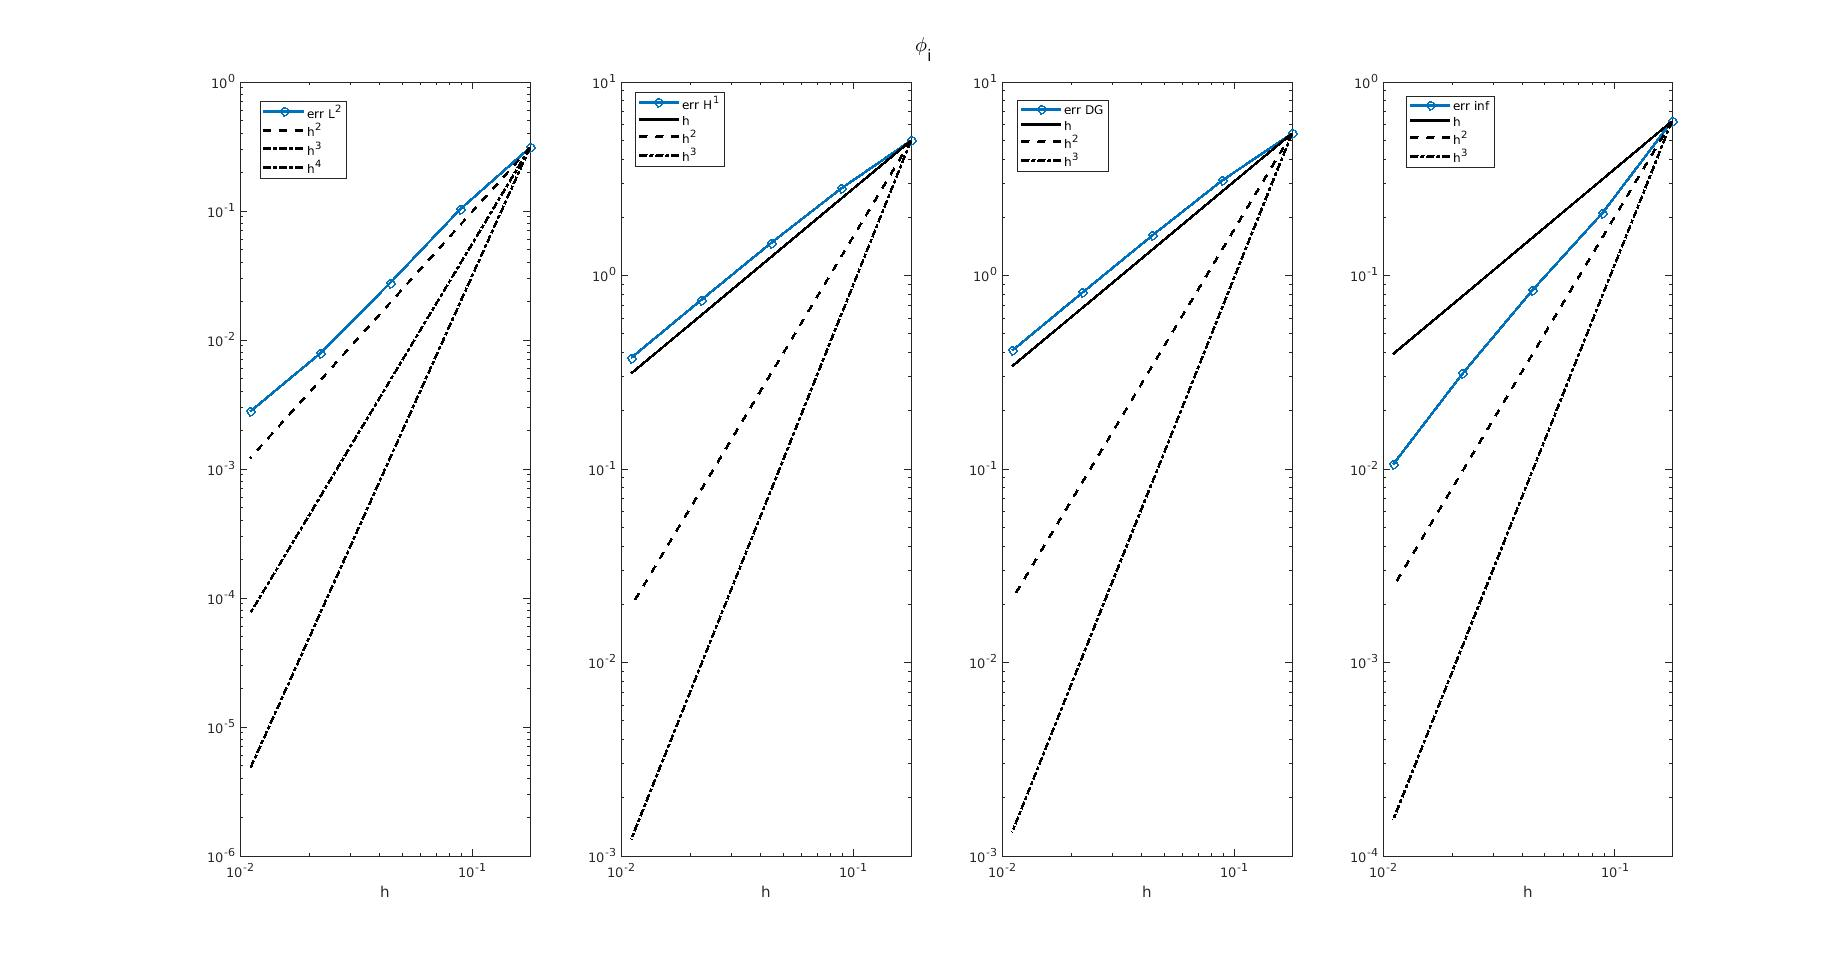
\includegraphics[width = 9cm]{./D1_Phii_1.jpg}
\caption*{$\phi_i$ with D1 - Semi-implicit method}
\end{subfigure}
\begin{subfigure}{0.5\textwidth}
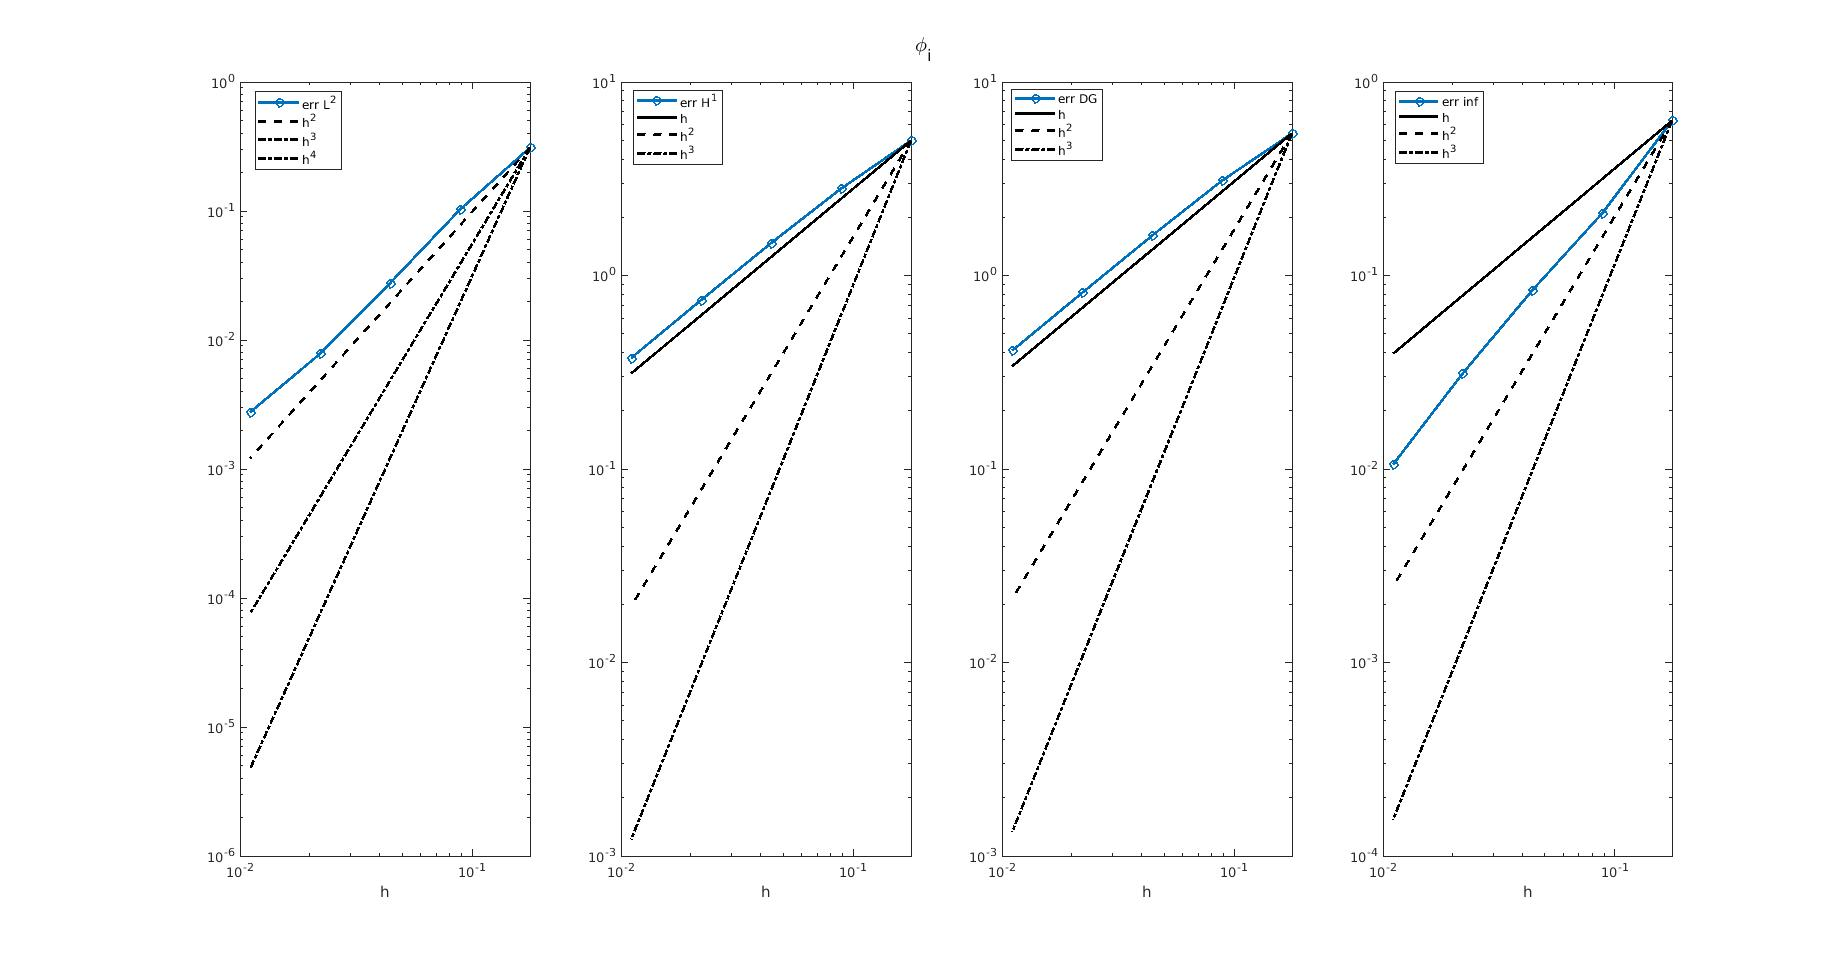
\includegraphics[width =9cm]{./D1_Phii_1_GO.jpg}
\caption*{$\phi_i$ with D1 - Godunov operator-splitting method}
\end{subfigure}
\begin{center}
\begin{subfigure}{0.5\textwidth}
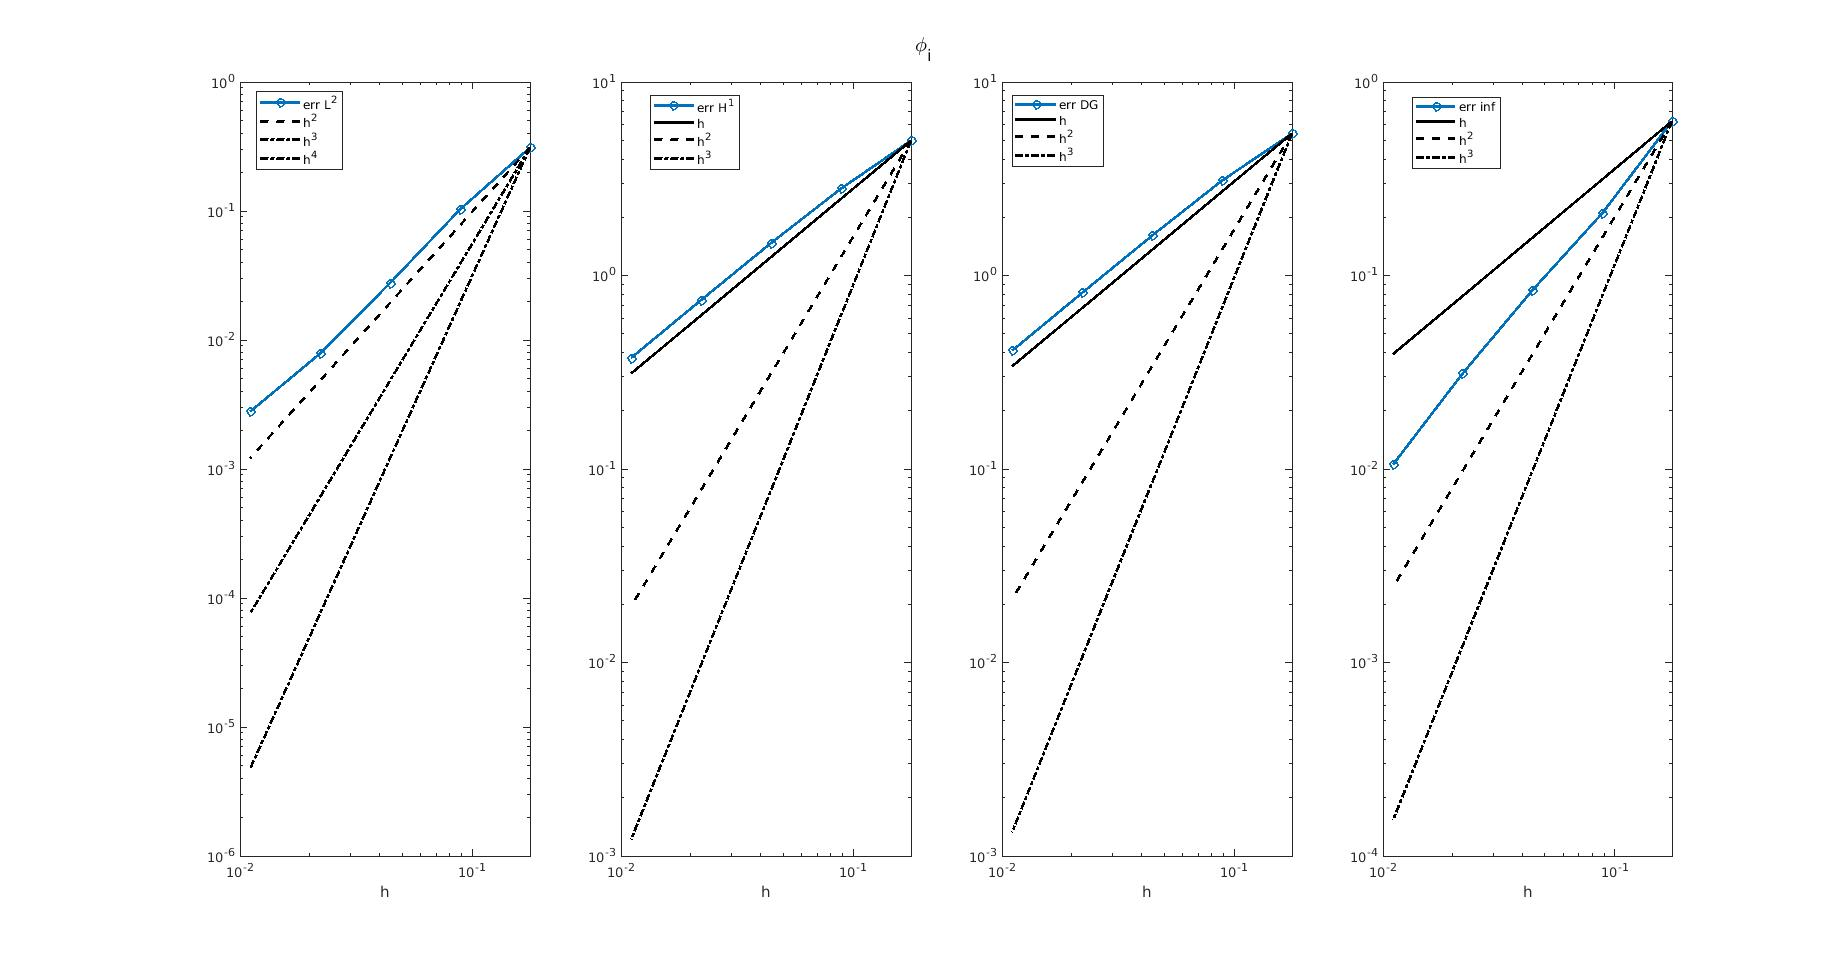
\includegraphics[width =9cm]{./D1_Phii_1_OS.jpg}
\caption*{$\phi_i$ with D1 - Quasi-implicit operator-splitting method}
\end{subfigure}
\end{center}
\end{figure}

\newpage

\begin{figure} \captionsetup{size = large} \caption{Comparison of $\phi_e$ and $w$ errors between different time-discretization schemes} \label{pe-time}
\begin{subfigure}{0.5\textwidth}
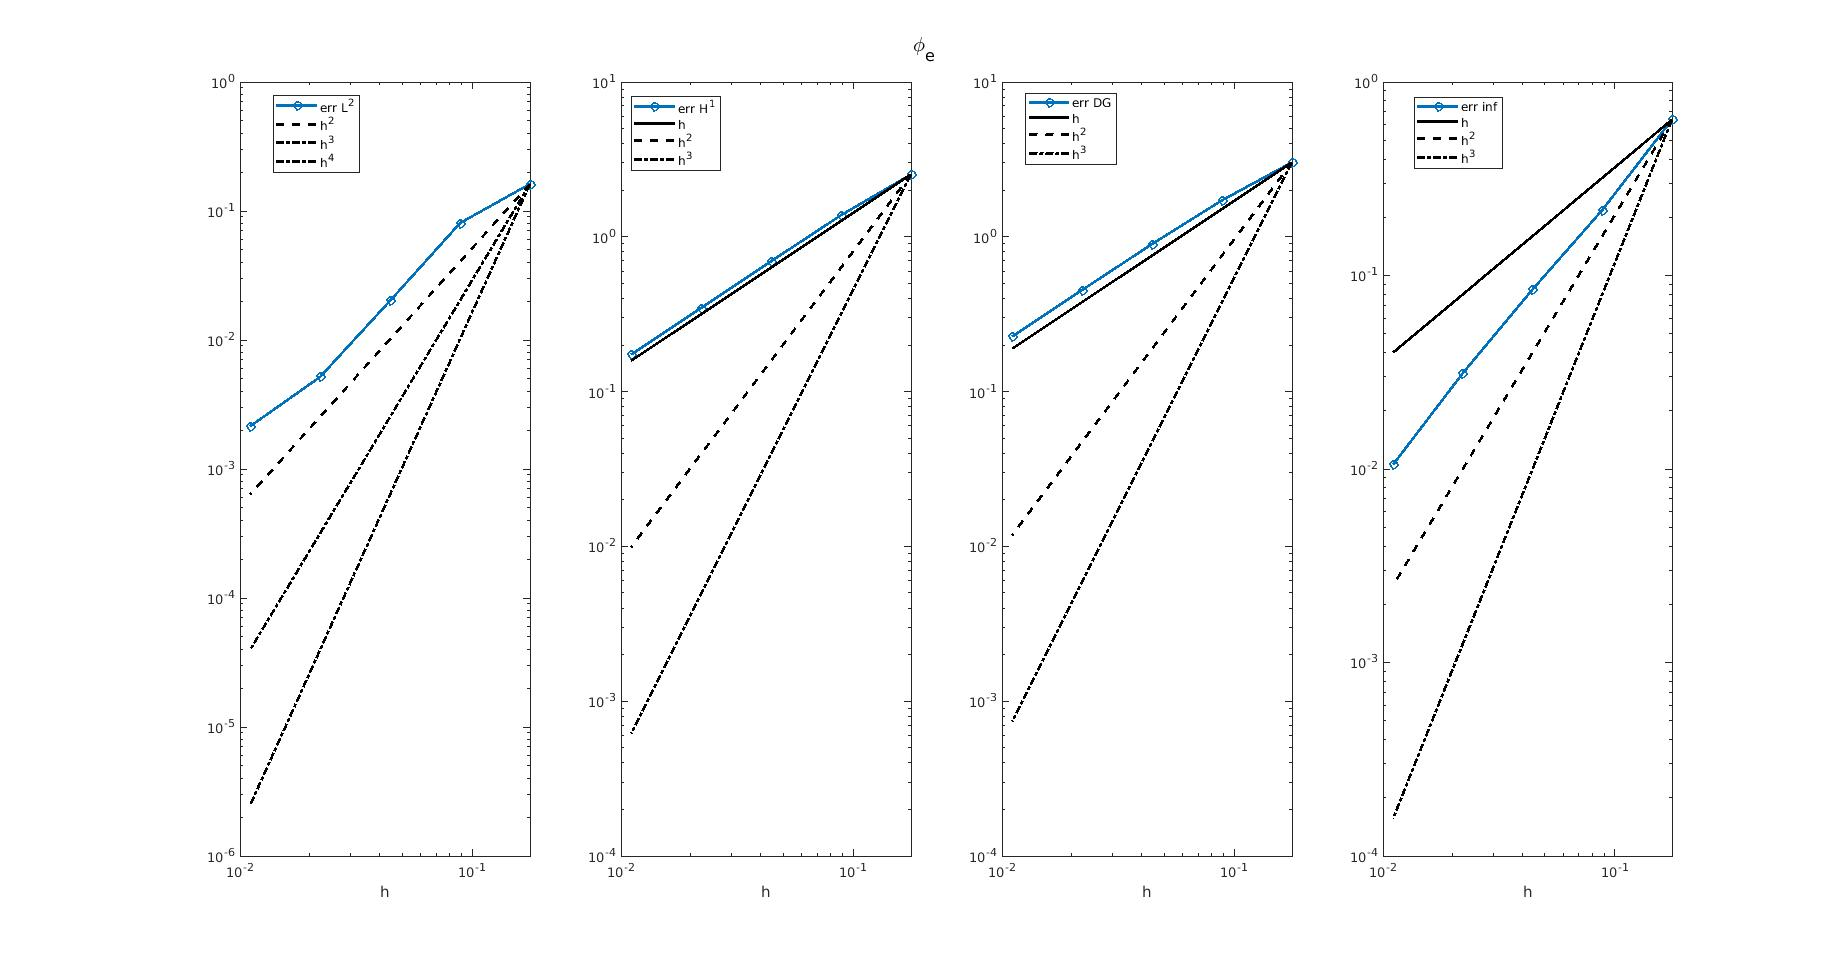
\includegraphics[width = 9cm]{./D1_Phie_1.jpg}
\caption*{$\phi_e$ with D1 - Semi-implicit method}
\end{subfigure}
\begin{subfigure}{0.5\textwidth}
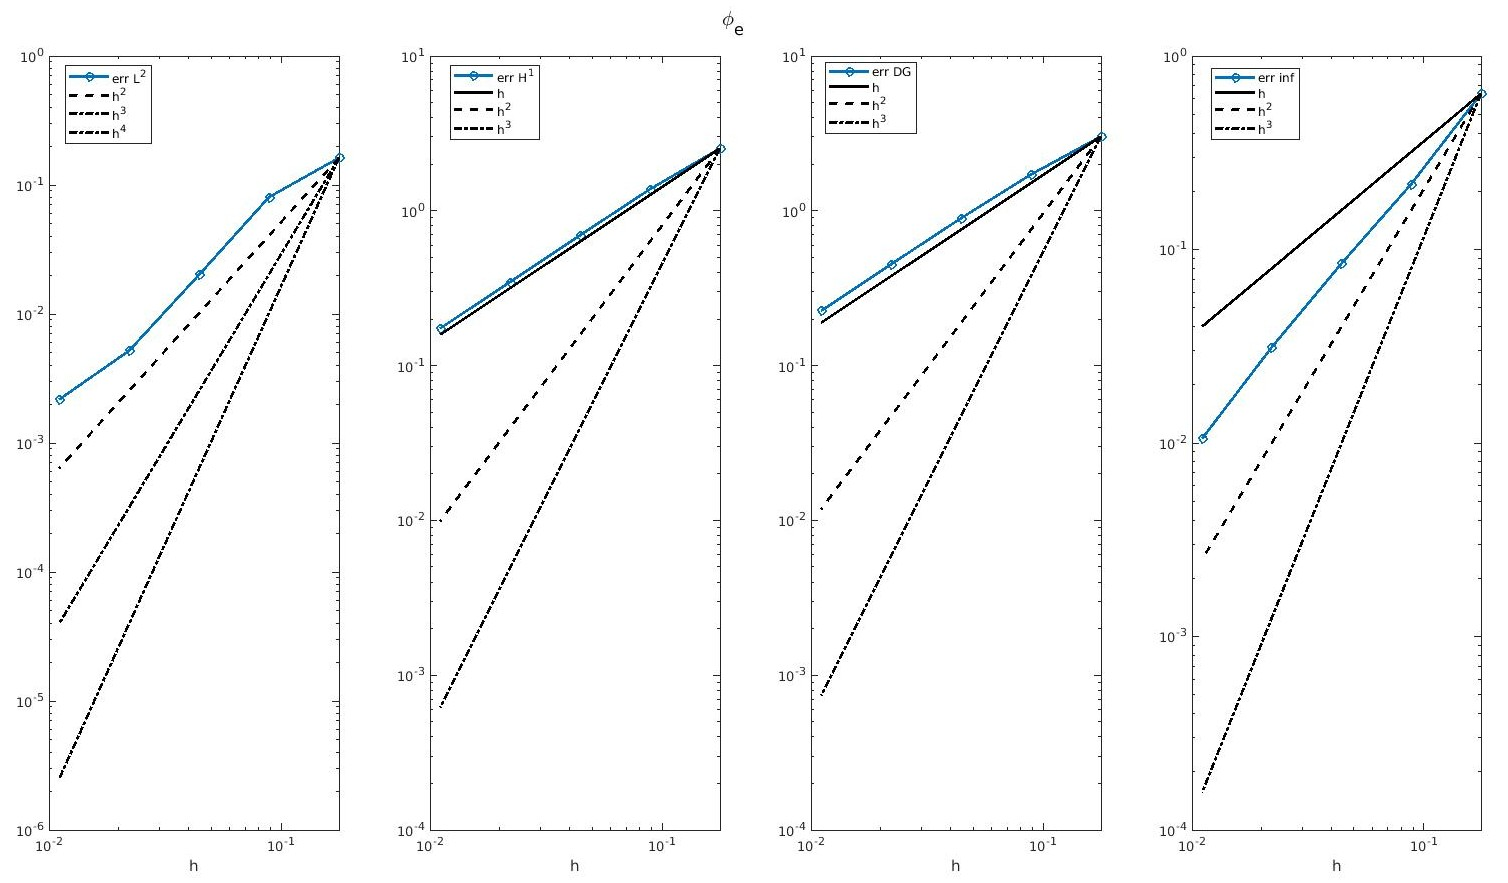
\includegraphics[width =9cm]{./D1_Phie_1_GO.jpg}
\caption*{$\phi_e$ with D1 - Godunov operator-splitting method}
\end{subfigure}
\begin{center}
\begin{subfigure}{0.5\textwidth}
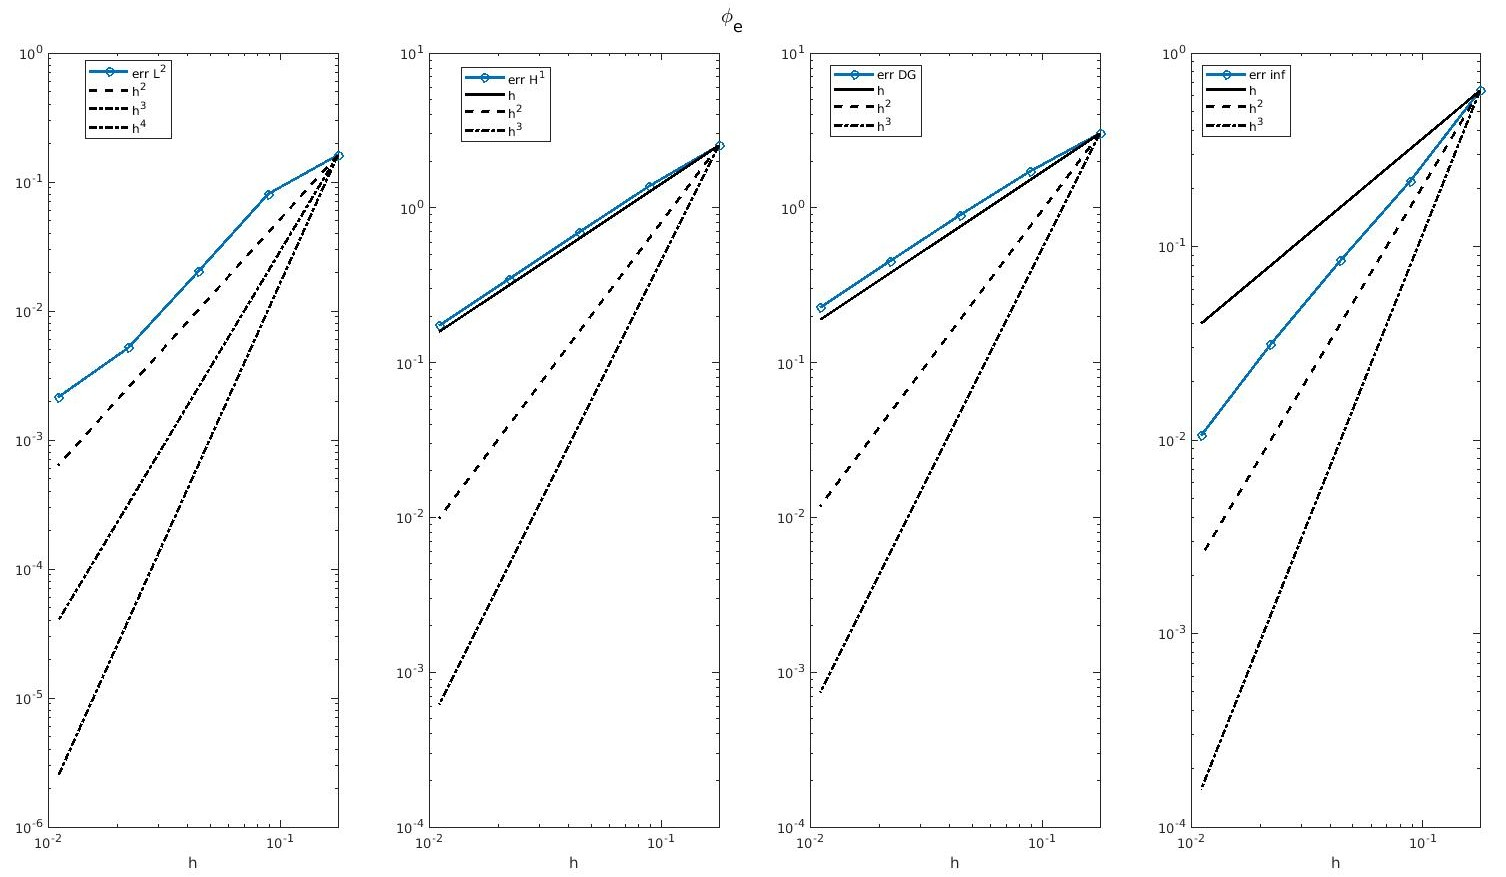
\includegraphics[width =9cm]{./D1_Phie_1_OS.jpg}
\caption*{$\phi_e$ with D1 - Quasi-implicit operator-splitting method}
\end{subfigure}
\end{center}
\begin{subfigure}{0.5\textwidth}
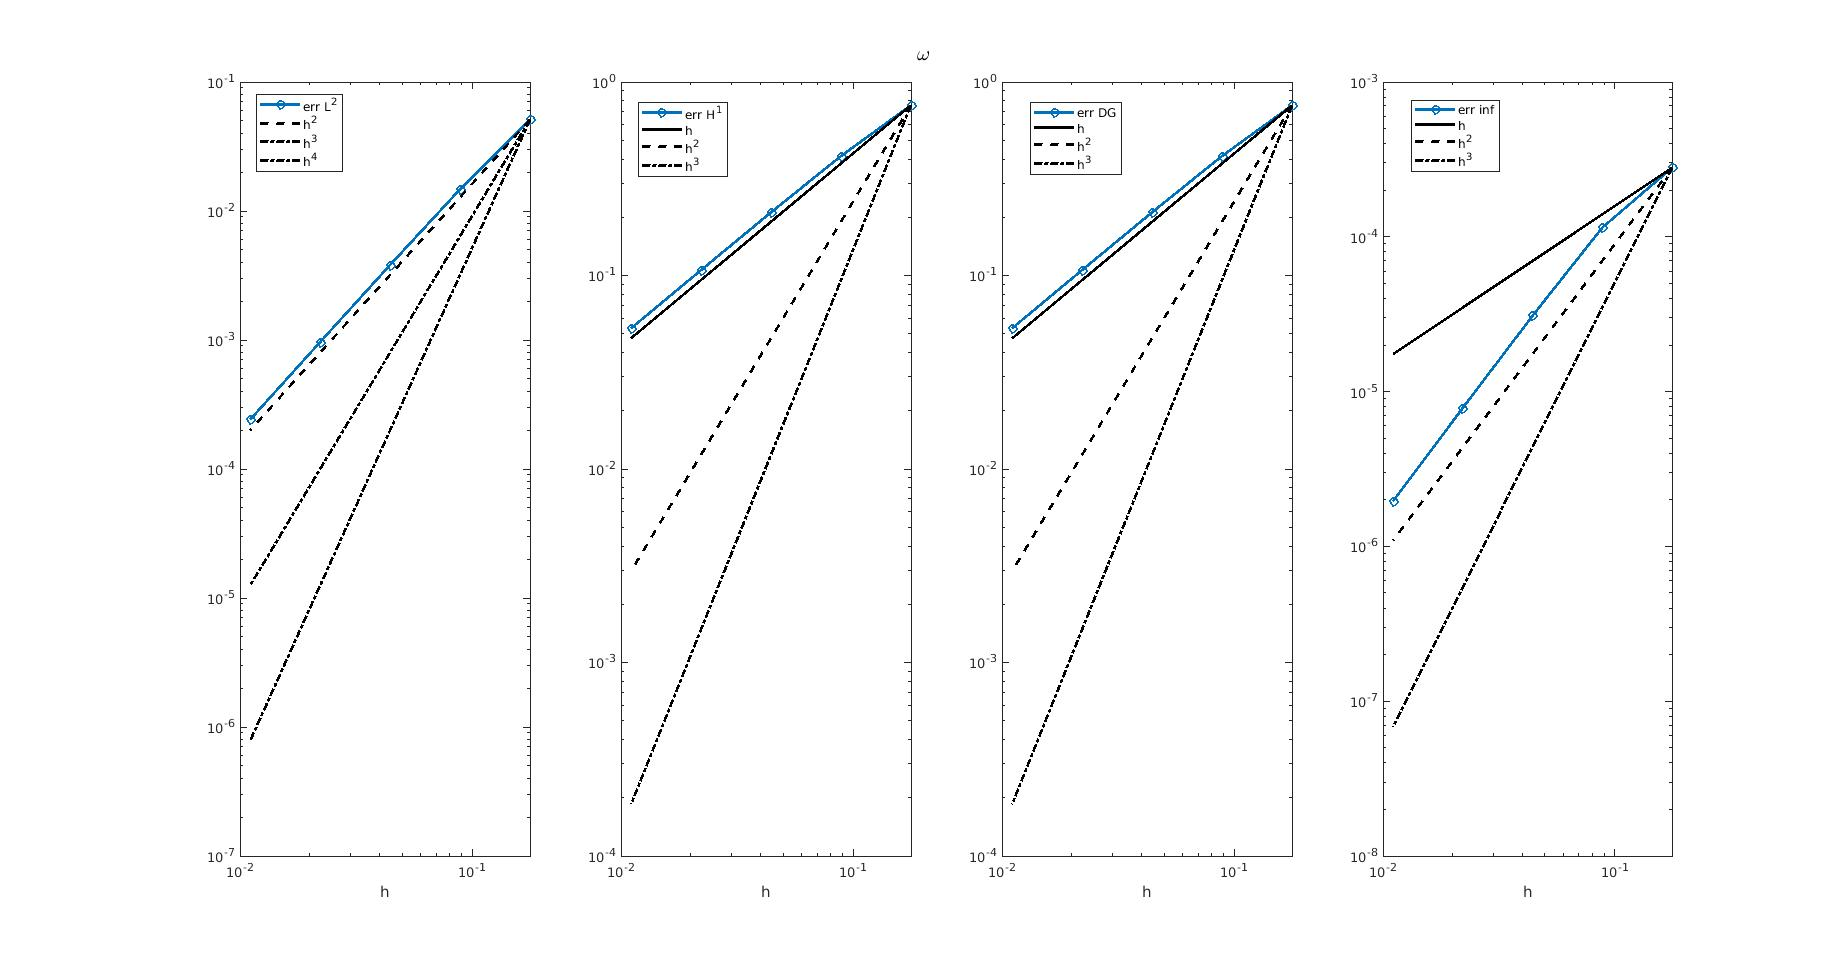
\includegraphics[width = 9cm]{./D1_w_1.jpg}
\caption*{$w$ with D1 - Semi-implicit method}
\end{subfigure}
\begin{subfigure}{0.5\textwidth}
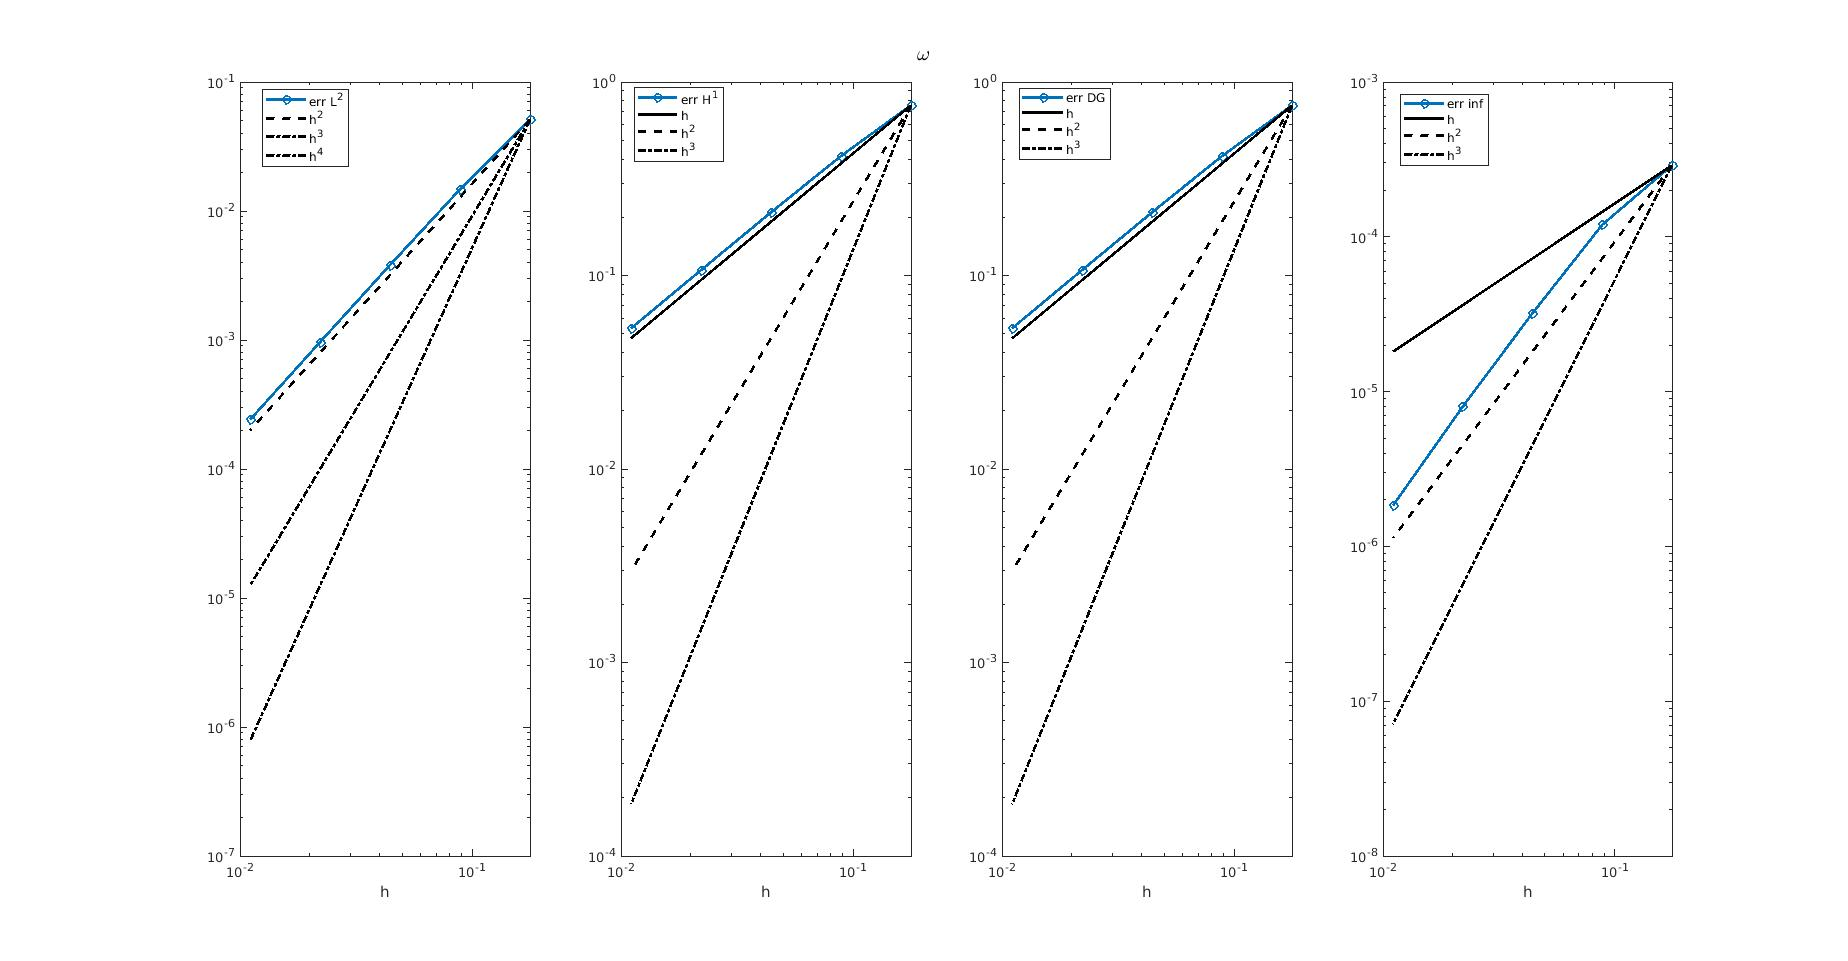
\includegraphics[width =9cm]{./D1_w_1_GO.jpg}
\caption*{$w$ with D1 - Godunov operator-splitting method}
\end{subfigure}
\begin{center}
\begin{subfigure}{0.5\textwidth}
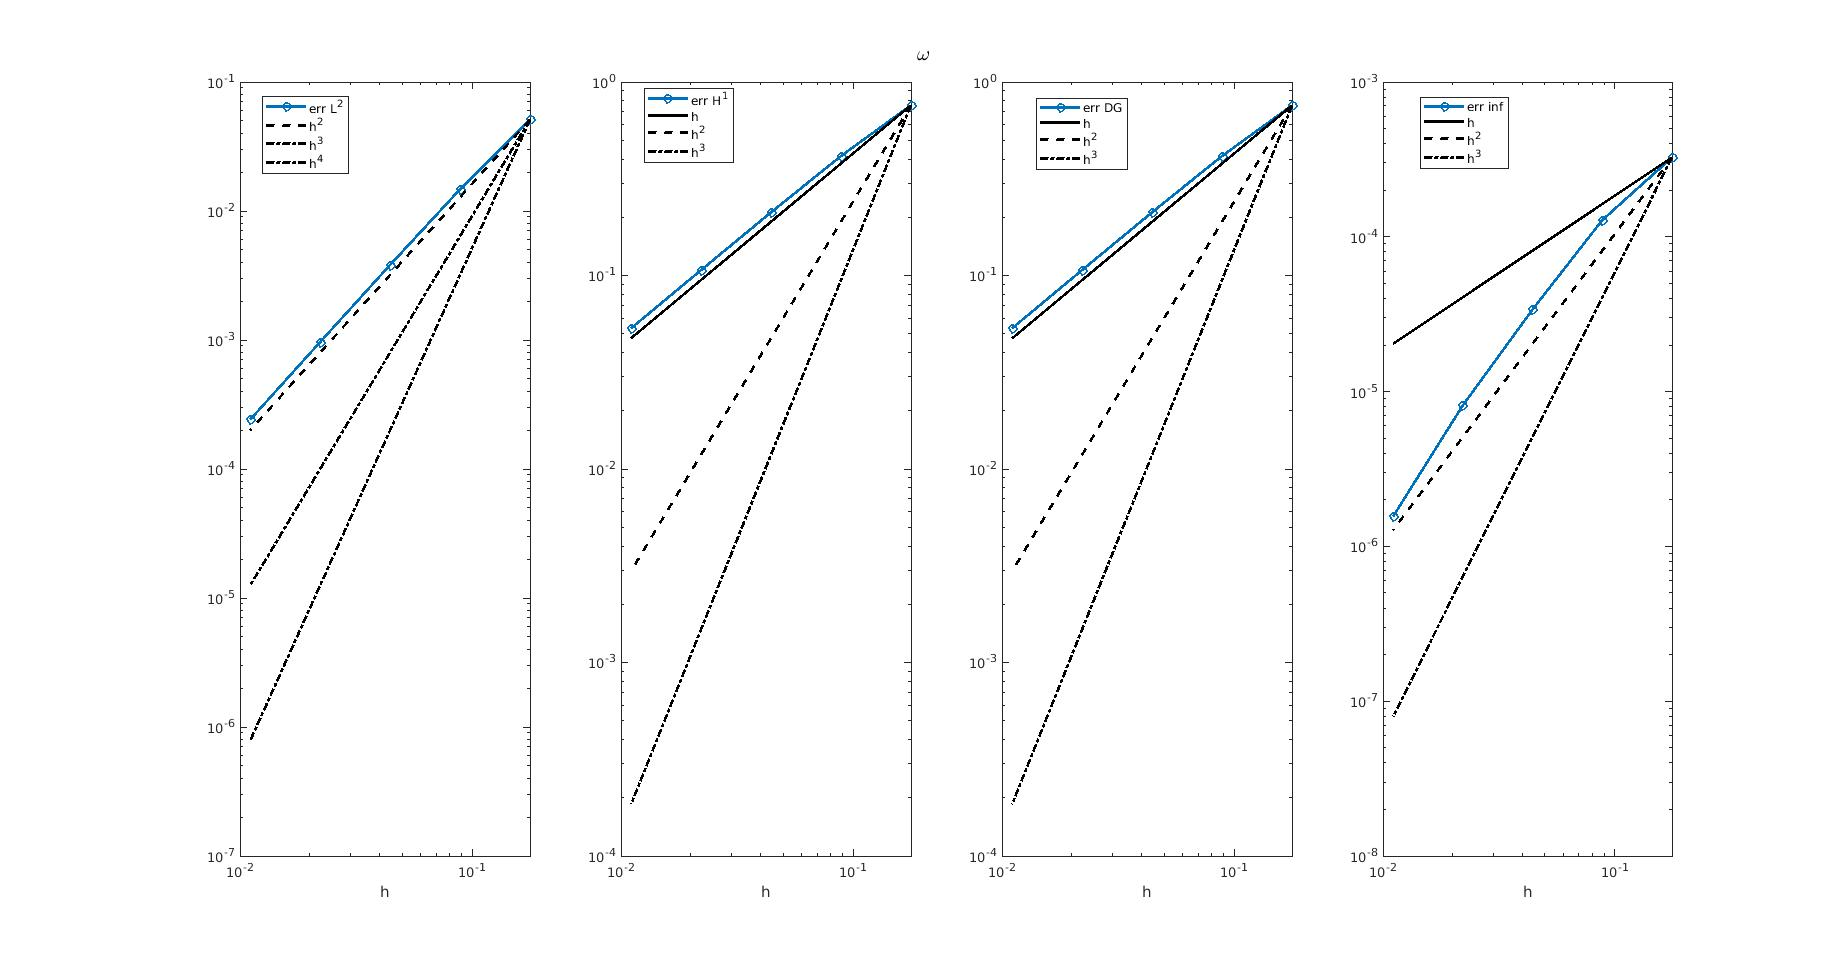
\includegraphics[width =9cm]{./D1_w_1_OS.jpg}
\caption*{$w$ with D1 - Quasi-implicit operator-splitting method}
\end{subfigure}
\end{center}
\end{figure}
\restoregeometry
\newpage

\newgeometry{a4paper,top=1cm,bottom=2cm,left=1cm,right=1cm} 
\begin{figure}[h] \captionsetup{size = large} \caption{Comparison between the uniqueness imposition strategies} \label{uniqueness_plot}
\begin{subfigure}{0.5\textwidth}
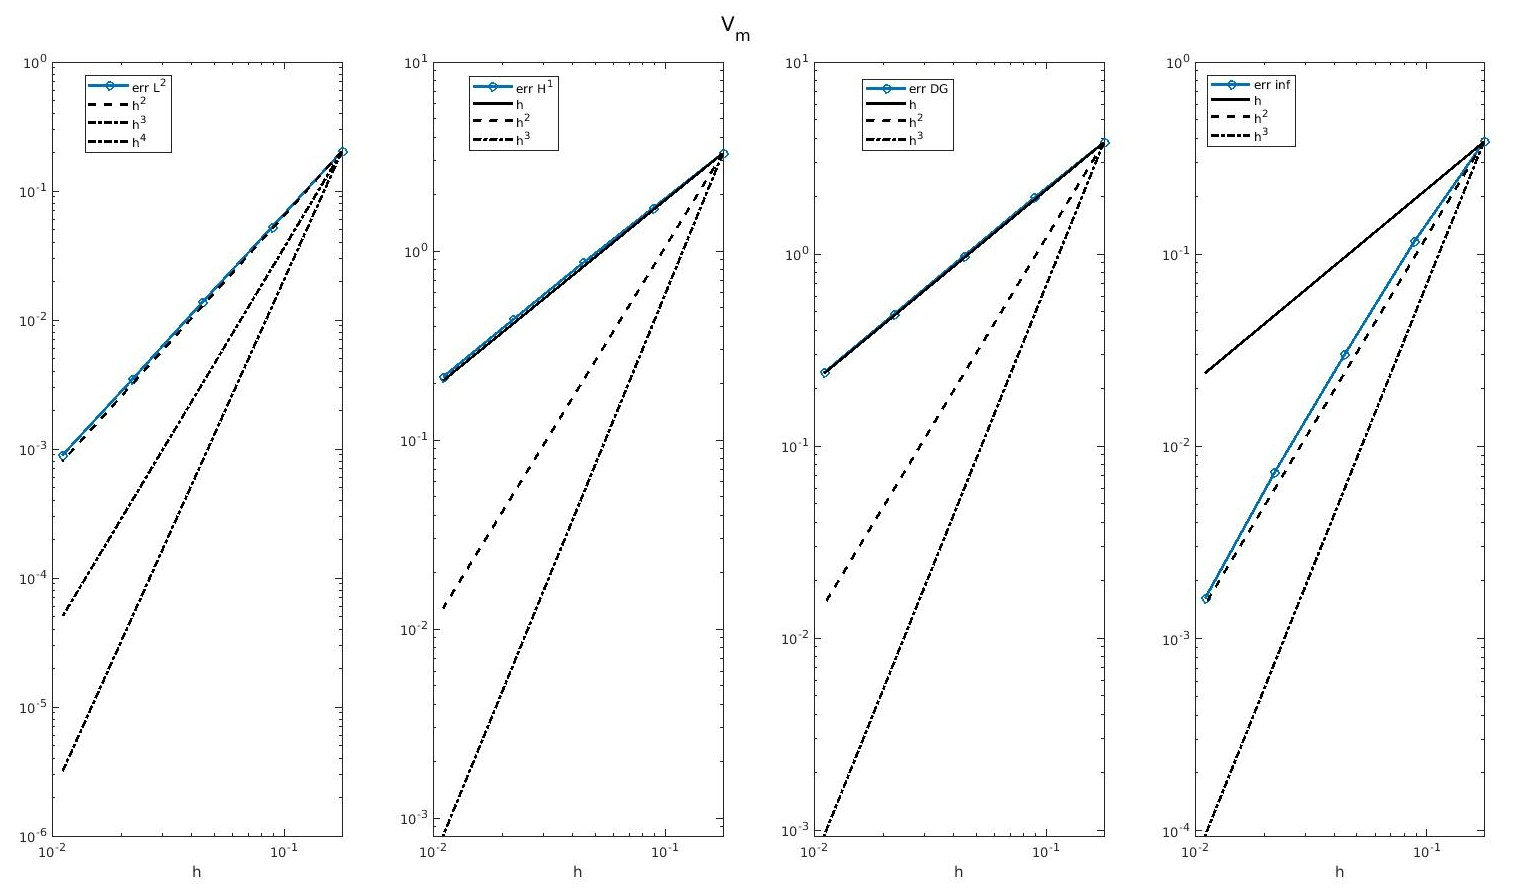
\includegraphics[width = 9cm]{./D1_Vm_1.jpg}
\caption*{$V_m$ with D1 imposing the function in a specific point}
\label{Vm_1}
\end{subfigure}
\begin{subfigure}{0.5\textwidth}
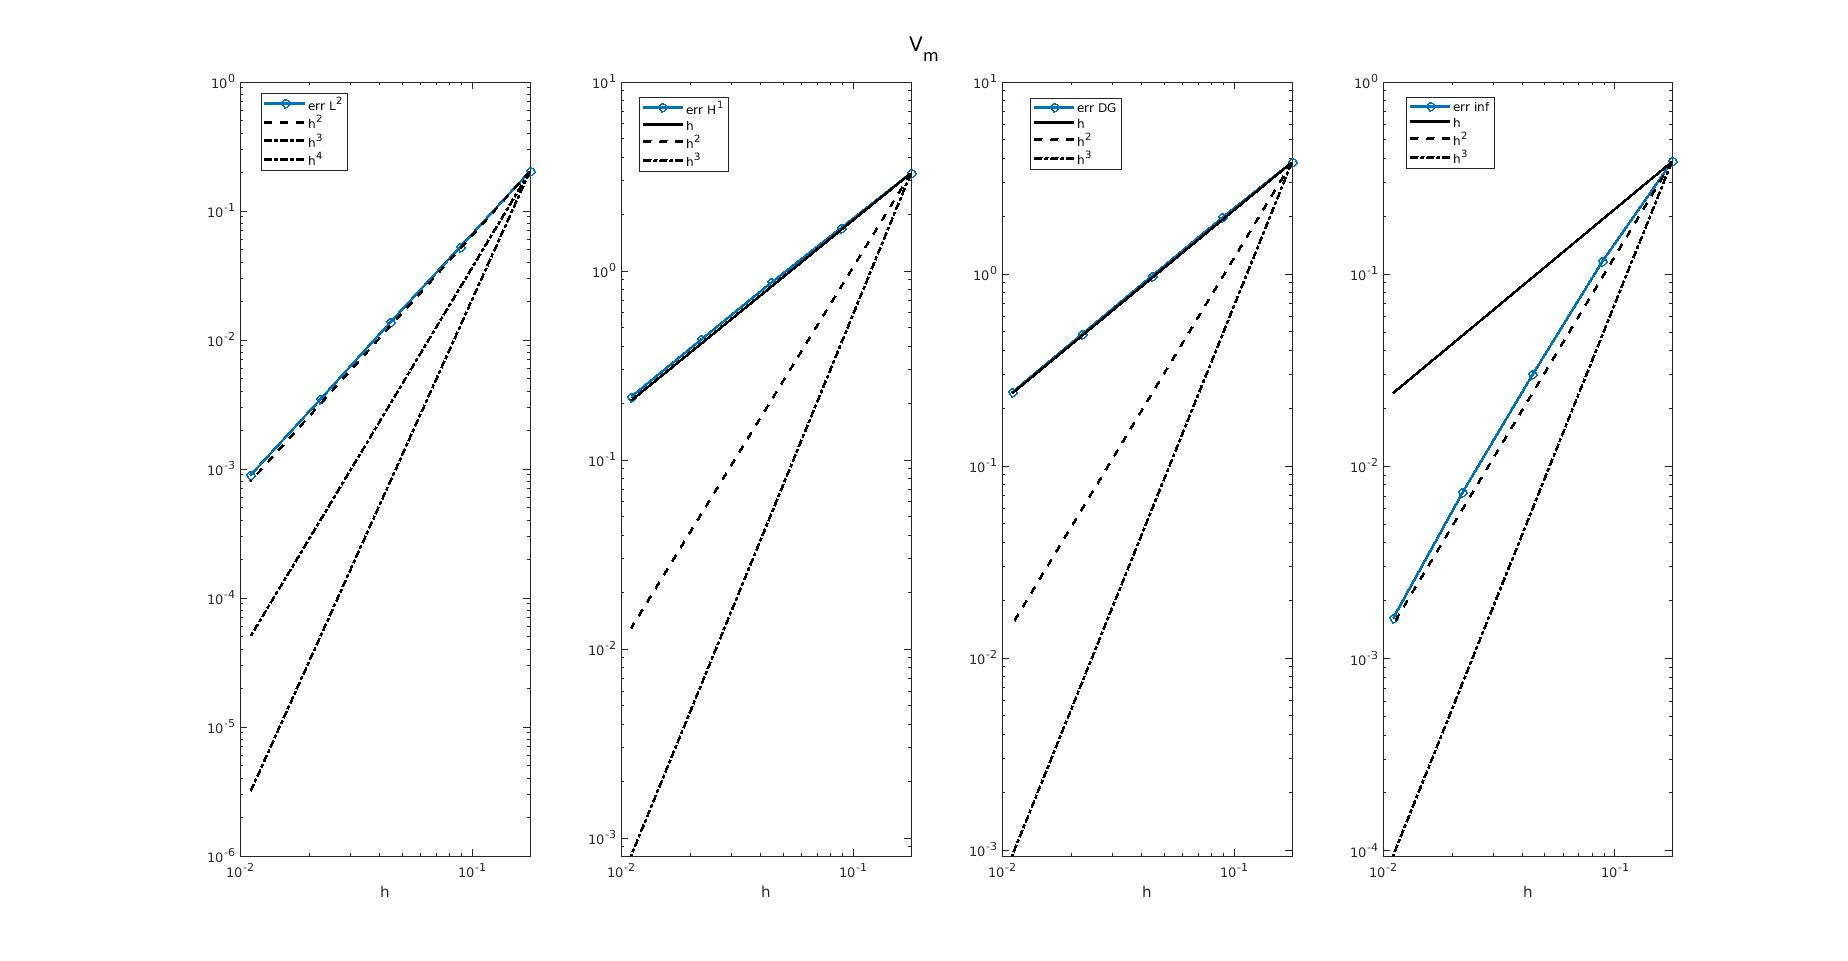
\includegraphics[width =9cm]{./D1_Vm_2.jpg}
\caption*{$V_m$ with D1 imposing the zero mean}
\label{Vm_2}
\end{subfigure}
\begin{subfigure}{0.5\textwidth}
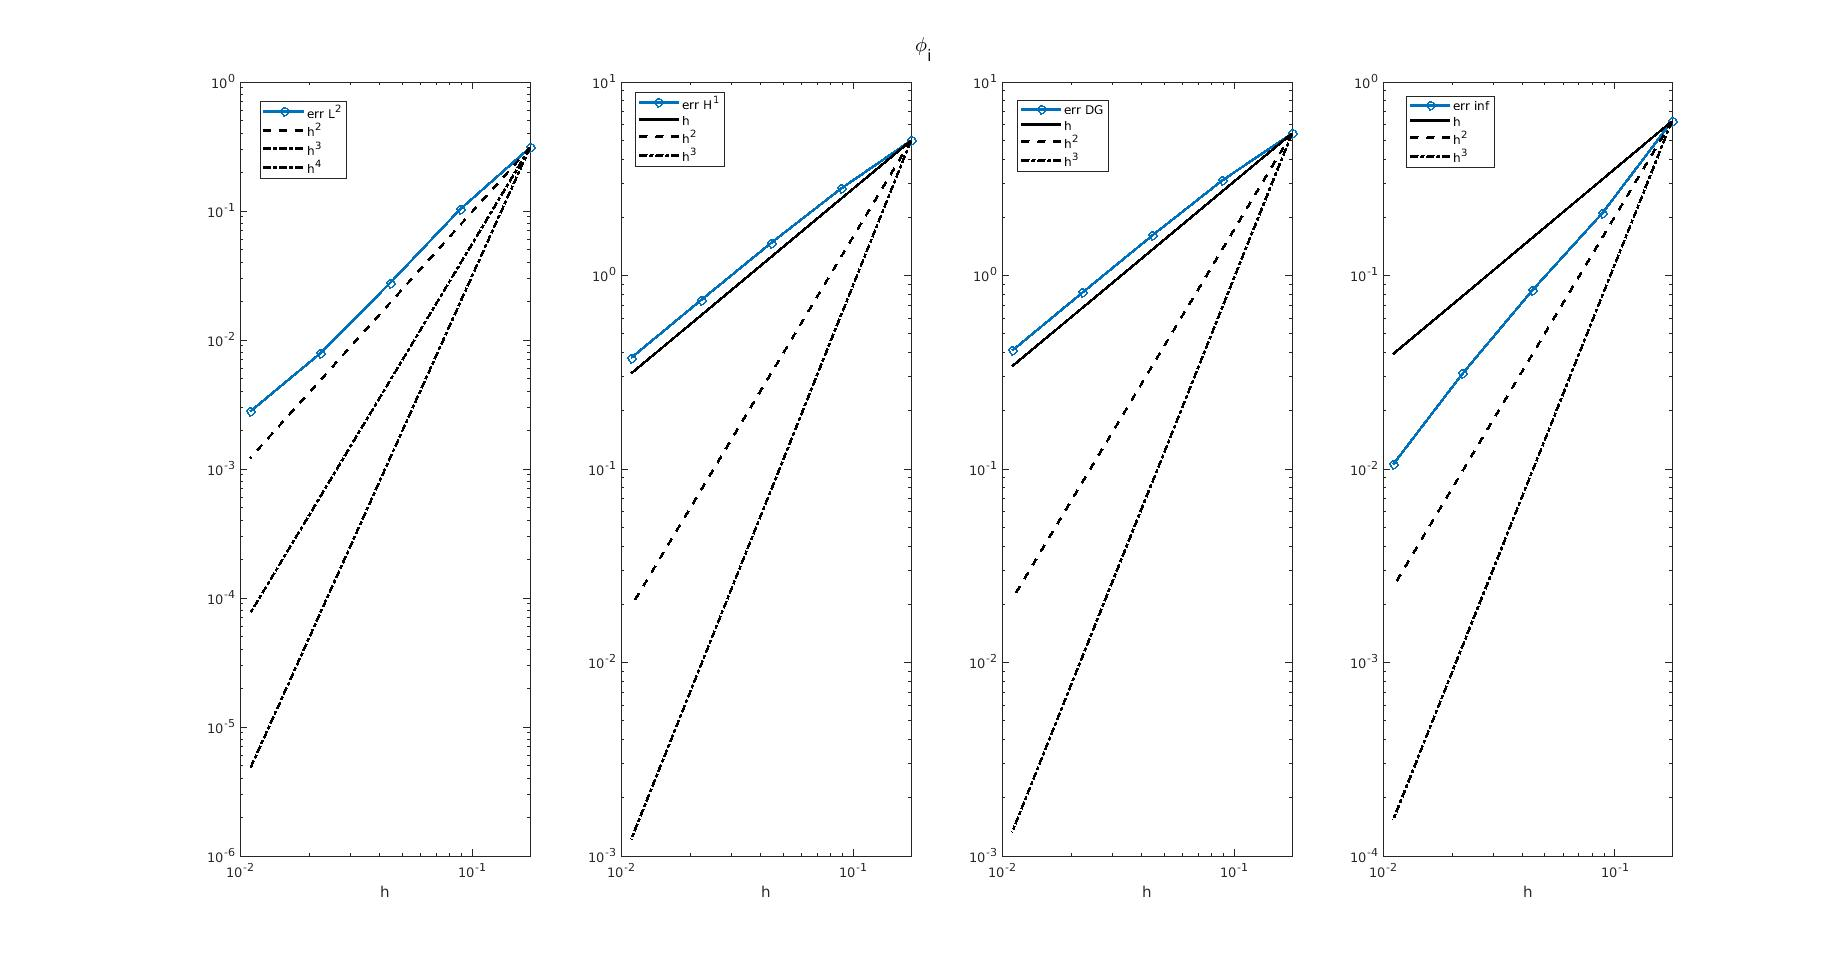
\includegraphics[width = 9cm]{./D1_Phii_1.jpg}
\caption*{$\phi_i$ with D1 imposing the function in a specific point}
\label{Phii_1}
\end{subfigure}
\begin{subfigure}{0.5\textwidth}
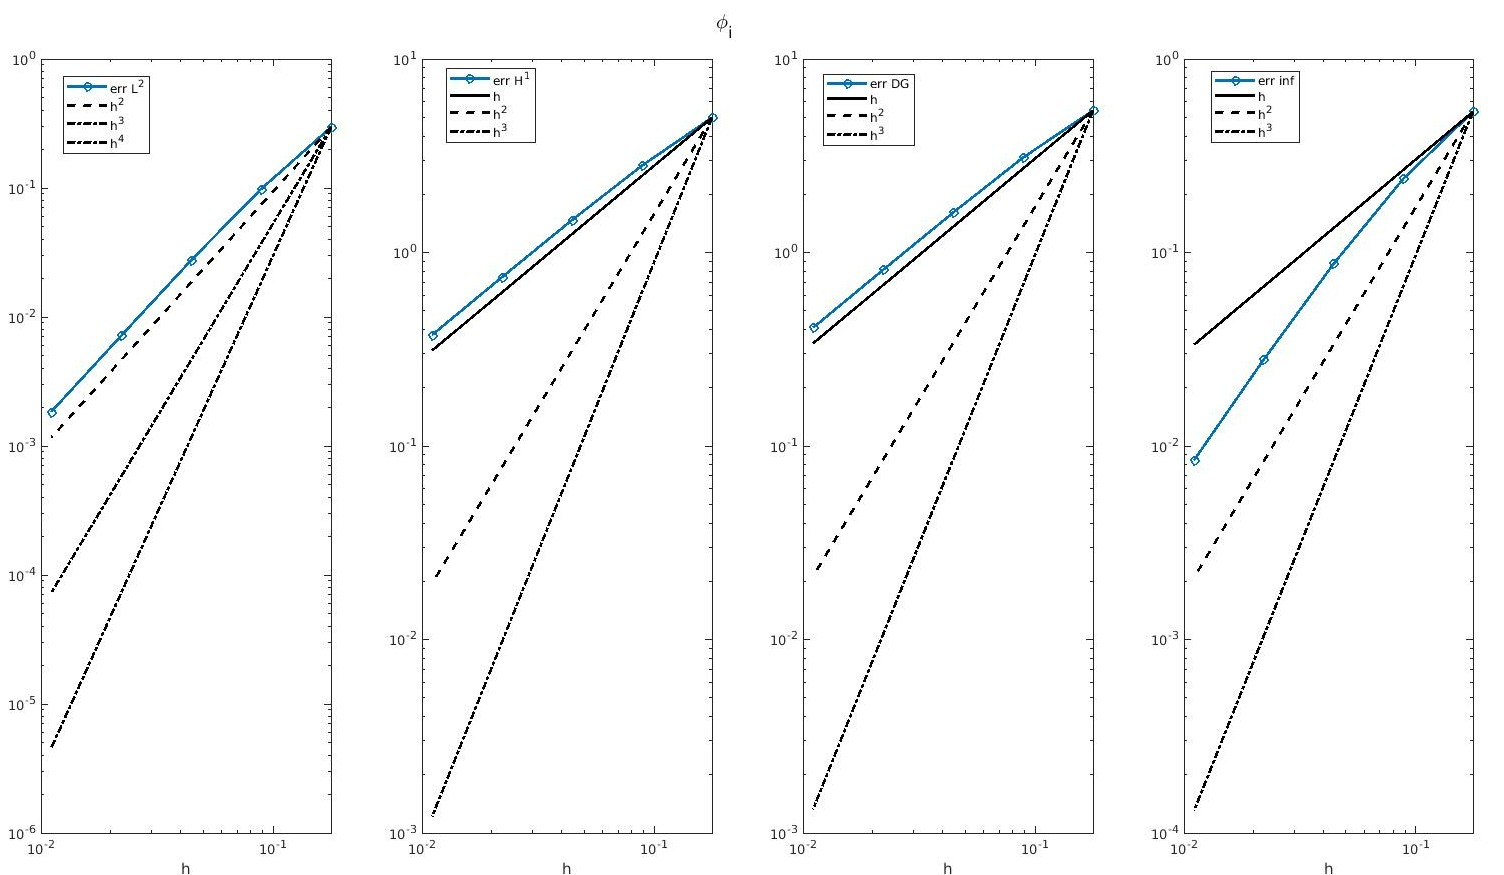
\includegraphics[width =9cm]{./D1_Phii_2.jpg}
\caption*{$\phi_i$ with D1 imposing the zero mean}
\label{Phii_2}
\end{subfigure}
\begin{subfigure}{0.5\textwidth}
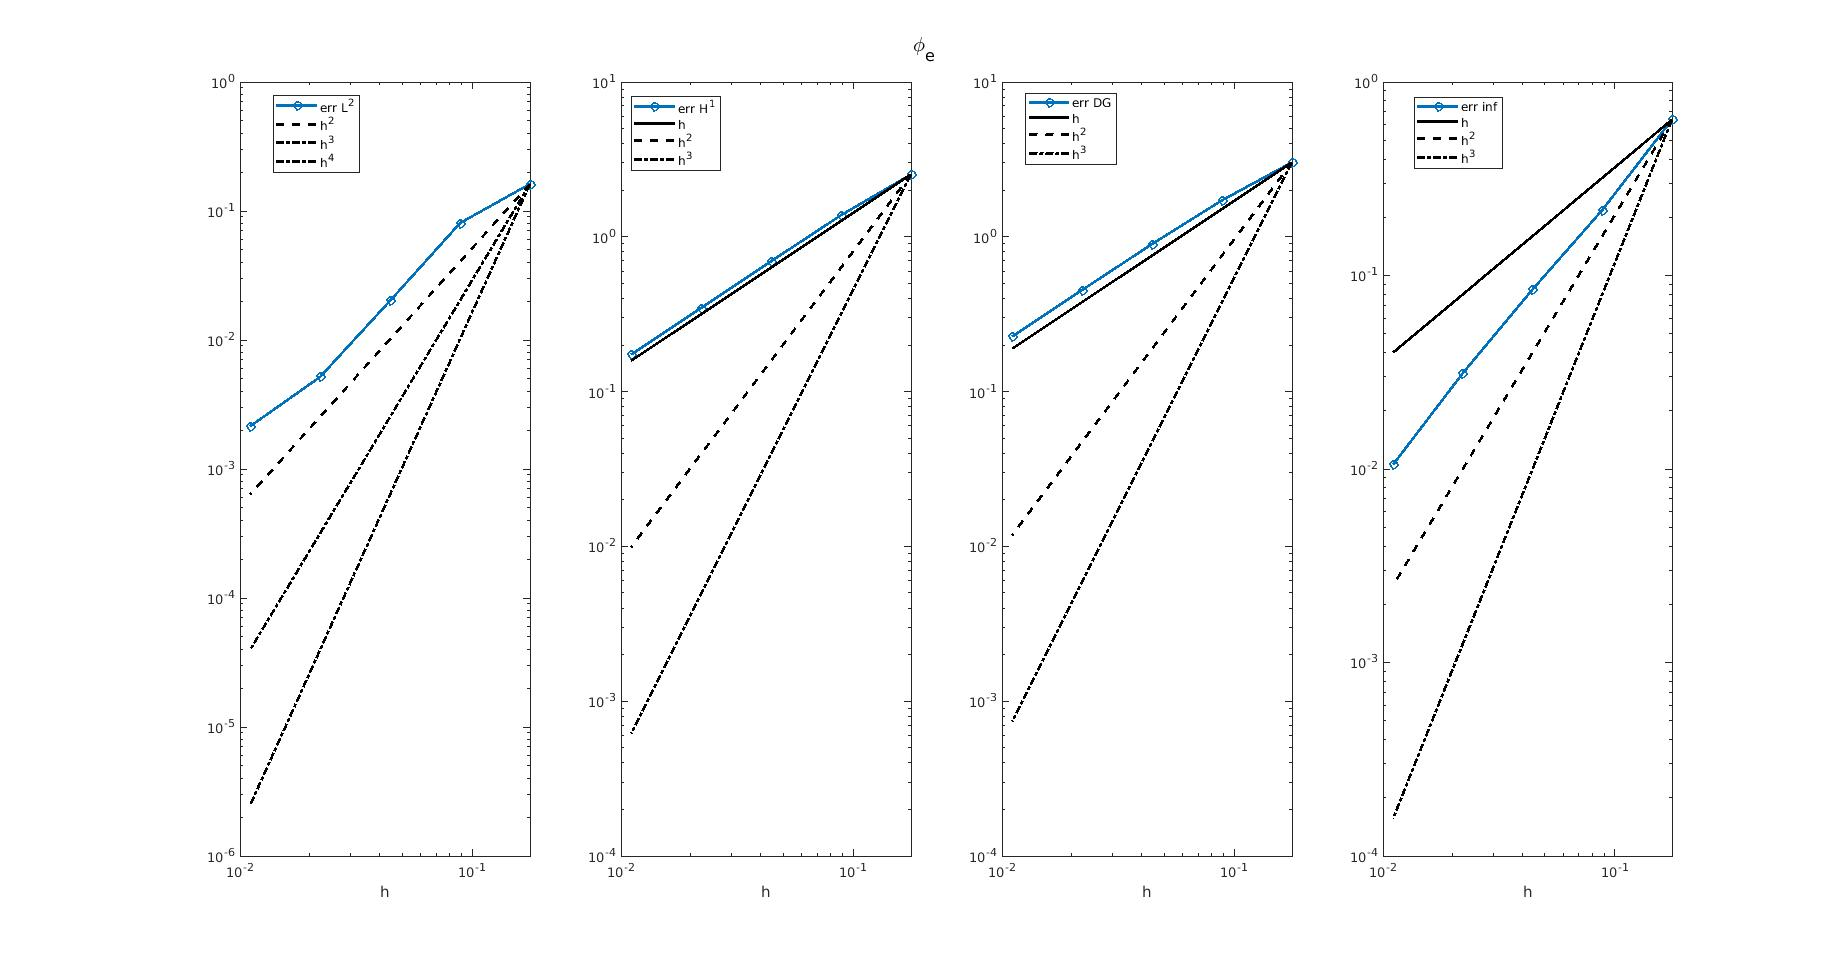
\includegraphics[width = 9cm]{./D1_Phie_1.jpg}
\caption*{$\phi_e$ with D1 imposing the function in a specific point}
\label{Phie_1}
\end{subfigure}
\begin{subfigure}{0.5\textwidth}
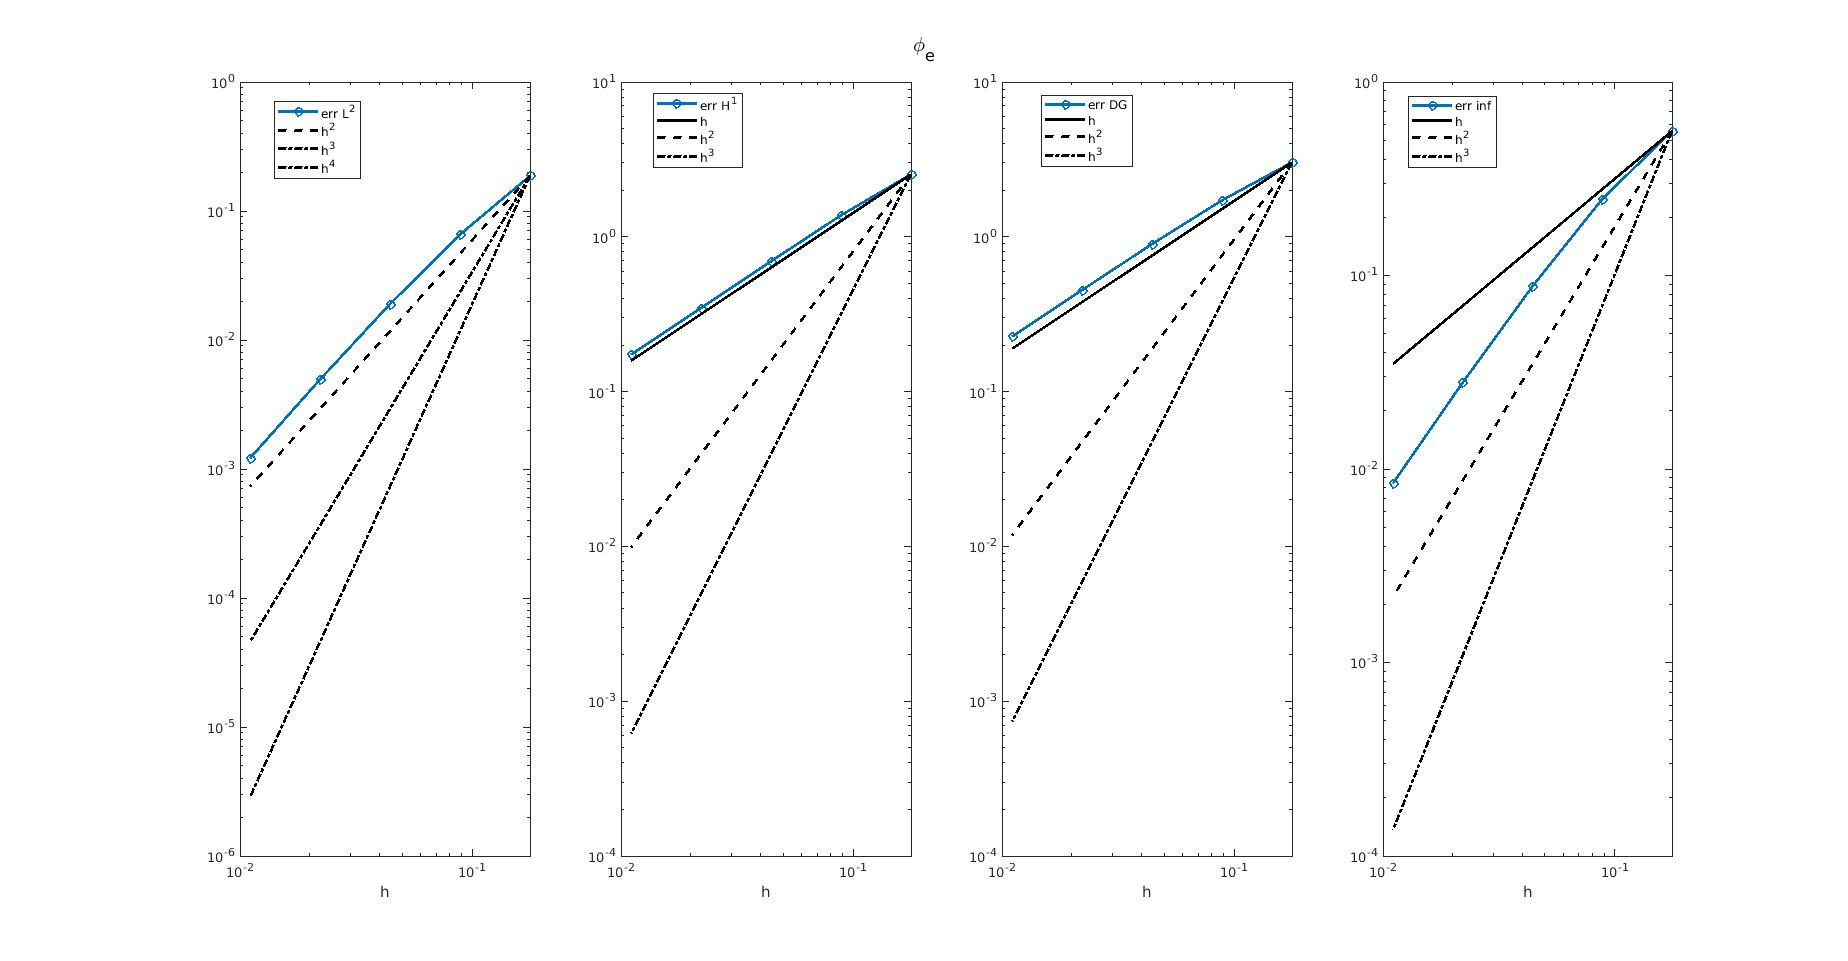
\includegraphics[width =9cm]{./D1_Phie_2.jpg}
\caption*{$\phi_e$ with D1 imposing the zero mean}
\label{Phie_2}
\end{subfigure}
\begin{subfigure}{0.5\textwidth}
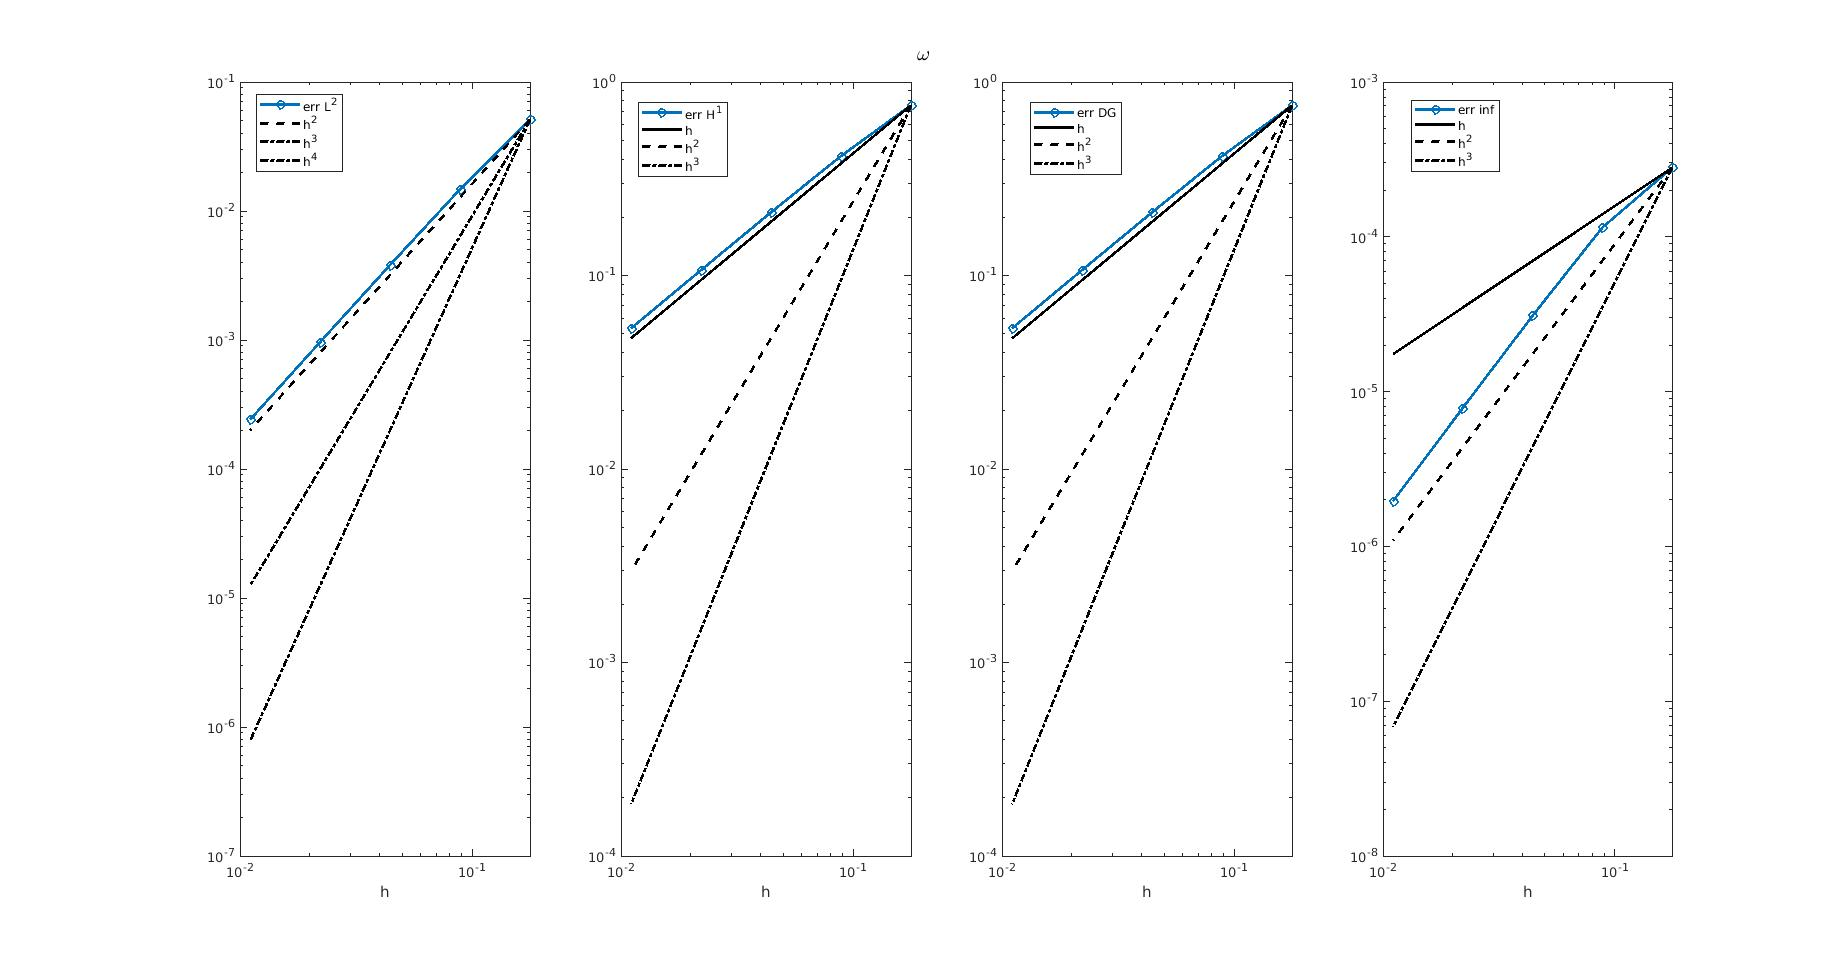
\includegraphics[width = 9cm]{./D1_w_1.jpg}
\caption*{$w$ with D1 imposing the function in a specific point}
\label{w_1}
\end{subfigure}
\begin{subfigure}{0.5\textwidth}
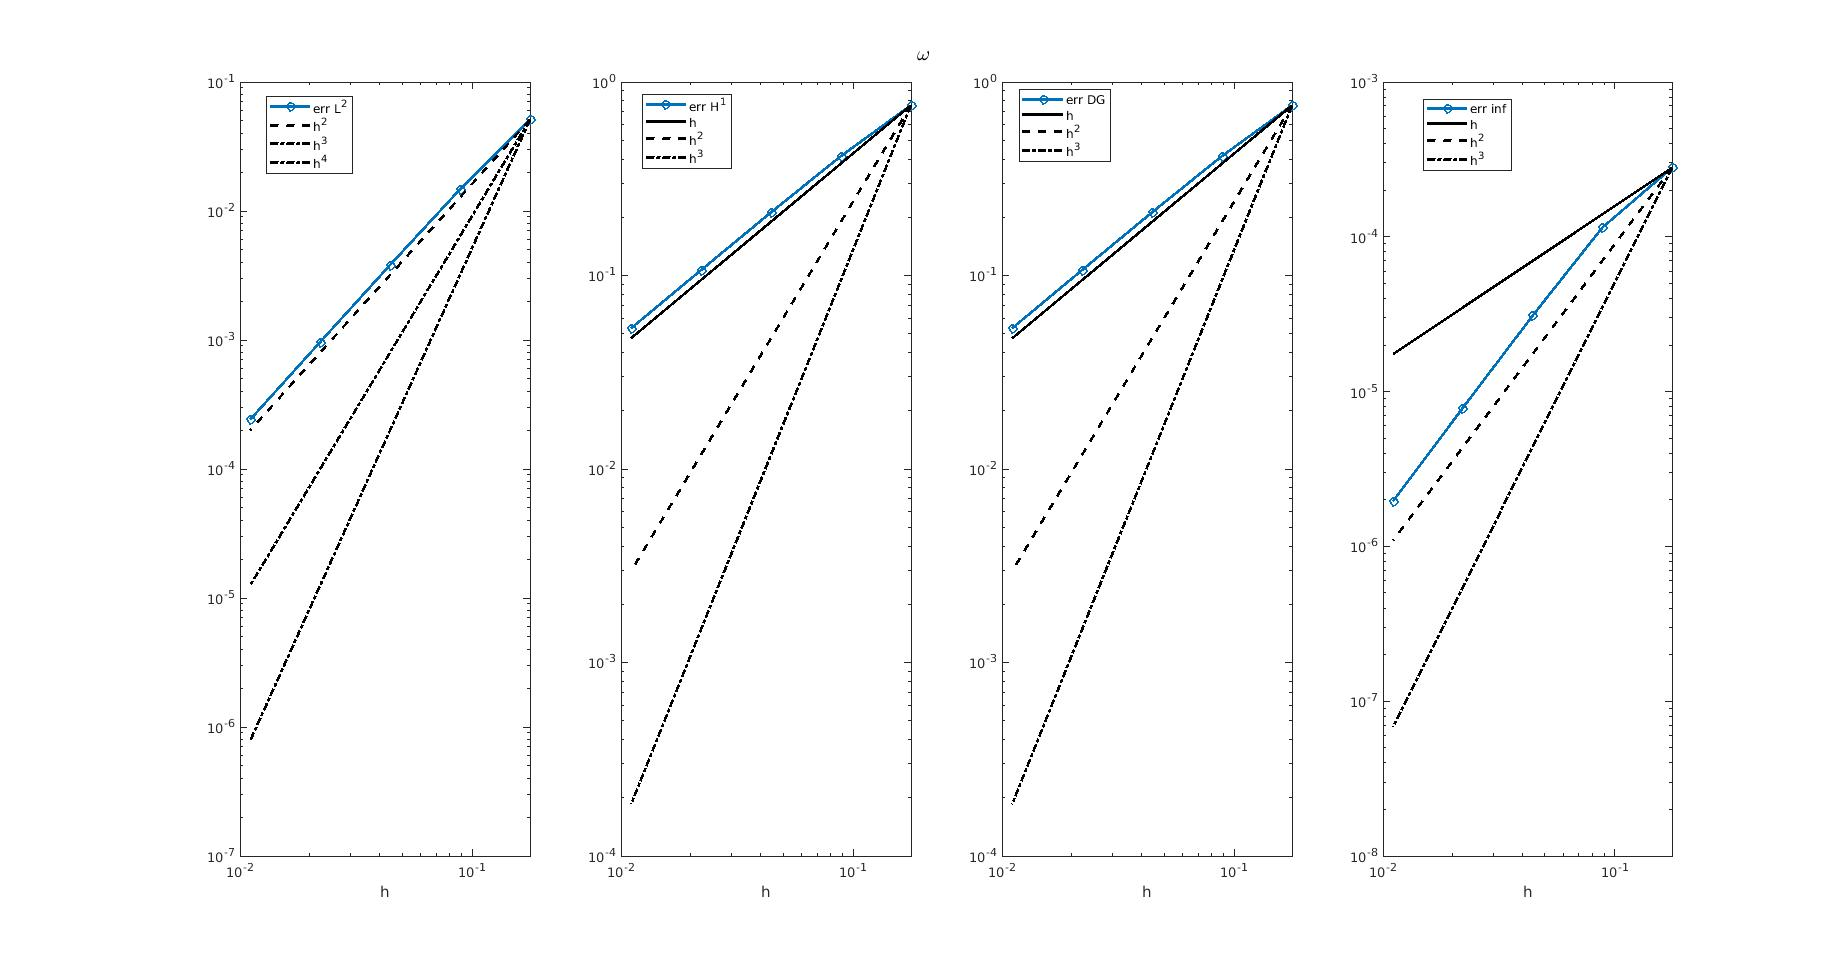
\includegraphics[width =9cm]{./D1_w_2.jpg}
\caption*{$w$ with D1 imposing the zero mean}
\label{w_2}
\end{subfigure}
\end{figure}
\restoregeometry
\newpage
\section{Realistic simulations} \label{real_sim}
Our final goal is to exploit strategies and tools presented in the previous sections to run simulations that can get closer to the cardiac electrophysiology phenomena. It is noteworthy to warn that no exact solutions are known for these kinds of problems and what we care about is only visual. Moreover, we warn that there are some limitations to the complete resemblance to the realistic phenomena, for instance the domain shape. Our general choices for all the test-cases are the following:

\begin{center}
	\captionof{table}{Parameters for pseudo-realistic simulations}
	\begin{tabular}{|c|c|} 
		\hline 
		\rule[-4mm]{0mm}{1cm}
		Domain & $\begin{bmatrix} -0.025 & 0.035 \\ -0.025 & 0.035\end{bmatrix}$ \\
		\hline
		\rule[-4mm]{0mm}{1cm}
		Temporal scheme & Semi-implicit \\
		\hline
		\rule[-4mm]{0mm}{1cm}
		Polynomials space & D1 \\
		\hline
		\rule[-4mm]{0mm}{1cm}
		$dt$ & 0.0001 \\
		\hline
		\rule[-4mm]{0mm}{1cm}
		$nREF$ & 5 \\ 
		\hline
		\rule[-4mm]{0mm}{1cm}
		Initial condition for $V_m$ & 0 \\
		\hline
		\rule[-4mm]{0mm}{1cm}
		Initial condition for $w$ & 0 \\
		\hline
		\rule[-4mm]{0mm}{1cm}
		$I_i^{ext}$ & $I \cdot 10^3 \, \chi_{[0.001,0.002]}(t) \, \chi_{[0.0045,0.0055]}(x) \, \chi_{[0.0045,0.0055]}(y)$ \\
		\hline
		\rule[-4mm]{0mm}{1cm}
		$I_e^{ext}$ & $I \cdot 10^3 \, \chi_{[0.001,0.002]}(t) \, \chi_{[0.0045,0.0055]}(x) \, \chi_{[0.0045,0.0055]}(y)$ \\
		\hline
		\rule[-4mm]{0mm}{1cm}
		$b_i$ & 0 \\
		\hline
		\rule[-4mm]{0mm}{1cm}
		$b_e$ & 0 \\
		\hline 
		\rule[-4mm]{0mm}{1cm}
		$\chi_m$ & $10^5$ \\
		\hline 
		\rule[-4mm]{0mm}{1cm}
		$C_m$ & $10^{-2}$ \\
		\hline
		\rule[-4mm]{0mm}{1cm}
		$\Sigma_i$ & $\begin{bmatrix} 0.34 & 0 \\ 0 & 0.06\end{bmatrix}$ \\
		\hline
		\rule[-4mm]{0mm}{1cm}
		$\Sigma_e$ & $\begin{bmatrix} 0.62 & 0 \\ 0 & 0.24 \end{bmatrix}$ \\
		\hline 
	\end{tabular}
\end{center}
 \vspace{4mm}
\noindent Where $I$ is a positive value to be chosen depending on the context. We remind that the mean value imposition is always chosen for realistic simulations. Moreover, we observe that the main differences with the previous parameters are the square domain that is no more unitary and the anisotropy of the diffusion tensors. The latter choice is motivated from the real utility of the \emph{Bidomain Model} if compared to the \emph{Monodomain Model}, where the two tensors are assumed to be equal or proportional. Parameters values are taken as usual from literature, especially from \cite{acta}. \\

\noindent Physically, this setting represents a square section of the surface of the heart that is electrically isolated (homogeneous boundary conditions) and an external current that is applied in a central region for a limited interval of time. \\
To conclude, observe that the compatibility condition for the existence of the solution is satisfied since both boundary conditions and external currents are the same in the intracellular and extracellular regions. \\

\noindent For what concerns \emph{FitzHugh-Nagumo} parameters, there are no general values as for the previous ones. To generalize this aspect, we defined two different test-cases with two different sets of parameters, namely:

\begin{center}
	\captionof{table}{FitzHugh-Nagumo Parameters for pseudo-realistic simulations}
	\begin{tabular}{|c|c|c|} 
		\hline 
		 & Test-case 1 & Test-case 2 \\
		\hline \hline
		$k$ & $19.5 $ & 1 \\
		\hline
		$\epsilon$ & $1.2$ & $0.2232$ \\ 
		\hline
		$\gamma$ & $0.1$ & $4.0322$ \\
		\hline
		$a$ & $13\cdot 10^{-3}$ & 0.004 \\
		\hline
	\end{tabular}
\end{center}

\vspace{4mm}
\noindent Basically, the first test-case comes from the values already adopted for Section (\ref{error_analysis}) and taken from past projects \cite{bagnara},\cite{andreotti}, \cite{marta}. On the other hand, second test-case comes from \cite{mauricio}.

\subsection{First test-case}
For both the test-cases, we aim to show two different situations depending on the external current intensity: firstly, for too weak currents, the electrical activation should miss and this implies that the potentials are not capable to hold up. Secondly, if the intensity is over a certain threshold, we should see the electrical activation and the resulting diffusion. Several simulations have proved that:
\begin{itemize}
	\item $I = 500 \cdot 10^3 $ is a suitable value for the \emph{underflow} case.
	\item $I = 700 \cdot 10^3 $ is a suitable value for the \emph{overflow} case.
\end{itemize}

\noindent Visual results are the following:
\newpage
\newgeometry{a4paper,top=1cm,bottom=2cm,left=1cm,right=1cm} 
\begin{figure}[h] \captionsetup{size = large} \caption{Test-case 1, activation missed ($I=500 \cdot 10^3$)}
	\centering
	\begin{subfigure}{0.4\textwidth}
		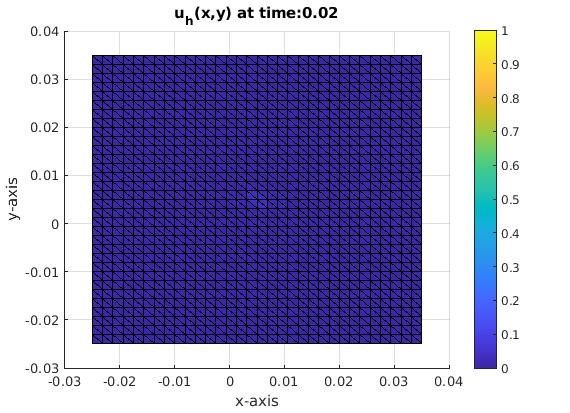
\includegraphics[width = 8cm]{./tc1-1/002.jpg}
	\end{subfigure}
	\begin{subfigure}{0.4\textwidth}
		\includegraphics[width =8cm]{./tc1-1/004.jpg}
	\end{subfigure}
	\begin{subfigure}{0.4\textwidth}
		\includegraphics[width = 8cm]{./tc1-1/006.jpg}
	\end{subfigure}
	\begin{subfigure}{0.4\textwidth}
		\includegraphics[width =8cm]{./tc1-1/008.jpg}
	\end{subfigure}
	\begin{subfigure}{0.4\textwidth}
		\includegraphics[width = 8cm]{./tc1-1/010.jpg}
	\end{subfigure}
	\begin{subfigure}{0.4\textwidth}
		\includegraphics[width =8cm]{./tc1-1/012.jpg}
	\end{subfigure}
	\begin{subfigure}{0.4\textwidth}
		\includegraphics[width = 8cm]{./tc1-1/014.jpg}
	\end{subfigure}
	\begin{subfigure}{0.4\textwidth}
		\includegraphics[width =8cm]{./tc1-1/016.jpg}
	\end{subfigure}
\end{figure}
\restoregeometry
\newpage
\newgeometry{a4paper,top=1cm,bottom=2cm,left=1cm,right=1cm} 
\begin{figure}[h] \captionsetup{size = large} \caption{Test-case 1, activation achieved ($I = 700 \cdot 10^3$)}
	\centering
	\begin{subfigure}{0.4\textwidth}
		\includegraphics[width = 8cm]{./tc1-2/002.jpg}
	\end{subfigure}
	\begin{subfigure}{0.4\textwidth}
		\includegraphics[width =8cm]{./tc1-2/004.jpg}
	\end{subfigure}
	\begin{subfigure}{0.4\textwidth}
		\includegraphics[width = 8cm]{./tc1-2/006.jpg}
	\end{subfigure}
	\begin{subfigure}{0.4\textwidth}
		\includegraphics[width =8cm]{./tc1-2/008.jpg}
	\end{subfigure}
	\begin{subfigure}{0.4\textwidth}
		\includegraphics[width = 8cm]{./tc1-2/010.jpg}
	\end{subfigure}
	\begin{subfigure}{0.4\textwidth}
		\includegraphics[width =8cm]{./tc1-2/012.jpg}
	\end{subfigure}
	\begin{subfigure}{0.4\textwidth}
		\includegraphics[width = 8cm]{./tc1-2/014.jpg}
	\end{subfigure}
	\begin{subfigure}{0.4\textwidth}
		\includegraphics[width =8cm]{./tc1-2/016.jpg}
	\end{subfigure}
\end{figure}
\restoregeometry
\newpage
\subsection{Second test-case}
For these modified parameters, the threshold for the activation is different as we can state that:
\begin{itemize}
	\item $I = 15000 \cdot 10^3 $ is a suitable value for the \emph{underflow} case.
	\item $I = 20000 \cdot 10^3 $ is a suitable value for the \emph{overflow} case.
\end{itemize}

\noindent Results related to this test-case are visible in Fig. (\ref{tc2-1}) and Fig. (\ref{tc2-2}).

\subsection{Comments on the results}
As expected, we can distinguish two different phenomena in both the test-cases:
\begin{itemize}
	\item In \emph{underflow} simulations, propagation is visible and wave height (that is always below 1) decreases at every time-step. Then, the overall phenomena seems to be only diffusive.
	\item On the contrary, in \emph{overflow} simulations, propagation is visible and the wave height keeps constant with value $\approx 1$.  
\end{itemize}

\noindent On the other hand, the main differences due to the choice of \emph{FitzHugh-Nagumo} parameters turn to be:
\begin{itemize}
	\item The threshold intensity (in test-case 2 this value is ten times the first).
	\item The speed of propagation (test-case 2 needs a lot more time to activate all the domain, 0.6 seconds are still not sufficient).
	\item The direction of propagation (shape in test-case 2 is more symmetric).
\end{itemize}
 
\noindent Most of these features were expected and successfully reflect the physical phenomenon. Indeed, a certain current intensity is needed to fully activate the myocyties. Otherwise, cells go soon back to their rest potential. Moreover, the stretched shape of the activated region is consistent with the anisotropy of the diffusion tensor and it physically shows the difference of conductivity between the tangential and normal direction of the fibers.\\

\noindent On the other hand, if we look at the potential cycle shown in Fig. (\ref{potential_cycle}), we notice some unexpected mismatches. First of all, the rest and activation values should be $-0.09V$ and $0.02V$ and not $0V$ and $1V$. However, it is probably due to the extremely simplicity of the \emph{FitzHugh-Nagumo} model that we adopted. Just from the analytical formulation is clear that $V_m=0$ is an equilibrium value and not $V_m=-0.09$, then a refinement to the model is needed to get these more realistic values. \\
The second and more sophisticated incongruence is the missed repolarization after the activation. In other words, the potential keeps the same value and it does not decrease back to 0 even after several time-steps. We think it is in part due to (again) the simplicity of the \emph{FitzHugh-Nagumo} model, fact that is moreover warned in \cite{colli_franzone_parallel}. Here, it is indeed stated that \emph{FitzHugh-Nagumo} model is not able to truly approximate the physical phenomenon, in particular for the \emph{plateau} and \emph{repolarization} phases.

\newpage
\newgeometry{a4paper,top=1cm,bottom=2cm,left=1cm,right=1cm} 
\begin{figure}[h] \captionsetup{size = large} \caption{Test-case 2, activation missed ($I = 15000 \cdot 10^3$)} \label{tc2-1}
	\centering
	\begin{subfigure}{0.4\textwidth}
		\includegraphics[width = 8cm]{./tc2-1/004.jpg}
	\end{subfigure}
	\begin{subfigure}{0.4\textwidth}
		\includegraphics[width =8cm]{./tc2-1/012.jpg}
	\end{subfigure}
	\begin{subfigure}{0.4\textwidth}
		\includegraphics[width = 8cm]{./tc2-1/020.jpg}
	\end{subfigure}
	\begin{subfigure}{0.4\textwidth}
		\includegraphics[width =8cm]{./tc2-1/028.jpg}
	\end{subfigure}
	\begin{subfigure}{0.4\textwidth}
		\includegraphics[width = 8cm]{./tc2-1/036.jpg}
	\end{subfigure}
	\begin{subfigure}{0.4\textwidth}
		\includegraphics[width =8cm]{./tc2-1/044.jpg}
	\end{subfigure}
	\begin{subfigure}{0.4\textwidth}
		\includegraphics[width = 8cm]{./tc2-1/052.jpg}
	\end{subfigure}
	\begin{subfigure}{0.4\textwidth}
		\includegraphics[width =8cm]{./tc2-1/060.jpg}
	\end{subfigure}
\end{figure}
\restoregeometry
\newpage
\newgeometry{a4paper,top=1cm,bottom=2cm,left=1cm,right=1cm} 
\begin{figure}[h] \captionsetup{size = large} \caption{Test-case 2, activation achieved ($I = 20000 \cdot 10^3$)} \label{tc2-2}
	\centering
	\begin{subfigure}{0.4\textwidth}
		\includegraphics[width = 8cm]{./tc2-2/004.jpg}
	\end{subfigure}
	\begin{subfigure}{0.4\textwidth}
		\includegraphics[width =8cm]{./tc2-2/012.jpg}
	\end{subfigure}
	\begin{subfigure}{0.4\textwidth}
		\includegraphics[width = 8cm]{./tc2-2/020.jpg}
	\end{subfigure}
	\begin{subfigure}{0.4\textwidth}
		\includegraphics[width =8cm]{./tc2-2/028.jpg}
	\end{subfigure}
	\begin{subfigure}{0.4\textwidth}
		\includegraphics[width = 8cm]{./tc2-2/036.jpg}
	\end{subfigure}
	\begin{subfigure}{0.4\textwidth}
		\includegraphics[width =8cm]{./tc2-2/044.jpg}
	\end{subfigure}
	\begin{subfigure}{0.4\textwidth}
		\includegraphics[width = 8cm]{./tc2-2/052.jpg}
	\end{subfigure}
	\begin{subfigure}{0.4\textwidth}
		\includegraphics[width =8cm]{./tc2-2/060.jpg}
	\end{subfigure}
\end{figure}
\restoregeometry
\newpage
\section{Conclusion}
After some introductions and motivations, we have validated our numerical study through a basic error analysis and a couple of simulations aimed to re-create what happens in the human heart.
\noindent From the former we obtained excellent validations: every result was consistent with the theory and even what was initially unexpected has later been justified with other causes independent from our study.\\
\noindent From the latter, we achieved very good outcomes too: our simulations turned to be consistent with the physical phenomenon except for the missed repolarization. We doubt that it is due to the numerical schemes because of the excellent results in the error analysis. We instead suppose it is due to the extreme simplicity of the ionic model taken into consideration. Some inconsistencies may also be caused by a too wide mesh, something that we could not avoid to get results in a reasonable time. Further researches could then consider a mesh-adaptivity study (even if it requires very powerful computers) and/or the adoption of other ionic models.
\noindent We hope that this last point could be a springboard for future projects aiming at improving and generalize our results. 
\section{Appendix: numerical codes}
\subsection{\texttt{dubiner\_to\_fem.m}}\label{dub_to_fem}
\begin{lstlisting}[language=Matlab,basicstyle=\small, numbers=left, numberstyle=\tiny,  name = dubiner_to_fem.m, frame=single]
function [u0] = dubiner_to_fem (uh, femregion, Data)  
	
...
...
...
	
u0 = zeros(femregion.ndof,1);
	
% loop over all the elements
for ie = 1:femregion.ne
	
   % to get the global indexes for the nodes of ie 
   nln = femregion.nln;
   index = (ie-1)*nln*ones(nln,1) + [1:nln]';
	
   for i = 1 : nln
      for j = 1 : nln
         u0(index(i)) = u0(index(i)) +  uh(index(j))*phi(1,i,j);
      end
   end
end
\end{lstlisting} 

\subsection{\texttt{fem\_to\_dubiner.m}}\label{fem_to_dub}
\begin{lstlisting}[language=Matlab,basicstyle=\small, numbers=left, numberstyle=\tiny,  name = fem_to_dubiner.m, frame=single]
function [u0] = fem_to_dubiner (uh, femregion, Data)
	
...
...
...
	
u0 = zeros(femregion.ndof,1);
	
% loop over all the elements
for ie = 1:femregion.ne
	
   % to get the global indexes for the nodes of ie 
   nln = femregion.nln;
   index = (ie-1)*nln*ones(nln,1) + [1:nln]';
   % loop over local degrees of freedom
   for i = 1 : nln
      % loop over 2D quadrature points
      for k = 1:length(w_2D) 
         uh_eval_k = 0;
         % loop to evaluate uh in a quadrature point
         for j = 1 : nln
            uh_eval_k = uh_eval_k + uh(index(j))*phi_fem(1,k,j);
         end
         u0(index(i))=u0(index(i))+uh_eval_k*phi_dub(1,k,i).*w_2D(k);
      end
   end    
end
\end{lstlisting}
\subsection{\texttt{main2D.m} (semi-implicit method)}\label{SI}
\begin{lstlisting}[language=Matlab,basicstyle=\small, numbers=left, numberstyle=\tiny,  name = main2D.m (semi-implicit), frame=single]
MASS = [M -M; -M M];
ZERO = sparse(length(M), length(M));
MASS_W = [M ZERO; ZERO -M];
STIFFNESS = [Ai ZERO; ZERO  Ae];

for t=dt:dt:T

   w1 = 1/(1+epsilon*gamma*dt)*(w0+epsilon*dt*Vm0);
   w1=cat(1,w1, w1);
   Vm0 = cat(1,Vm0,Vm0);

   fi = assemble_rhs_i(femregion,neighbour,Data,t);
   fe = assemble_rhs_e(femregion,neighbour,Data,t);
   f1 = cat(1, fi, fe);

   [C] = assemble_nonlinear(femregion,Data,Vm0);
   NONLIN = [C -C; -C C];

   r = f1 + ChiM*Cm/dt * MASS_W * Vm0 - ChiM * MASS_W *w1;

   B=ChiM*Cm/dt * MASS + (STIFFNESS + NONLIN);

   u1 = B \ r;

   f0 = f1;
   Vm0 = u1(1:ll)-u1(ll+1:end);
   u0 = u1;
   w0 = w1(1:ll);
end
\end{lstlisting}

\subsection{\texttt{main2D.m} (Godunov operator-splitting method)}\label{GO}
\begin{lstlisting}[language=Matlab,basicstyle=\small, numbers=left, numberstyle=\tiny,  name = main2D.m (Godunov operator-splitting), frame=single]
ZERO = sparse(ll,ll);
MASS = (ChiM*Cm/dt)*[M, -M; M -M];
MASSW = ChiM*[M, ZERO; ZERO, M];

for t=dt:dt:T

   fi = assemble_rhs_i(femregion,neighbour,Data,t);
   fe = assemble_rhs_e(femregion,neighbour,Data,t);
   f1 = cat(1, fi, -fe);

   [C] = assemble_nonlinear(femregion,Data,Vm0);

   w1 = (1 -epsilon*gamma*dt)*w0 + epsilon*dt*Vm0;
   B = MASS + [Ai, ZERO; ZERO, -Ae];
   r = -MASSW*[w0;w0] + ((Cm/dt)*MASSW - [C, ZERO; ZERO, C])
   *[Vm0;Vm0] + f1;

   Vm0 = u1(1:ll) - u1(ll+1:end);
   u0 = u1;
   w0 = w1;
end
\end{lstlisting}

\subsection{\texttt{main2D.m} (quasi-implicit operator-splitting method)}\label{OS}
\begin{lstlisting}[language=Matlab,basicstyle=\small, numbers=left, numberstyle=\tiny,  name = main2D.m (quasi-implicit operator-splitting), frame=single]
ZERO = sparse(ll,ll);
        
for t=dt:dt:T
        
   [C] = assemble_nonlinear(femregion,Data,Vm0);
   Q  = (ChiM*Cm/dt)*M + C - (epsilon*ChiM*dt)/(1+epsilon*gamma*dt)*M;
   R  = (ChiM*Cm/dt)*M*Vm0 - (ChiM)/(1+epsilon*gamma*dt)*M*w0;
    
   fi = assemble_rhs_i(femregion,neighbour,Data,t);
   fe = assemble_rhs_e(femregion,neighbour,Data,t);
   f1 = cat(1, fi, -fe);
    
   B = [Q, -Q; Q, -Q] + [Ai, ZERO; ZERO, -Ae];
   r = [R;R] + f1;
        
   u1 = B \ r; 
        
   Vm1 = u1(1:ll)-u1(ll+1:end);

   w1 = (w0 + epsilon*dt*Vm1)/(1+epsilon*gamma*dt);
    
   f0 = f1;
   Vm0 = u1(1:ll) - u1(ll+1:end);
   u0 = u1;
   w0 = w1;
end
\end{lstlisting}
\subsection{\texttt{assign\_phi\_i.m}}\label{assign}
\begin{lstlisting}[language=Matlab,basicstyle=\small, numbers=left, numberstyle=\tiny,  name = assign_phi_i.m, frame=single]
function [A, b] = assign_phi_i (A, b, t, Data, femregion)

...
...
...

if (Data.fem(1)=='P')

   x = femregion.dof(1,1); % x-coordinate of the first dof point
   y = femregion.dof(1,2); % y-coordinate of the first dof point
   exact_coeff = eval(Data.exact_sol_i); % evaluation of exact sol


elseif (Data.fem(1)=='D')
   x0=femregion.dof(3,1); % bottom-left corner of the first element
   y0=femregion.dof(3,2);
   h=femregion.dof(1,1)-femregion.dof(3,1); % length of the element

   exact_coeff = 0;
   index = 1;
   
   ...
   ...
   ...

   % the first coeff is the L2 scalar product of uh with the first
   % basis function. To the get the right coeff, we compute the scalar 
   % product between the exact solution and the first basis function
   
   for k = 1:length(w_2D) % loop over 2D quadrature points
      %physical coords of the integration point
      x = x0 + h*node_2D(k,1);  
      y = y0 + h*node_2D(k,2);
      evalsol = eval(Data.exact_sol_i);
      exact_coeff = exact_coeff + evalsol*phi_dub(1,k,index).*w_2D(k);
   end

end


% we change the system coefficients to impose u(1)=exact_coeff
Nh = length(b);
b = b - A(:,1)*exact_coeff;
b(1) = exact_coeff;  
A(:,1) = zeros(Nh,1);
A(1,:) = zeros(1,Nh);
A(1,1) = 1;
\end{lstlisting}
\subsection{\texttt{assign\_null\_average.m}}\label{mean}
\begin{lstlisting}[language=Matlab,basicstyle=\small, numbers=left, numberstyle=\tiny,  name = assign_null_average.m, frame=single]
function [A, b] = assign_null_average (A, b, Data, femregion)

Nh = length(b)/2;

if (Data.fem(1)=='P')

   ...
   ...
   ...

   for k = 1:length(w_2D)
      coeff = coeff + phi_fem(1,k,1).*w_2D(k);
   end

   for i = 1:Nh
      A(i,2*Nh+1)=coeff;
      A(2*Nh+1,i)=coeff;
   end


elseif (Data.fem(1)=='D')

   ...
   ...
   ...

   for p = 1:femregion.nln
      p_int = 0;
      for k = 1:length(w_2D)
         p_int = p_int + phi_dub(1,k,p).*w_2D(k);
      end
      coeff(p)=p_int;
   end

   for i = 1:femregion.nln:Nh
      A(2*Nh+1,i:i+femregion.nln-1)=coeff';
      A(i:i+femregion.nln-1,2*Nh+1)=coeff;
   end

end

b = [b;0];

\end{lstlisting}
    \newpage ~\newpage
    \printbibliography

\end{document}

    
	
    
    
    
    
    
    
    
    
    
    
    
    \newpage
    \printbibliography

\end{document}
